\documentclass[11pt, paper=a4]{scrartcl}

% CONFIG
\newcommand{\exptitle}{Optical pumping}       % long name of experiment 
\newcommand{\exptitleshort}{Optical pumping} % short name of experiment
\newcommand{\expdate}{11.04.2016}           % date of experiment
\newcommand{\exptutor}{Dominik Schomas}

% PACKAGES + MODIFICATIONS
%\usepackage[ngerman]{babel} %standard language stuff
\usepackage[T1]{fontenc}
\usepackage[utf8]{inputenc}
\usepackage{textgreek}

\usepackage{soul} %better underline
\setul{2pt}{.4pt} %set underline 2 pts below text and thickness to .4pt

\usepackage[fleqn]{amsmath}  % math
\usepackage{amssymb}

\usepackage{graphicx} %graphics
\usepackage{float} 

\usepackage[automark,headsepline]{scrlayer-scrpage} %headings
\pagestyle{scrheadings}
\ihead{\exptitleshort}
\ohead{\pagemark}
\cfoot{}

\usepackage{hyperref}
\hypersetup{
    unicode=true,          % non-Latin characters in Acrobat’s bookmarks
    pdftoolbar=true,       % show Acrobat’s toolbar?
    pdfmenubar=true,       % show Acrobat’s menu?
    pdffitwindow=false,    % window fit to page when opened
    pdfstartview={FitH},   % fits the width of the page to the window
    pdfnewwindow=true,     % links in new window
    colorlinks=true,       % false: boxed links; true: colored links
    linkcolor=blue,       % color of internal links (change box color with linkbordercolor)
    citecolor=green,       % color of links to bibliography
    filecolor=magenta,     % color of file links
    urlcolor=blue          % color of external links
}

\usepackage[labelfont=bf]{caption} % bold captions

\usepackage{chngcntr} % change behaviour of counters in different environments
\counterwithin{figure}{section}  % number figures per section
\numberwithin{equation}{section} % number equations per section
\numberwithin{table}{section}    % number tables per section

\usepackage{enumerate} % better way to config enumerates

\setcounter{tocdepth}{2} % table of contents depth

\setlength{\parindent}{0pt} % no indent on new paragraph

\usepackage{pdfpages} % include pdf files

\usepackage[nottoc,numbib]{tocbibind} % bibliography in TOC

% NEW COMMANDS
\newcommand{\refeq}[1]{\overset{\text{\eqref{#1}}}{=}}

% DOCUMENT SETTINGS

\title{\exptitle}
\subtitle{}
\author{}
\date{\expdate}

% DOCUMENT
\begin{document}

\hypersetup{pageanchor=false} %stop page numbering (hyperref) to prevent for double page numers
\newcommand{\HRule}{\rule{\linewidth}{0.5mm}}
\begin{titlepage}
\begin{center}
  \textsc{\Large Fortgeschrittenen Praktikum II }\\[0.5cm]
  \HRule \\[0.4cm]
  { \huge \bfseries \exptitle}\\
  \HRule \\[0.5cm]
  \large \expdate\\[0.5cm]  
  Benjamin Winkelmann \\
  Peter Spalthoff \\
  \vspace{10pt}
  \large 
  Tutor: \exptutor \\[3cm]
  \vfill
  \normalsize
\end{center}
\end{titlepage}
\thispagestyle{empty}



\pagenumbering{Roman}
\setcounter{page}{1}


\section{Abstract}
Optical pumping between Zeeman states of rubidium isotopes $^{87}$Rb and $^{85}$Rb that are split up by well controlled magnetic fields allows for the precise calculation of the earths magnetic field, hyperfine constants $A$ of the two isotopes as well as the relaxation time of the polarized states. The resulting hyperfine constants were calculated as
\begin{align}
	A_{^2S_{\nicefrac{1}{2}}}(^{87}Rb)&=\unit{(14.61\pm0.13)}{\micro\electronvolt}\\
	A_{^2S_{\nicefrac{1}{2}}}(^{85}Rb)&=\unit{(4.50\pm0.08)}{\micro\electronvolt}\\
	A_{^2P_{\nicefrac{1}{2}}}(^{87}Rb)&=\unit{(1.52\pm0.18)}{\micro\electronvolt}
\end{align}
The hyperfine constant $A_{^2P_{\nicefrac{1}{2}}}(^{85}Rb)$ could not be calculated since the relevant peaks could not be separated with the set-up.
The earths' magnetic field components were calculated to be
\begin{align}
	B_v&=\unit{(37.1\pm1.4)}{\micro T}\\
	B_h&=\unit{(2.36\pm 0.21)}{\micro T}
\end{align}
Of the two methods used to calculate the relaxation times, only the Dehmelt method produced a reasonable result for the relaxation time:
\begin{equation}
T_R=\unit{(4.8\pm1.5)}{ms}
\end{equation}
\tableofcontents

\newpage
\listoffigures
\thispagestyle{empty}


\listoftables

\thispagestyle{empty}



\newpage
\hypersetup{pageanchor=false} %stop page numbering (hyperref) to prevent for double page numers

\clearpage
\pagenumbering{arabic}
\setcounter{page}{1}

\section{Goal of the experiment}
In this experiment, the process of optical pumping will be used to precisely measure properties of Rubidium atoms such as the hyperfine constant $A$ via absorption measurements. In addition to that, relaxation times of the induced pumped states as well as external magnetic fields will also be measured by observing the effect of magnetic fields, applied through Helmholtz coils, high frequency radio waves and variations in the laser intensity.
\section{Physical principles}
\subsection{Hyperfine structure and Zeeman splitting}
This section is based on the detailed elaborations in \cite{staatsex}.\\
The fine structure levels of the atomic spectrum, which splits the basic levels into sub-levels due to spin-orbit interaction, can be shown to be split into even finer levels, whose energetic distances are roughly three orders of magnitude smaller than those of the fine structure. This is called the 'hyperfine structure' and is mainly caused by the interaction of the nuclear magnetic dipole and quadrupole moment and the magnetic field of the shell electrons. Its structure for the two Rubidium isotopes that are used in this experiment can be seen in figure \ref{fig:hyperfinestructure}.\\

As the nucleus is charged and, expressed as the nuclear spin $\vec{I}$, has angular momentum, it also has a magnetic moment, which is $\vec{\mu}_I=\frac{g_I\mu_K}{\hbar}\vec{I}$, where $g_I$ is the g-factor of the nucleus and $\mu_K$ is the nuclear magneton. 

With the total angular momentum of the electrons $\vec{J}$, the total angular momentum of the atom can be written as

\begin{equation}
\vec{F}=\vec{J}+\vec{I},\qquad \lvert I-J\rvert\le F \le I+J
\end{equation}

The energy difference between hyperfine structure levels can then shown to be

\begin{equation}
\Delta E_{HFS}=-\vec{\mu}_I\cdot\vec{B}_J=\frac{A}{2}(F(F+1)-J(F+1)-I(I+1))
\end{equation}

where $A=\frac{g_I\mu_KB_J}{\sqrt{J(J+1)}}$ is the hyperfine constant. Neighboring levels thus have an energy difference of

\begin{equation}
\Delta E_{HFS}(F+1)-\Delta E_{HFS}(F)=A(F+1)
\label{eq:hfslevels}
\end{equation}

This structure for the rubidium isotopes used in this experiment can be seen in figure \ref{fig:hfslevels}.\\

\begin{figure}[H]
\centering
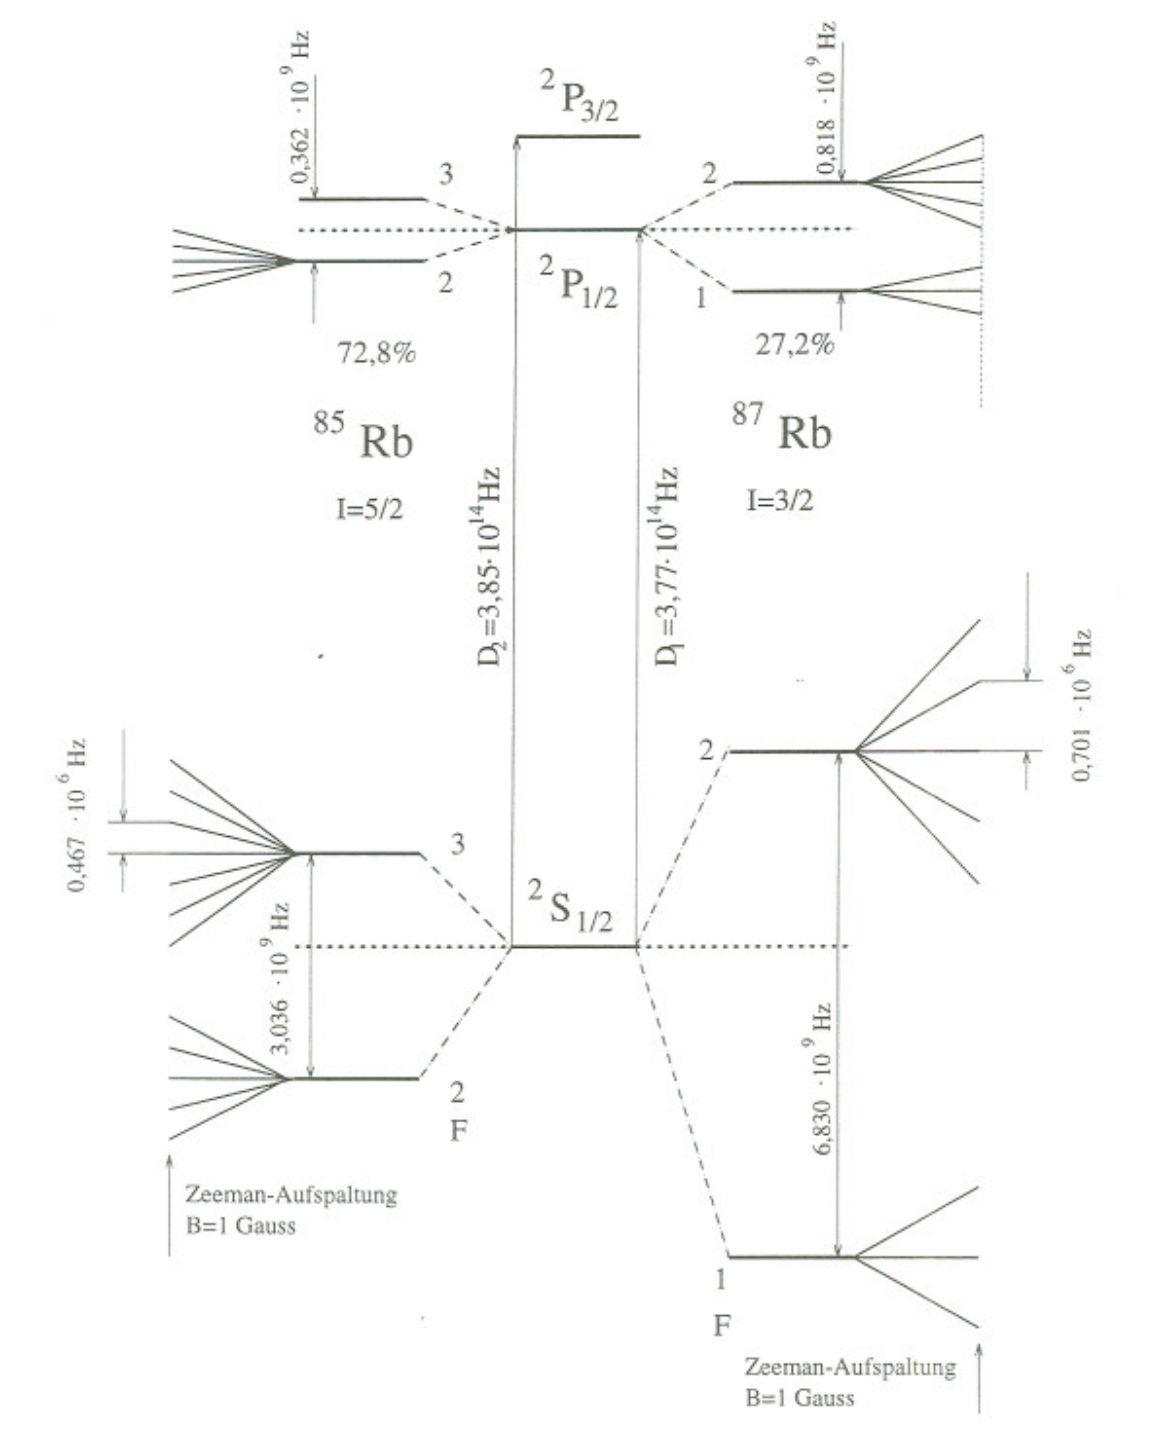
\includegraphics[width=1.0\linewidth]{graphics/hyperfinestructure}
\caption[Hyperfine structure of Rubidium]{The hyperfine structure of the two isotopes of Rubidium used in the experiment. The hyperfine levels in turn are split due to the Zeeman effect caused by an external field of $B=1$ G. \cite{staatsex}}
\label{fig:hyperfinestructure}
\end{figure}

\begin{figure}[H]
\centering
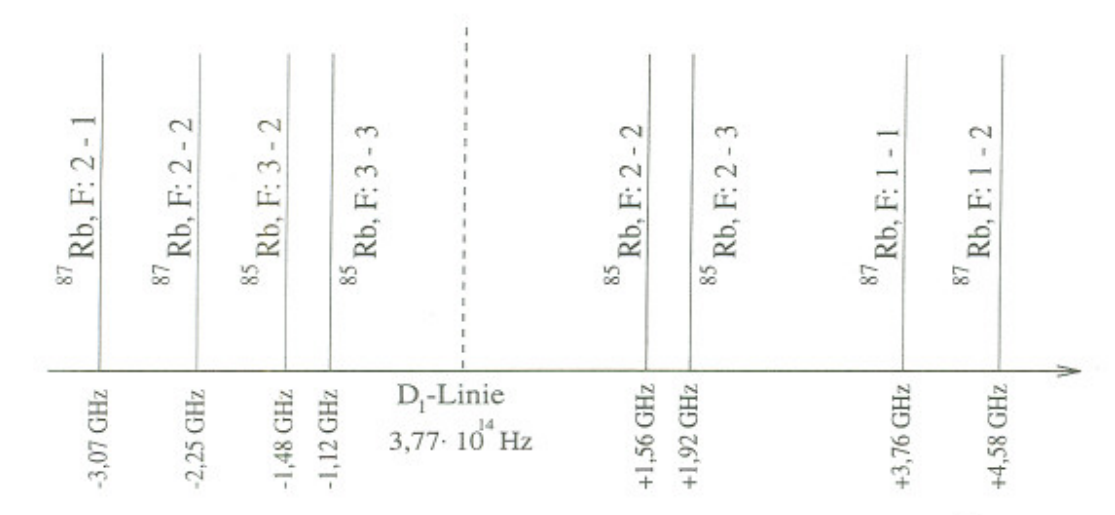
\includegraphics[width=1.0\linewidth]{graphics/hfslevels}
\caption[Hyperfine structure energies]{Energies of a set of hyperfine levels of the two isotopes used in the experiment. \cite{staatsex}}
\label{fig:hfslevels}
\end{figure}

These hyperfine levels can in turn be split into $2(F+1)$ sub-levels in the presence of an external magnetic field. The according quantum number is $-F\le m_F\le F$. As long as the magnetic field is weaker than the spin-orbit coupling or, in other terms, $g_J\mu_BB_0\ll A$, this is called the Zeeman effect. The effect for larger fields, where the spin-orbit coupling is disrupted, is called Paschen-Back effect.\\
For the Zeeman effect, the energy difference of the levels is
\begin{equation}
\Delta E_{Zeeman}=\frac{g_J}{2(I+\frac{1}{2})}\mu_BB_0
\label{eq:zeemanlevels}
\end{equation}

\subsection{Optical pumping}
In general, pumping refers to constantly transferring electrons into higher energy levels until significantly more electrons are in the higher than in the lower state. This is called population inversion.\\
In the case of this experiment, this is done using a laser diode. As the goal is to examine magnetic fields using the Zeeman splitting, a way must be found to create population inversion within a single non-degenerate hyperfine structure level. Normally, electrons are equally distributed between said levels.\\
The selection rules for transitions
\begin{equation}
\begin{aligned}
\Delta F&=0,\pm 1 \qquad (F=0\nleftrightarrow F=0)\\
\Delta m_F&=0,\pm 1
\end{aligned}
\end{equation}

allow for a convenient way to change that. If only $\sigma^+$-polarized light is used, only transitions with $\Delta m_F=+1$ are caused. Since the following decay is random within the bounds of the transition rules, the laser will pump all electrons into the $^2S_{1/2}$ state with $m_F=+2$, $F=2$ for $^{87}Rb$ and $m_F=+3$, $F=3$ for $^{85}Rb$. Figure \ref{fig:zeemanpumping} illustrates this for two exemplary transitions.\\
Mathematically, this process can be described as 
\begin{equation}
\left(\frac{dn}{dt}\right)_P=\frac{N-n}{T_P}
\label{eq:pumpingtime}
\end{equation}
where $n$ is difference of the levels in the two-level system, $N$ the overall number of atoms in the system and $T_P$ the characteristic pumping time of the system.
\begin{figure}[h]
\centering
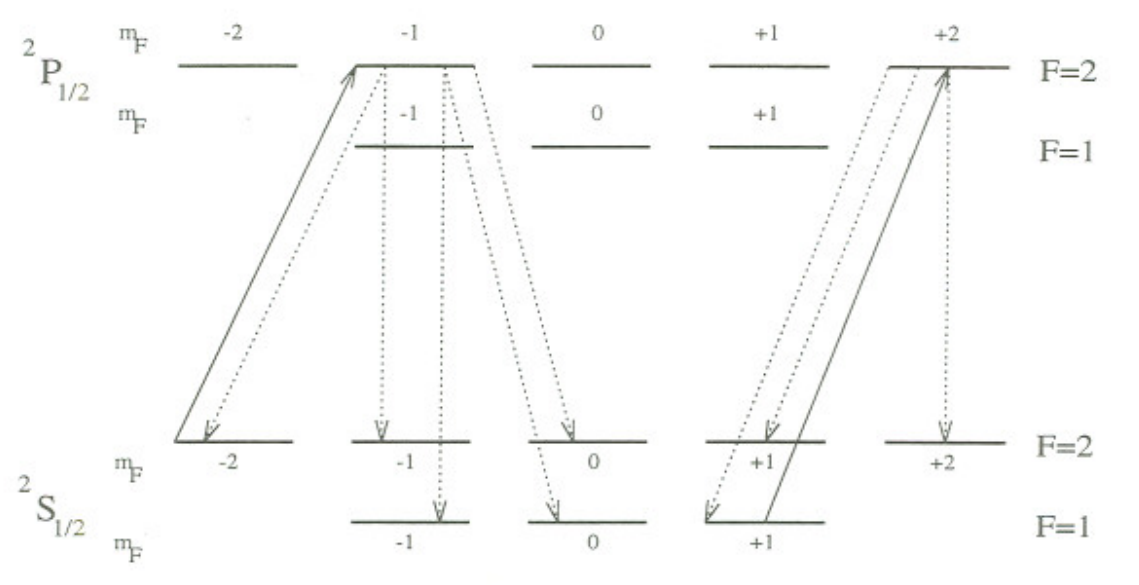
\includegraphics[width=1.0\linewidth]{graphics/zeemanpumping}
\caption[Optical pumping]{Optical pumping for $^{87}Rb$. The $\sigma^+$ polarized light can only cause transitions with $\Delta m_F=+1$, thus achieving the desired pumping effect.}
\label{fig:zeemanpumping}
\end{figure}
\subsection{Relaxation processes}
The desired pumping effect is counteracted mainly by three relaxation effects:
\paragraph{Diffusion to the wall:}
Upon hitting the glass containment, the rubidium atoms may lose their polarization. This process is inhibited by a buffer gas, which limits the mean free path of the atoms.
\paragraph{Collisions with the buffer gas:}
The rubidium atoms may use their polarization due to collisions with the buffer gas. The cross section of this event depend highly on what kind of gas is used. Best results are achieved with noble gases - in the case of this experiment, krypton was used.
\paragraph{Spin exchange}
When rubidium atoms collide, they may interchange their spins. While the overall polarization is preserved, the decoupling of nuclear and electron spins lead to a faster relaxation time. Much more detailed elaborations can be found in \cite{happer}.\\

Overall, the relaxation can be described by the following differential equation
\begin{equation}
\left(\frac{dn}{dt}\right)_R=-\frac{n}{T_R}
\label{eq:relaxationtime}
\end{equation}
where $T_R$ is the characteristic relaxation time. A value of $T^{theo}_R=6.5$ ms is given in \cite{staatsex}. The overall process of polarization orientation is thus the sum of equations \ref{eq:pumpingtime} and \ref{eq:relaxationtime}:
\begin{equation}
\left(\frac{dn}{dt}\right)_O=\left(\frac{dn}{dt}\right)_P+\left(\frac{dn}{dt}\right)_R=\frac{N}{T_P}-n\left(\frac{1}{T_P}+\frac{1}{T_R}\right)
\end{equation}

The solution of this equation is an exponential
\begin{equation}
n(t)\propto e^{-\frac{t}{\tau}}
\label{eq:orientationexponential}
\end{equation}

where $\tau=\frac{1}{T_P}+\frac{1}{T_R}$.
\subsection{Larmor precession of the spin}

\subsection{The laser diode}

\newpage
\section{Experimental set-up}
\begin{figure}[h]
\centering
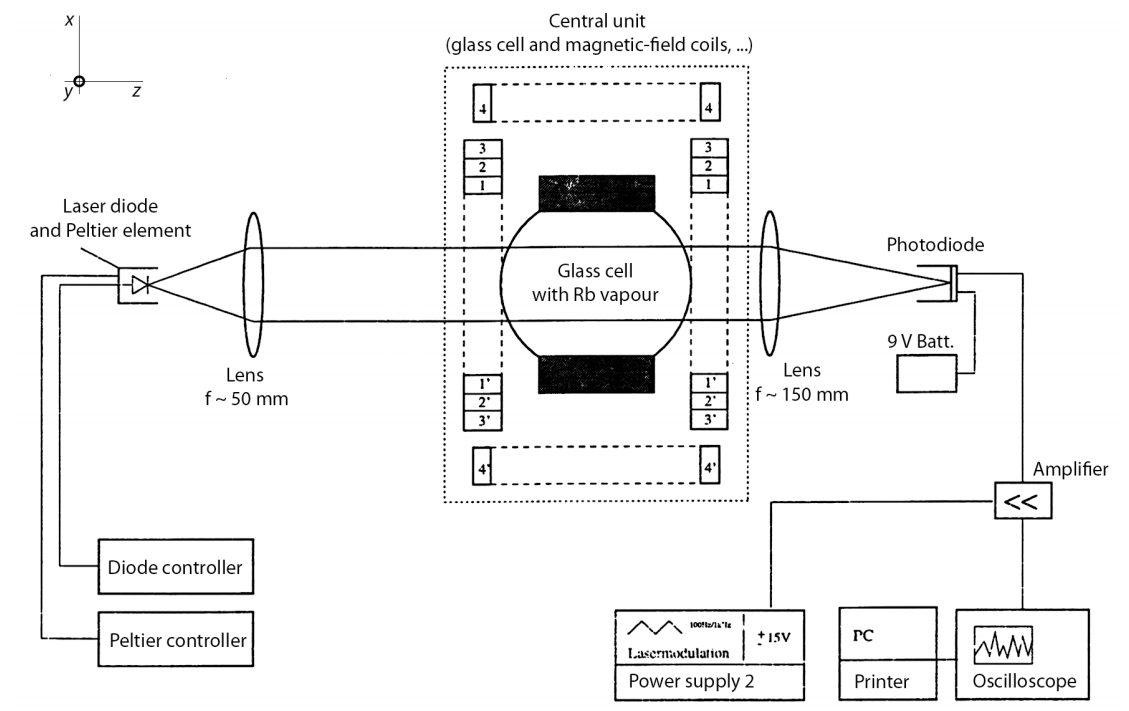
\includegraphics[width=1.0\linewidth]{graphics/generalsetup}
\caption[Basic experimental set-up]{Basic set-up of the experiment. For the various tasks, parts can be placed onto the optical bench. The glass cell can be removed from the central unit. \cite{anleitung} (modified)}
\label{fig:general setup}
\end{figure}
At the core of the experimental set-up is the glass cell with the Rubidium vapor and the buffer gas. It can be taken in and out of the central unit, which in turn houses four sets of Helmholtz coils. Another such pair is directly attached to the casing of the glass cell, along with a radio frequency generator and and appropriate frequency measuring device.\\

\textbf{A laser diode} provides coherent light in the energy range needed to pump the desired hyperfine state of the Rubidium atoms in the glass cell. Laser diodes send out linearly polarized light with a small spectral width. Frequency and intensity vary with the temperature of the diode as well as the current running through it, which is why the diode is kept at constant temperature using a Peltier element. For the diode to start emitting light, a certain current threshold has to be reached. From then on, the intensity depends linearly on the current if temperature is kept constant. However, mode jumps at certain currents disturb the linearity. Mode jumps occur when the number of standing waves in the resonator changes and measurements need to be taken in areas that do not include such jumps.\\

The beam is collimated by a lens before passing through other optical elements and, after passing through the central unit, is refocused onto a photo-diode. This can be seen in figure \ref{fig:general setup}. The output of the diode is amplified and can then be observed on an oscilloscope, which in turn can be read out by a computer to produce analyzable data.\\ 

The set-up varies greatly from one part of the experiment to another and will thus be explained in detail in the appropriate sections.


\section{Characterization of the laser diode}
For later measurements, it is important to determine the range of supply current in which the diodes intensity increases linearly without mode jumps occuring. The gas cell is taken out of the central unit for this part of the experiment. \\

After turning on the peltier element, a few minutes should pass before measurements are started to allow the diode to thermalize. Measurements were taken at $T=\unit{34.3}{\degree}$.\\
Since the photo diode saturated for laser diode currents upwards of $I_L=\unit{65}{mA}$, a neutral filter (D2,6, see figure \ref{fig:filterintensities}) is used to limit intensity so that the photo diode barely does not reach saturation.

The intensity of the diode is now measured at supply currents between $\unit{0-90}{mA}$. The results can be seen in figure \ref{fig:characterization}. The threshold current is roughly $\unit{51.6}{mA}$, followed by the linear domain until mode jump occur at around $\unit{72}{mA}$ to $\unit{82}{mA}$. 
\begin{figure}[htb]
\centering
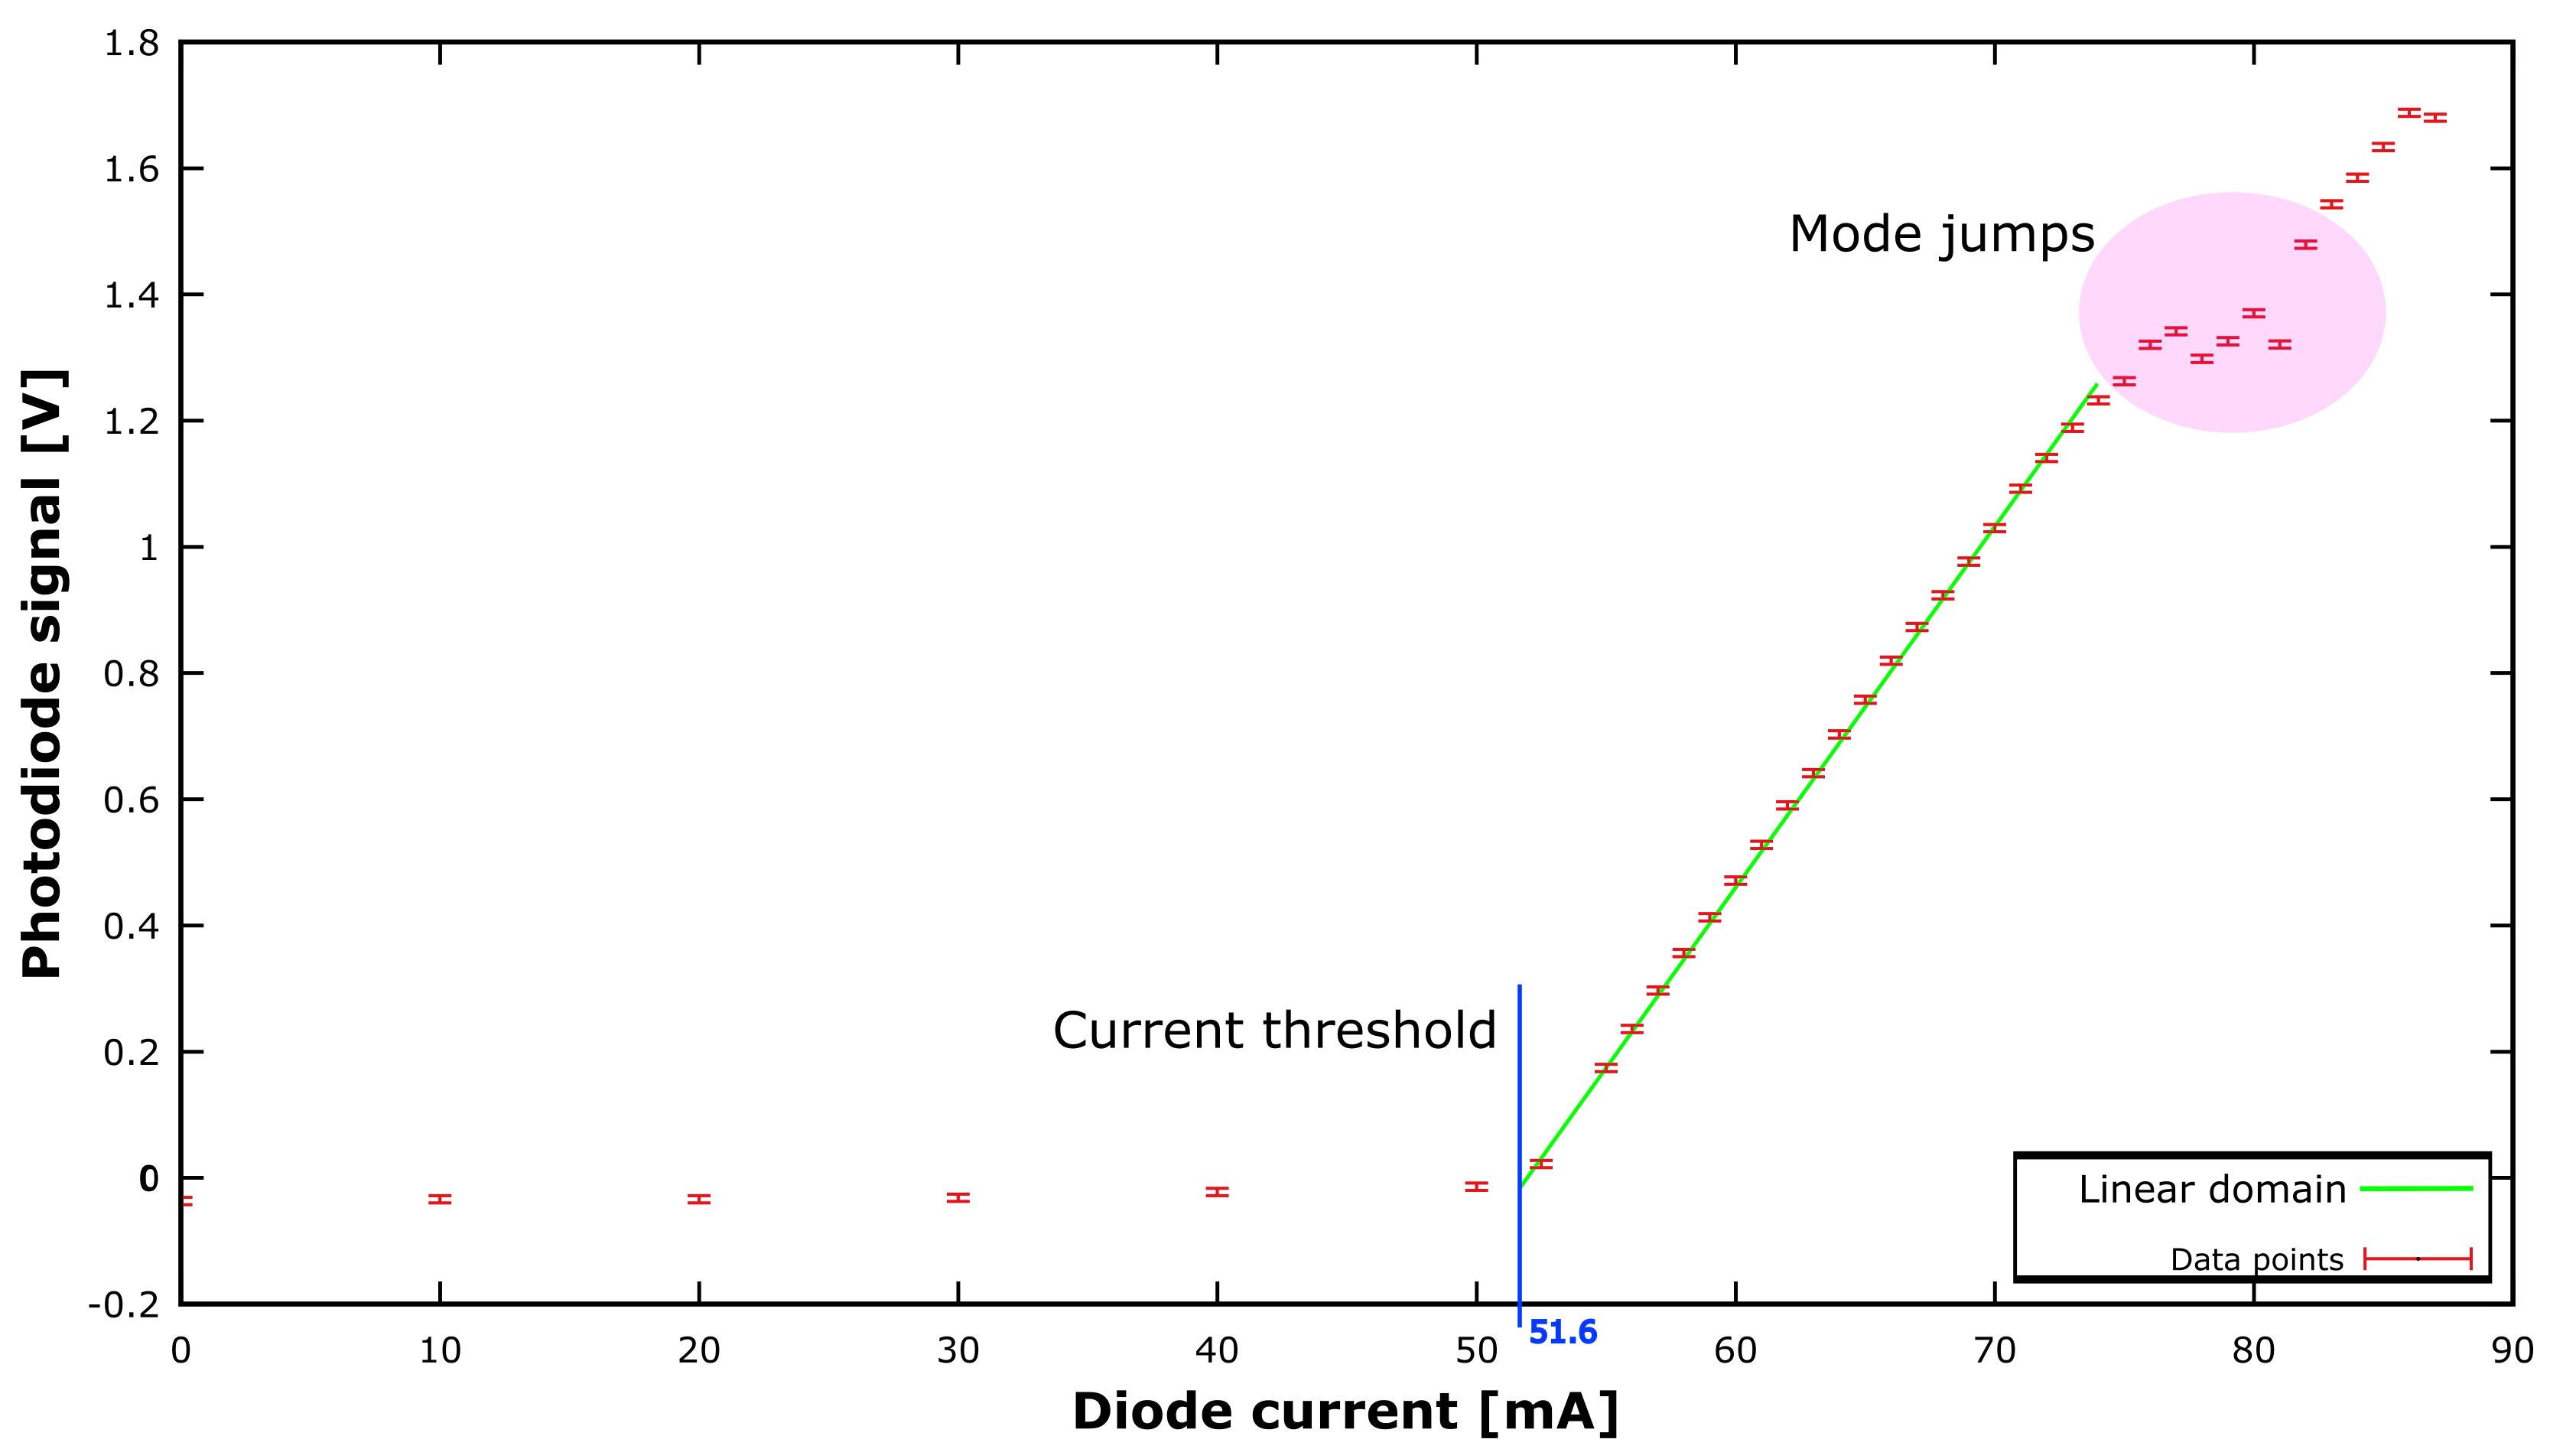
\includegraphics[width=1.0\linewidth]{graphics/characterization}
\caption[Characteristic curve of the laser diode]{The characteristic curve of the laser diode for supply currents up to $\unit{90}{mA}$. A mode jump can clearly be seen in the uper right corner.}
\label{fig:characterization}
\end{figure}







\section{Spectroscopy of the hyperfine structure}
\subsection{Set-up and procedure}
\begin{figure}[htb]
	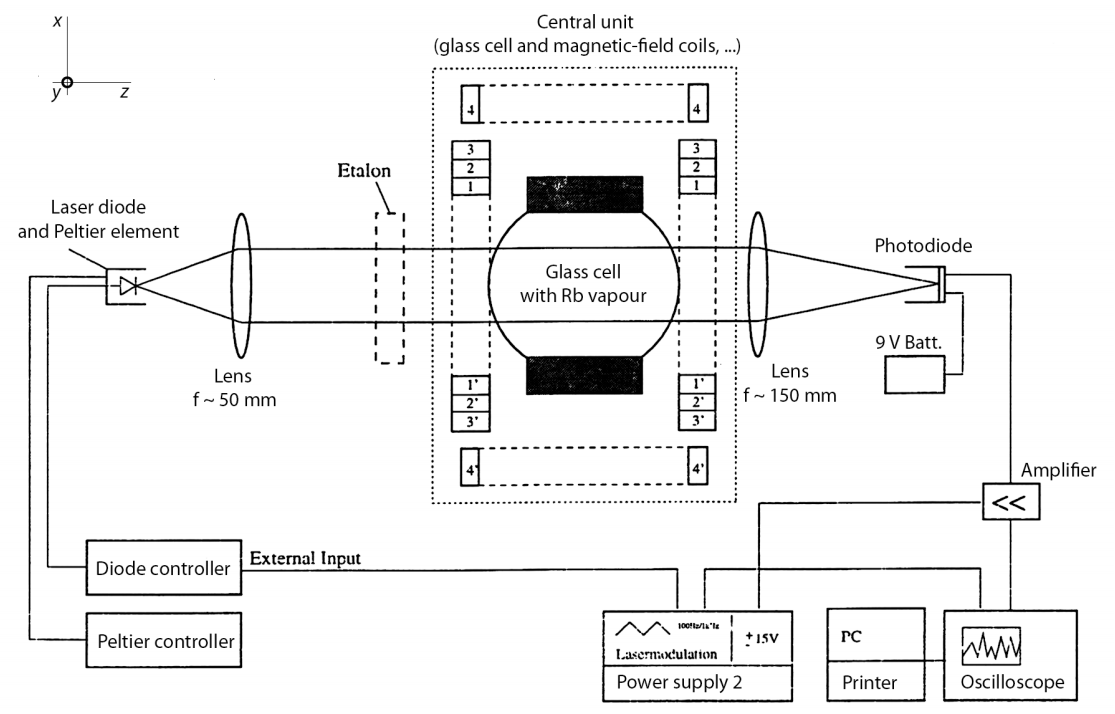
\includegraphics[width=1.0\linewidth]{graphics/calibrationsetup}
	\caption[Experimental set-up for the Calibration]{Experimental set-up for the calibration measurements. An etalon is placed after the left lens and can be removed for the HFS-spectrum measurement.\cite{anleitung}}
	\label{fig:calibration setup}
\end{figure}
\subsubsection*{Laser scan-rate}
A Fabry-Pérot-Interferometer (etalon), which is a set of parallel, almost completely reflecting surfaces facing each other, is used to gauge the diode. The intensity at the photo diode will be drastically dampened unless the laser wavelength allows for constructive interference to occur between the surfaces. The wavelengths at which light passes the interferometer are thus equidistant.\\

The diode current is then modified with a saw-tooth voltage, which is also used to trigger the oscilloscope(see figure \ref{fig:calibration setup}). It is important to measure the scan-rate in a range of diode currents where the intensity response is linear and where the HFS-spectrum is actually visible (see next section). To get a solid calibration, at the very least 3 etalon peaks are necessary. These two factors have to be taken into consideration when choosing the measurement interval.\\ 

Figure \ref{fig:bendincurve} shows a bend in the diode current. Such areas need to be avoided when taking measurements, as they would lead to non-equidistant peaks in the etalon spectrum and unnecessarily complicate data analysis.
\begin{figure}
	\centering
	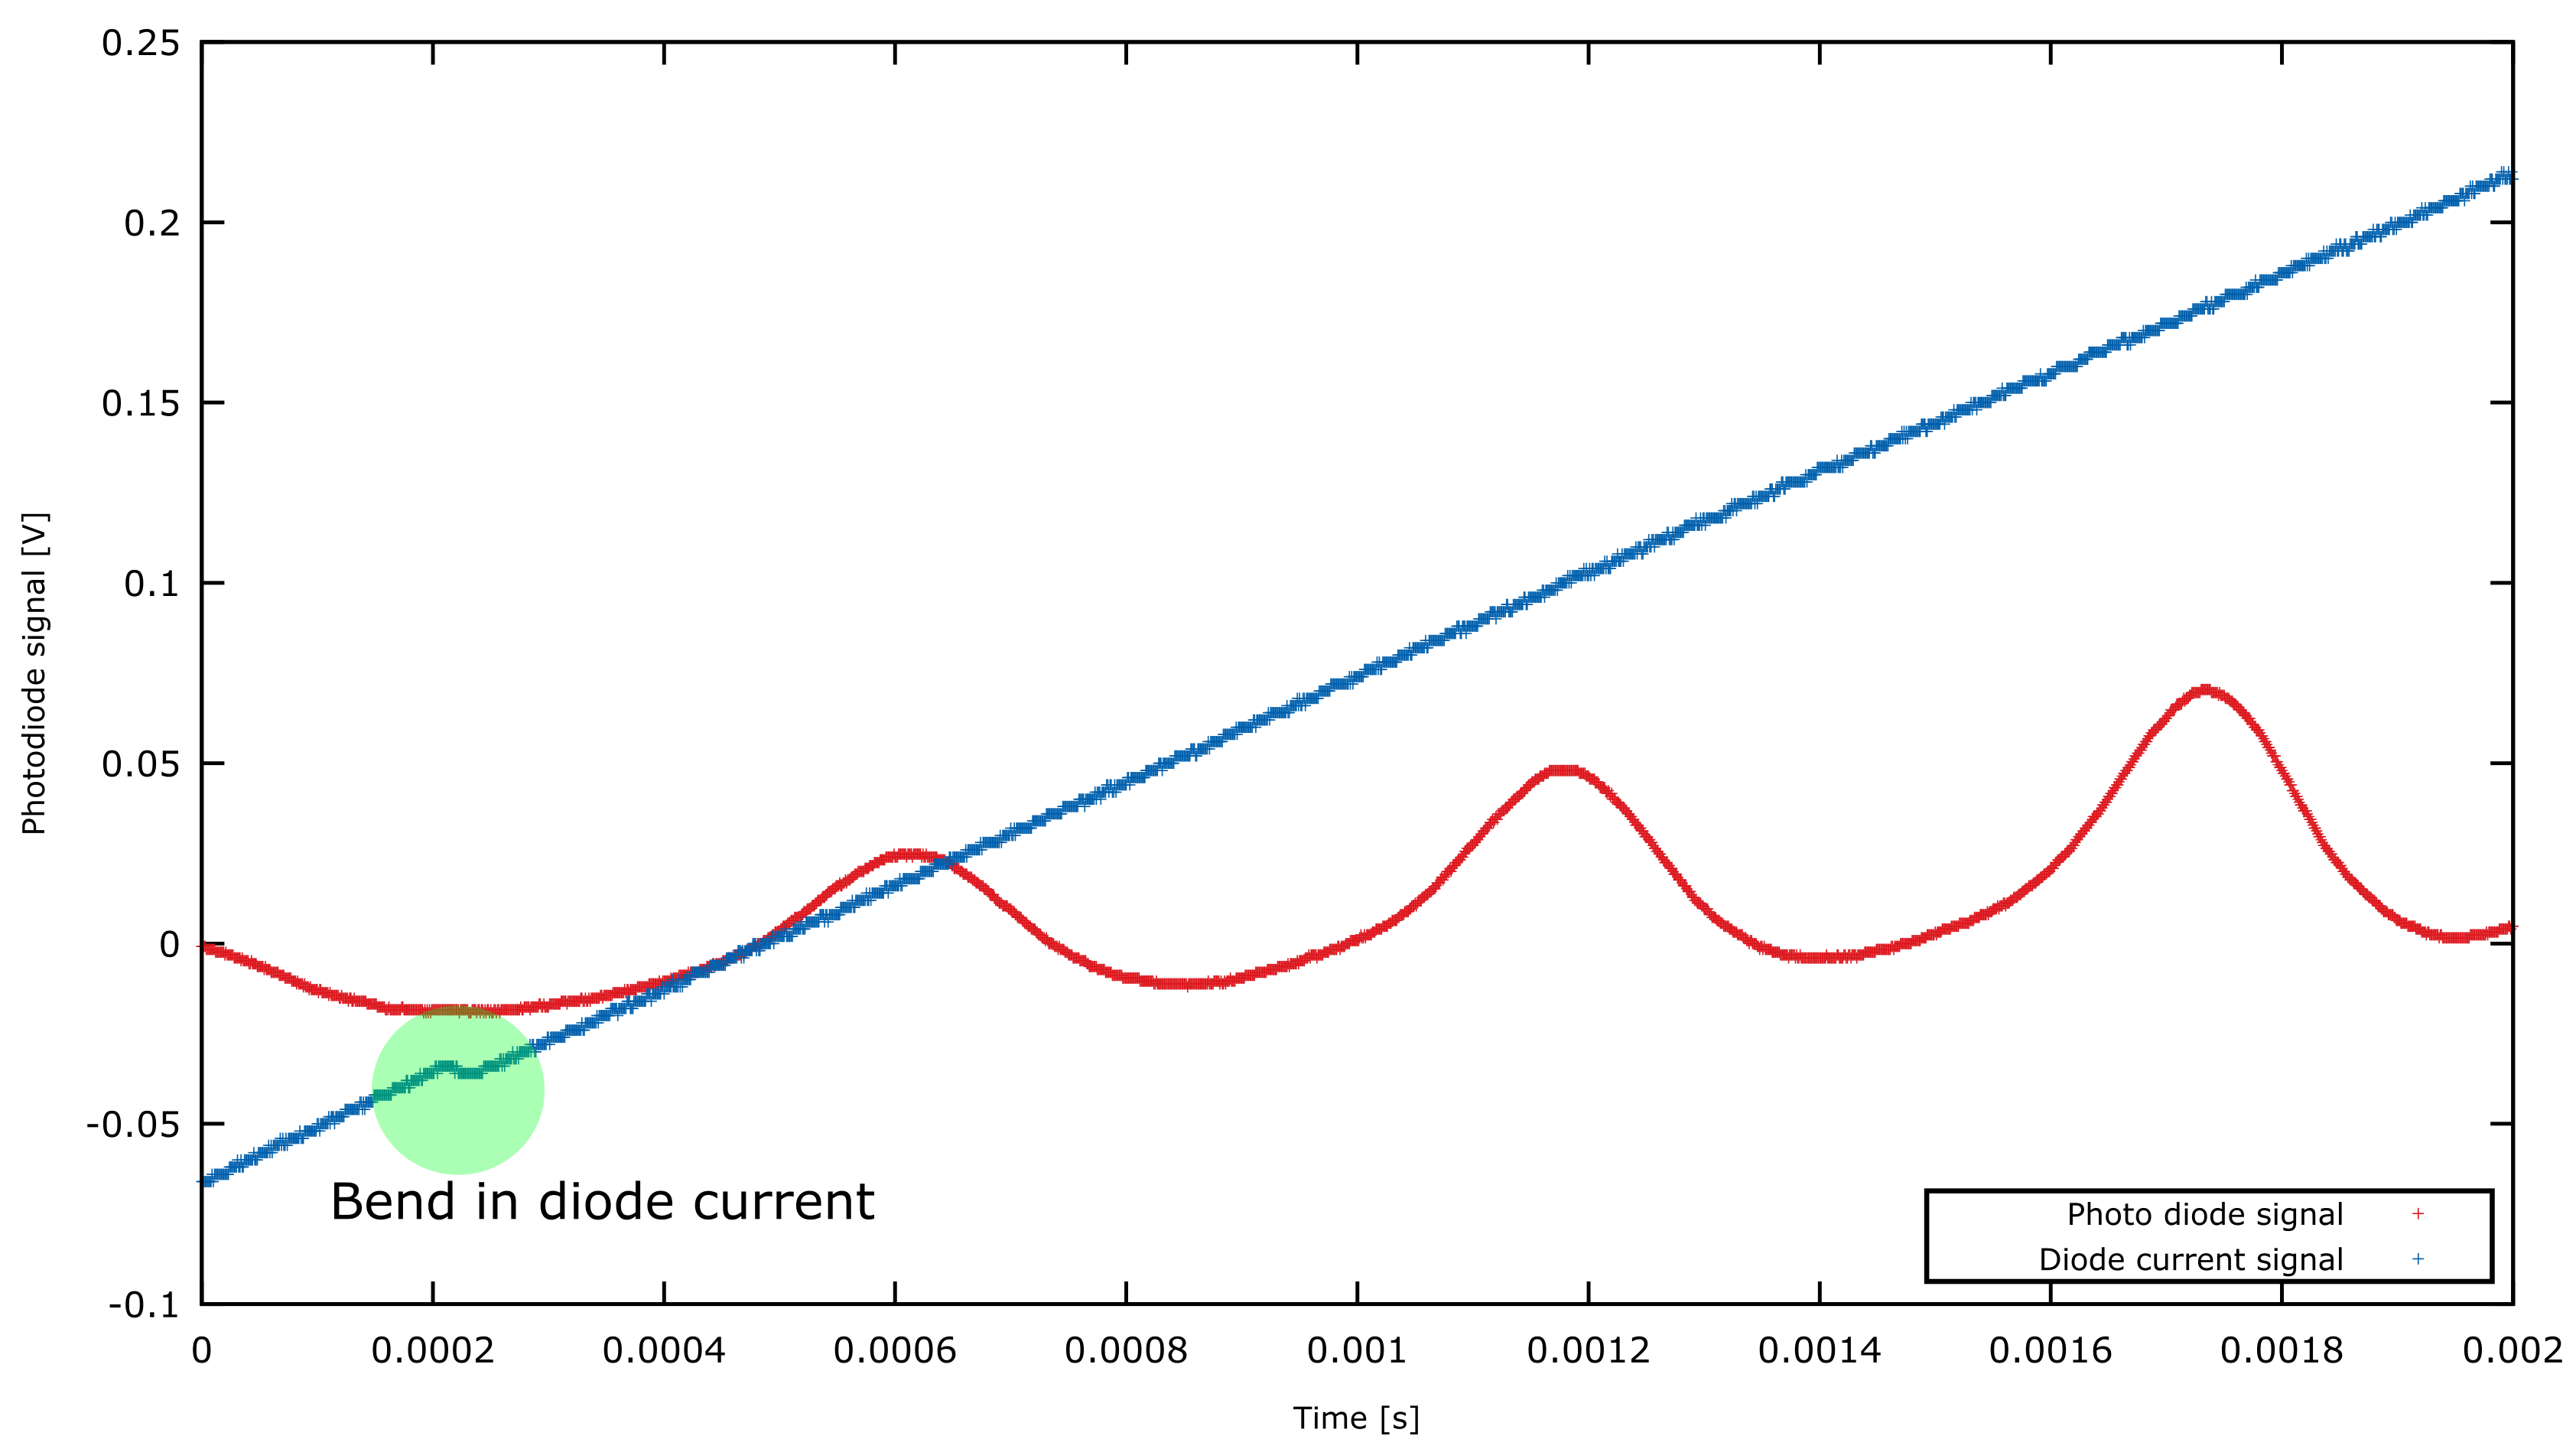
\includegraphics[width=1.0\linewidth]{graphics/bendincurve}
	\caption[Bend in modulating current]{In the bottom left corner, a clear bent in the diode current can be seen. These measurements were not used, a better current range was chosen instead.}
	\label{fig:bendincurve}
\end{figure}
The base current for the measurements was $I_L=\unit{(58.5\pm0.1)}{mA}$, where the uncertainty is the digit error of the multimeter ELTELEC, for which no data sheet was available. The temperature remained at $T=\unit{34.3}{\degree}$. The resulting intensity distribution can be seen in figure \ref{fig:etalon_fit}.

\subsubsection*{The HFS-spectrum}
The etalon is removed for this measurement and the exact same current modulation of the laser current as has been used for the scan-rate measurements will be used here as well. As the intensity increases with increasing diode current, the spectrum would have a linear offset. This can be counteracted by inverting the photo diode signal and adding the diode current signal to it. An additional cosmetic advantage of this is that the peaks are then positive.


\subsection{Data analysis}
\subsubsection*{Laser scan rate}
\begin{figure}[htb]
\centering
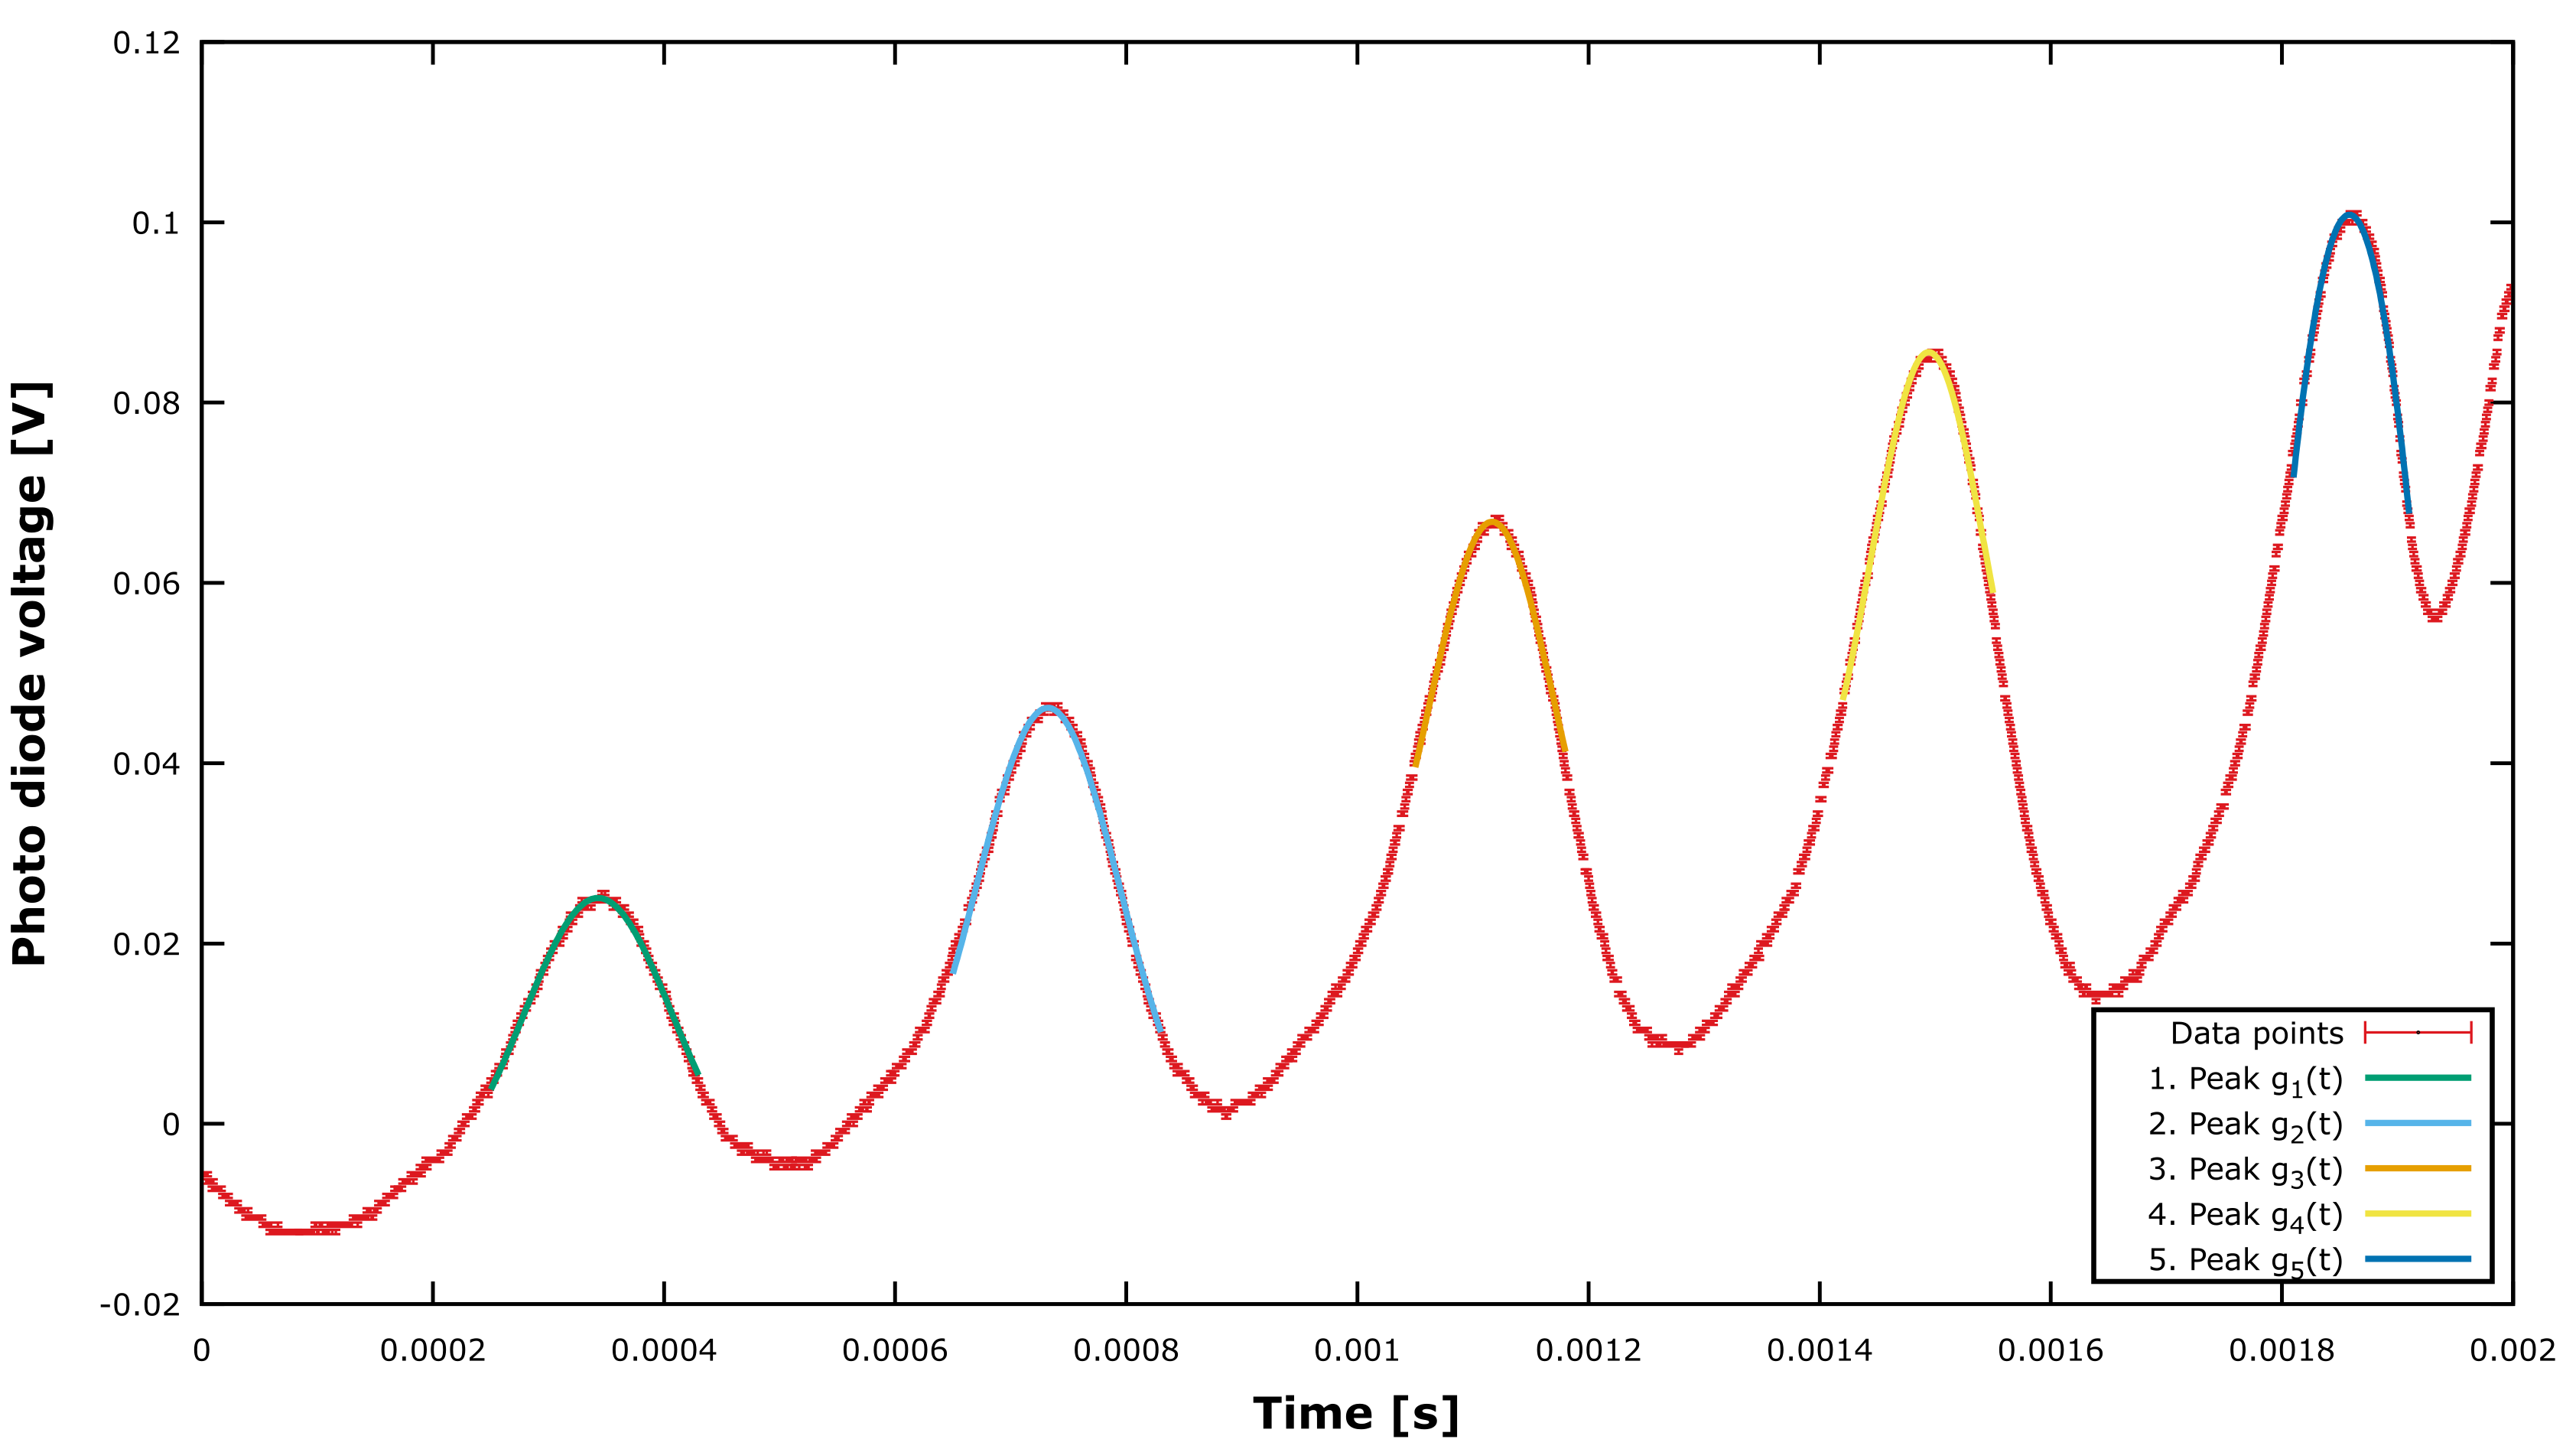
\includegraphics[width=1.0\linewidth]{graphics/etalon_fit}
\caption[Etalon peaks]{Results of the etalon calibration measurements. The rightmost peak is actually the same as the one on the left of it, as the saw-tooth reaches its peak between the two.}
\label{fig:etalon_fit}
\end{figure}
In figure \ref{fig:etalon_fit}, it has to be noted that the saw-tooth voltage reaches its maximum between the rightmost peak and the one on the left of it, meaning that these two actually belong to the same frequency. The rightmost peak is thus ignored for the calibration.\\
Gauss functions with a constant offset of the form
\begin{equation}
	g_i(t)=a_i*e^{-\frac{(t-t_{0,i})^2}{2*\sigma_i^2}}+c_i
	\label{eq:gaussfit}
\end{equation}
and a linear offset function $l(t)=b*t+c$ were used. 
The results for the peak positions $t_{0,i}$ can be seen in figure \ref{fig:ethalon_linearfit}. As the linear fit shows, these peaks are equidistant as expected with the time distance between peaks being $b=\unit{(0.379\pm0.003)}{ms}$. The nominal distance between two peaks is $\Delta_{FSR}=\unit{(9924\pm30)}{MHz}$. With these two values, the scan rate $r$ of the laser can be calculated as
\begin{equation}
	r=\unit{(26.17\pm 0.22)}{\frac{GHz}{ms}}
\end{equation}

\begin{figure}[htb]
\centering
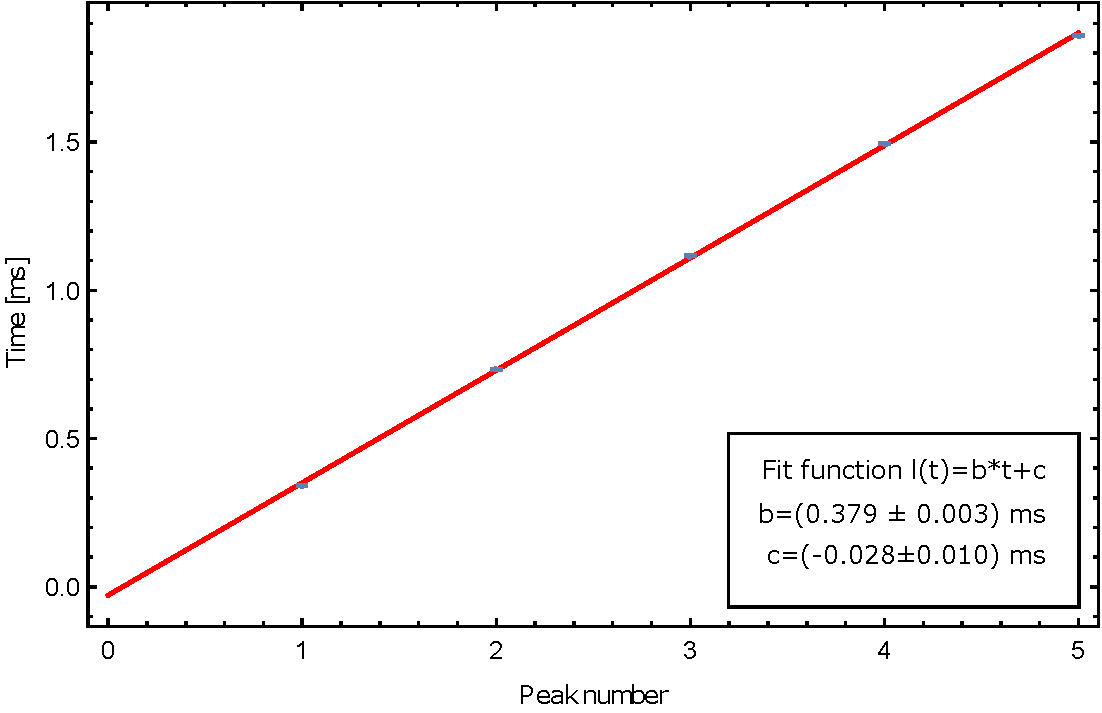
\includegraphics[width=1.0\linewidth]{graphics/ethalon_linearfit}
\caption[Lienear fit on etalon peak positions]{Linear fit on the etalon peak positions.}
\label{fig:ethalon_linearfit}
\end{figure}

\subsubsection*{HFS-spectrum}
Only 6 of the expected 8 peaks (see figure \ref{fig:hfslevels}) are visibly separated here. It is reasonable to assume that the peaks that were not separable are those of the transitions $^{85}$Rb F:3-2 and $^{85}$Rb F:3-3 as well as $^{85}$Rb F:2-2 and $^{85}$Rb F:2-3. This also means that the hyperfine constant for the $^2S_{\nicefrac{1}{2}}$ of $^{85}$Rb cannot be calculated with these measurements.
Gauss functions like those in equation \ref{eq:gaussfit} were used for the individual peaks. However, for the peaks that overlap, as sum of the two functions was used. For all fits, both a linear function and a constant were added and the total sum fitted to the data. The fit function for the last three peaks for example was
\begin{equation}
I_{4-6}(t)=g_4(t)+g_5(t)+g_6(t)+b\cdot t+c
\end{equation}
Table \ref{tb:HFSresults} lists the result of the fits as well as the frequency distances to the reference peak, which was arbitrarily chosen to be the first peak.
\begin{table}\centering
	\begin{tabular}{@{}lllllll@{}}
		\toprule
		&Peak No &$t_0$ [ms]&$s_{t_0}$ $\unit{}{[\micro s]}$ & &$\tau^+\tau^-$&Transition\\
		\midrule
		&1&0.104&0.18&&&$^{87}$Rb F:1-2\\
		&2&0.129&0.92&&&$^{87}$Rb F:1-1\\
		&3&0.215&0.05&&&$^{85}$Rb F:2-2/3\\
		&4&0.340&0.03&&&$^{85}$Rb F:3-2/3\\
		&5&0.371&0.06&&&$^{87}$Rb F:2-2\\
		&6&0.399&0.06&&&$^{87}$Rb F:2-1\\	
		\bottomrule
	\end{tabular}
	\caption[HFS peaks fit results]{Fit results of the Gauss fits on the HFS spectrum. The frequency calibration was used to calculate the differences to the reference peak.}
	\label{tb:HFSresults}
\end{table}


\begin{figure}[htb]
	\centering
	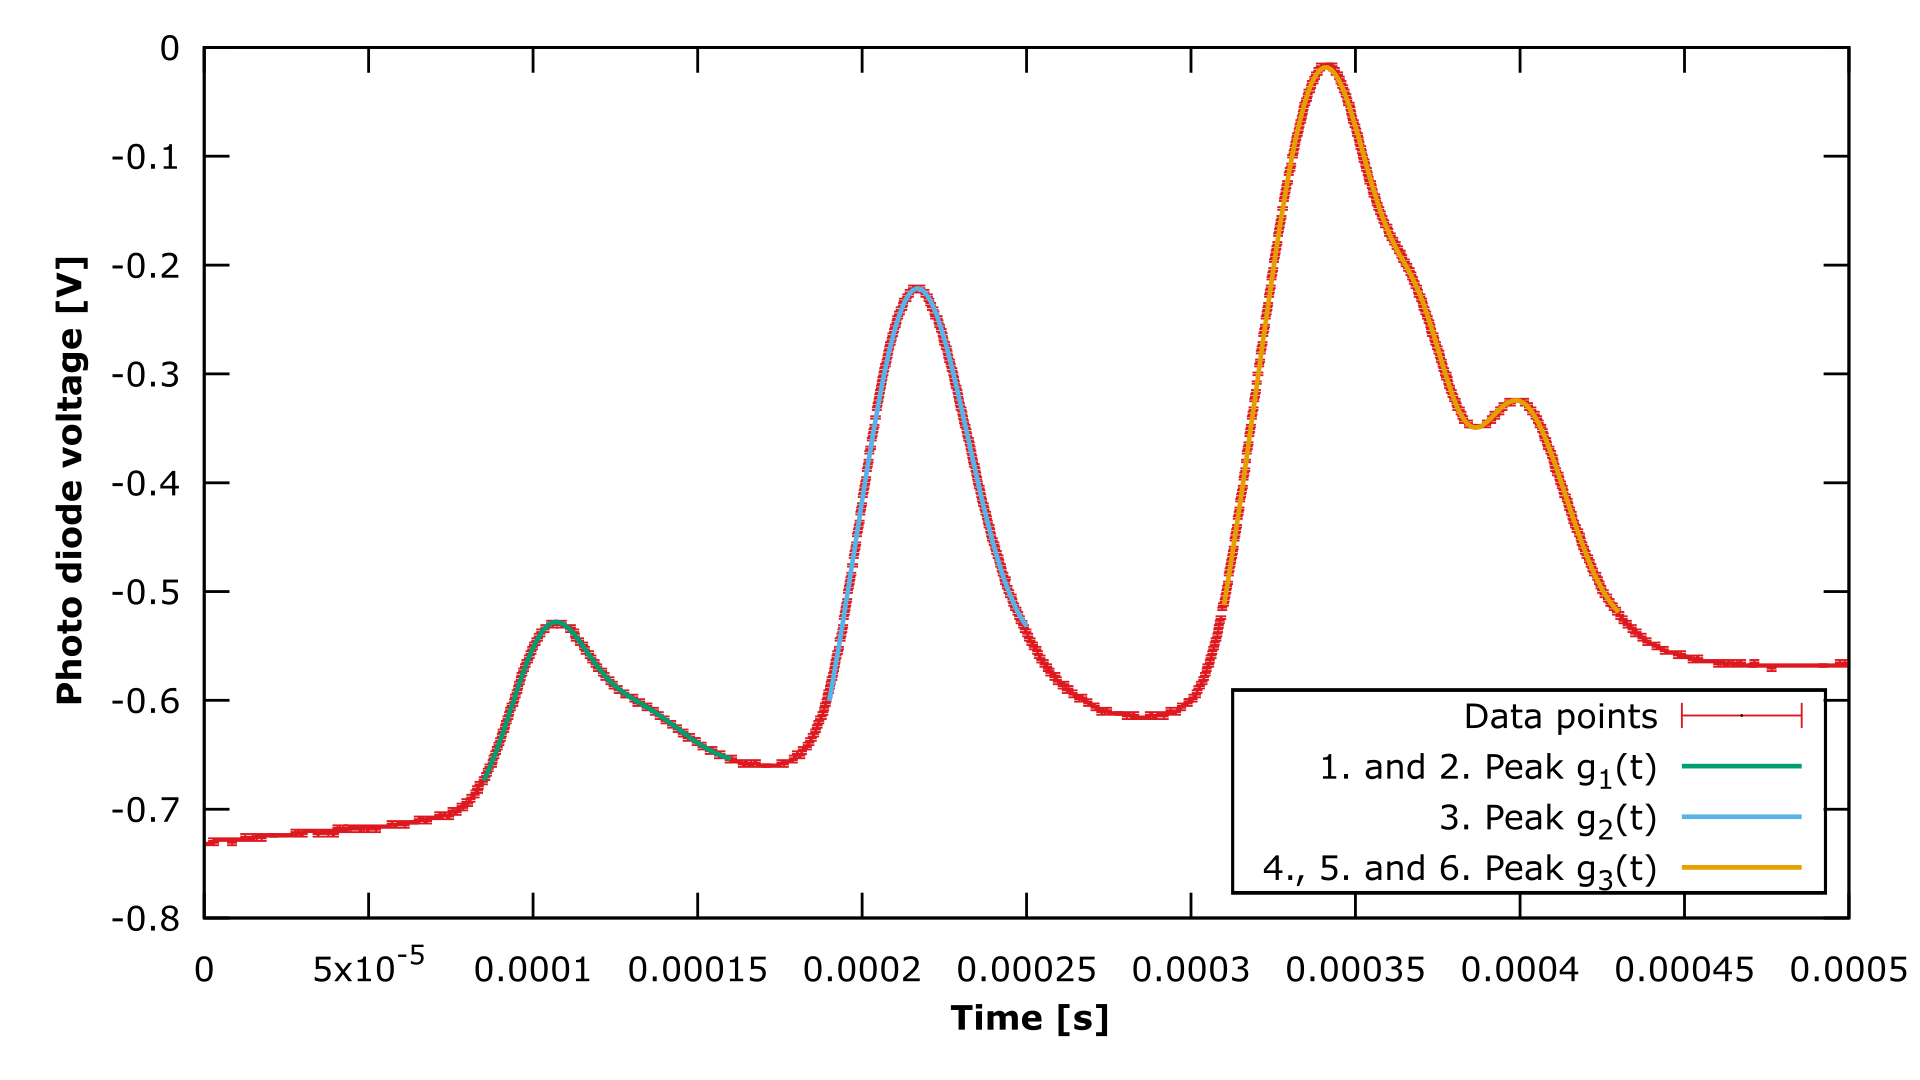
\includegraphics[width=1.0\linewidth]{graphics/HFS_fits}
	\caption[The HFS-spectrum]{The HFS-spectrum with fits to the individual peaks. The signal is negative since it was inverted.}
	\label{fig:HFS_fits}
\end{figure}



\newpage
\section{Double resonance}
\subsection{Set-up and procedure}
\begin{figure}[htb]
\centering
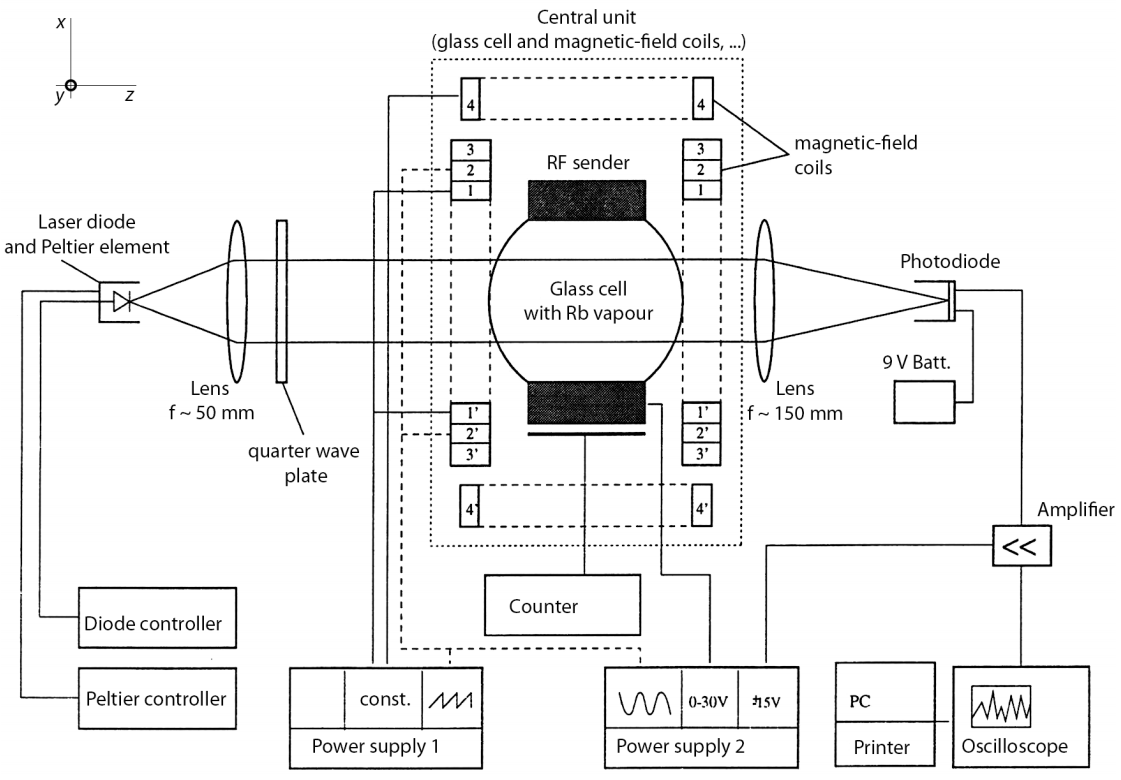
\includegraphics[width=1.0\linewidth]{graphics/doubleresonancesetup}
\caption[Double resonance set-up]{Experimental set-up for the double resonance measurements.\cite{anleitung}}
\label{fig:doubleresonancesetup}
\end{figure}
This measurement is called double resonance since we both pump the Zeeman states and, at the same time, depopulate the polarized state with radio frequency radiation (RF radiation from here on). Both effects can be described as a resonance. The RF frequency can be measured with a frequency counter which is also built into the glass cell unit.  The glass cell is now always lodged in the central unit.\\
To achieve pumping, the polarization of the laser light needs to be changed from linear to circular. It does not matter where it is right or left circular - that merely changes the direction of polarization. To achieve circular polarization, a quarter wave plate is used. As the polarization after said place depends on the angle of the linear polarization of the incident light, one has to check whether the light is actually circularly polarized after the wave plate. For that, a linear polarizer is used to check whether or not the intensity signal varies upon turning the linear polarizer, which it should not.\\ 
A sinusoid current is run through coil 2 (see fig. \ref{fig:doubleresonancesetup}), at first with a large amplitude to find the magnetic field range for which double resonance occurs. Once the range is determined, a constant current is applied to coil 1. The double resonance peaks are now visible, but Dehmelt peaks, which are a result of relaxation once the magnetic field crosses zero, are still visible. It can easily be determined which is which, as the double resonance peaks disappear when one turns off the RF generator. For the Dehmelt peaks to disappear, the amplitude of the sinusoid in current two has to be reduced so that the overall magnetic field does not cross zero anymore.  Coil 4, which creates a field along the x-axis in figure \ref{fig:doubleresonancesetup}, can now be used to compensate the vertical magnetic field of the earth. When it is compensated, the negative peaks should have maximal depths. The current through coil 4 is then kept at this value for the main measurement.\\
With the vertical magnetic field compensated, the current in coil 1 can now be tuned to make the two peaks per period equidistant. In this state, the magnetic field from coil 1 stretches the Zeeman spectrum exactly enough for the RF frequency to relax the polarization. One such value must exist for both current directions through coil 1. This is done for both rubidium isotopes. The laser current is measured with an exterior multimeter, since the digital display is on has a precision of $\unit{1}{mA}$. From these four values, the longitudinal magnetic field of the earth can be measured and the nuclear spins $I$ of th isotopes calculated.

\subsection{Data analysis}
\begin{figure}
\centering
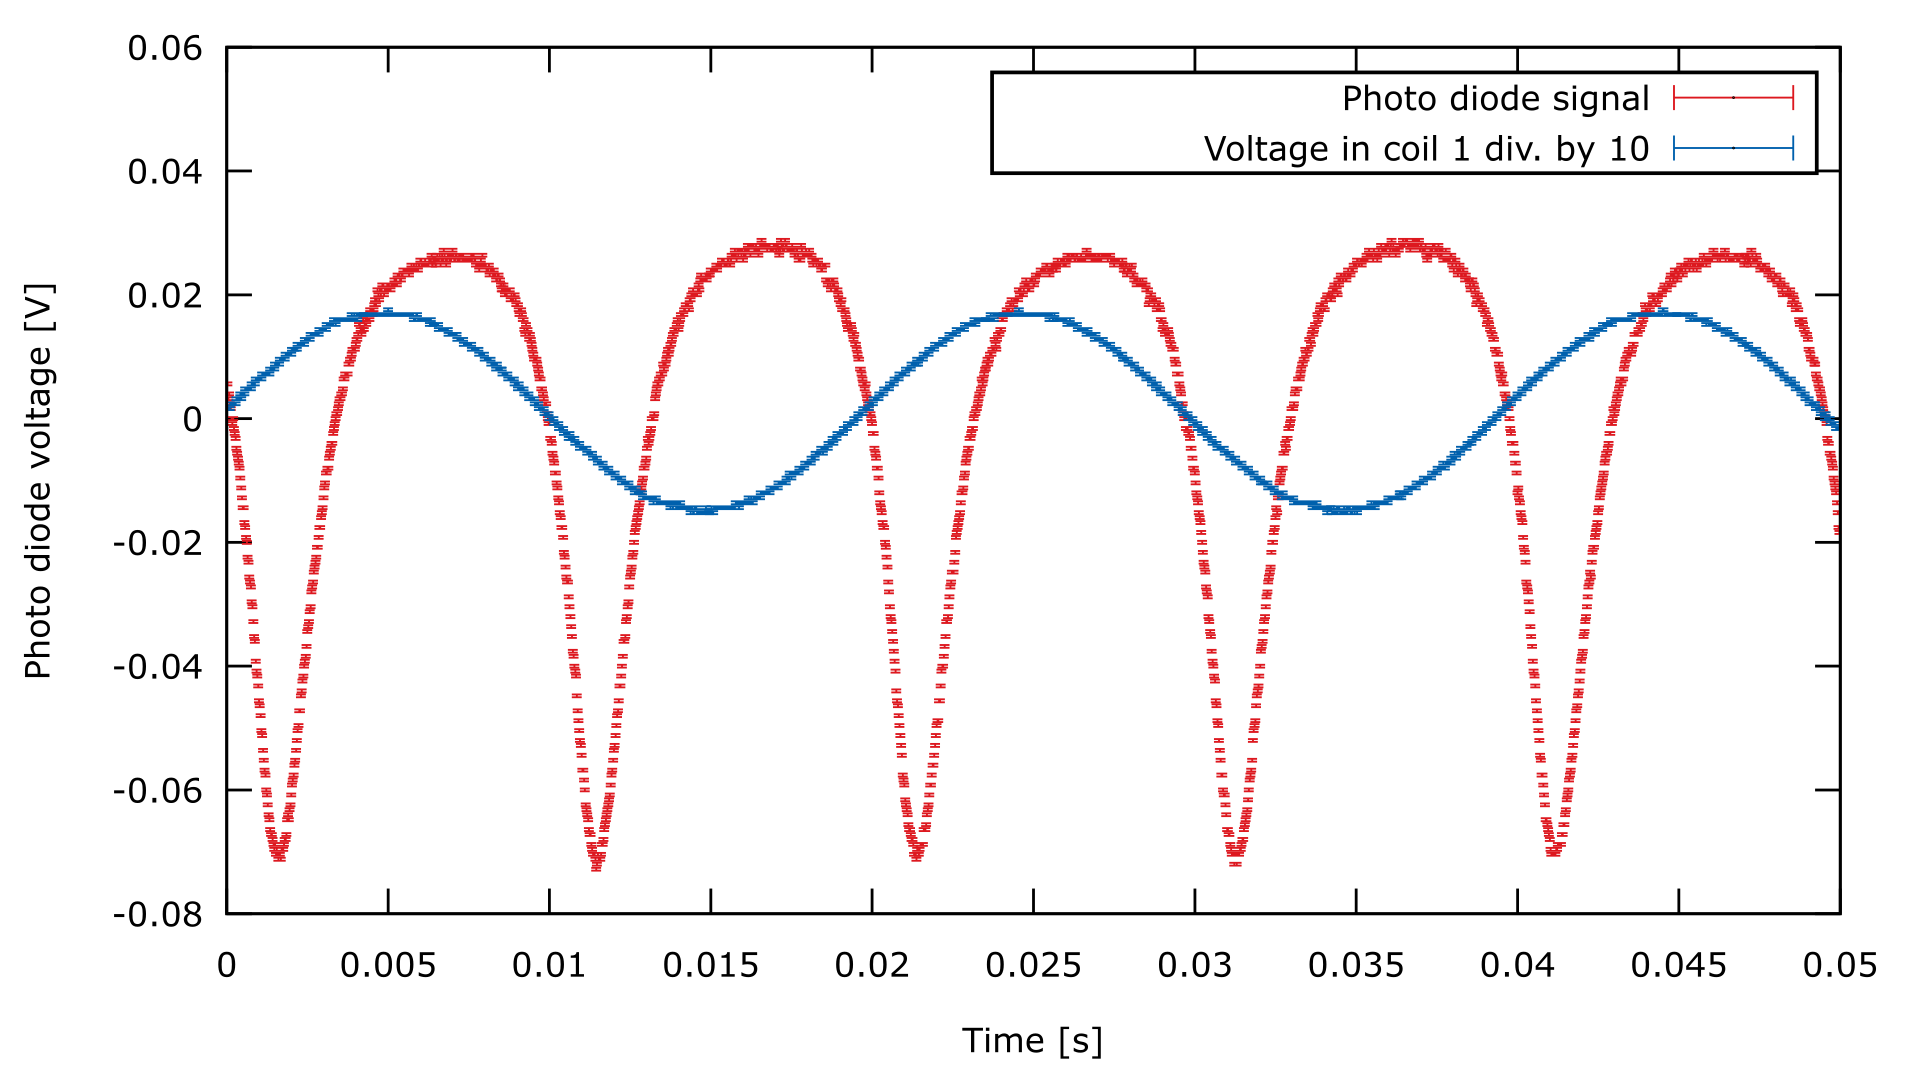
\includegraphics[width=1.0\linewidth]{graphics/equaldistance}
\caption[Double resonance peaks]{Equidistant peaks for $I_L=\unit{61.8}{mA}$ and a current in coil 1 of $I_{C1}=\unit{130.2}{mA}$. Note the phase shift: The double resonance peaks do not occur at the zero-crossing of the coil voltage, but at those of the coil current. The coil voltage was divided by ten to make the photo diode signal more dominant.}
\label{fig:equaldistance}
\end{figure}
Measurements were taken at $T=\unit{34.4}{\degree}$ and with a RF frequency of $\nu_{RF}=\unit{(497\pm1)\cdot10^3}{Hz}$. An uncertainty of $s_{I_{C1}}=\unit{0.5}{mA}$ was estimated for current at which the peaks are equidistant. The results can be seen in table \ref{tb:doubleresonance}. The current in coil 4 for which the vertical field was compensated was determined to be $I_{C4}=\unit{(78\pm3)}{mA}$.\\
The constants $c_B=B/I$ of the coils in table \ref{tb:coilconstants} were provided for the calculations of the magnetic fields that the coils create.

\begin{table}\centering
	\begin{tabular}{@{}llllll@{}}
		\toprule
		&Coil No&n &d [m]&calc. $\unit{B/I}{[\frac{Vs}{Am^2}]}$&meas. $\unit{B/I}{[\frac{Vs}{Am^2}]}$]\\ 
		\midrule
		&1&80&0.09&$8.0\cdot10^{-4}$&$7.99(1)\cdot10^{-4}$\\
		&2&80&0.09&$8.0\cdot10^{-4}$&$8.14(1)\cdot10^{-4}$\\
		&3&16&0.09&$1.7\cdot10^{-4}$&--\\
		&4&60&0.246&$4.4\cdot10^{-4}$&$4.76(1)\cdot10^{-4}$\\
		\bottomrule
	\end{tabular}
	\caption[Properties of the magnetic field coils]{The $B/I$ values and properties of the Helmholtz coils. $n$ is the number of windings. \cite{anleitung}}
	\label{tb:coilconstants}
\end{table}
The magnetic fields are
\begin{equation}
B=c_b\cdot I_C,\qquad s_B=\sqrt{(c_b\cdot s_{I_C})^2+(I_C\cdot s_{c_b})^2}
\end{equation}
where $I_C$ is the current in the respective coil. Table \ref{tb:doubleresonance} lists those results for coil 1. From the current in coil 4, the vertical magnetic field was calculated to be
\begin{equation}
B_v=\unit{(37.1\pm1.4)}{\micro T}
\end{equation}
\begin{table}\centering
	\begin{tabular}{@{}lllllll@{}}
		\toprule
		&$I_L$ [mA]&$s_{I_L}$ [mA]&$I_{C1}$	[mA]&$s_{I_{C1}}$ [mA]&$B_{C1}$ [\micro T]&$s_{B_{C1}}$ [\micro T]\\ 
		\midrule
		&62.4&0.1&91.2&0.5&71&10\\
		&62.4&0.1&-85.3&0.5&85&9\\
		&61.8&0.1&136.1&0.5&109&12\\
		&61.8&0.1&-130.2&0.5&104&11\\
		\bottomrule
	\end{tabular}
	\caption[Results of the double resonance measurements]{The results of the double resonance measurements. The magnetic field signs were matched with those of the currents.}
	\label{tb:doubleresonance}
\end{table}
The magnetic fields are all written with positive sign. Let $B_1$ be the magnetic field of the positive, $B_1'$ the negative coil current. The horizontal component of the earths' magnetic field is equal to half the difference of these two fields
\begin{equation}
B_h=\frac{B_1-B_1'}{2},\qquad s_{B_h}=\frac{1}{2}\cdot\sqrt{s_{B_1}^2+s_{B_1'}^2}
\end{equation}
The magnetic field difference is identical for the two isotopes, but the error is slightly different. The mean of the two is
\begin{equation}
B_h=\unit{(2.36\pm 0.21)}{\micro T}
\end{equation}
When calculating the mean value of $B_1$ and $B_1'$,
\begin{equation}
\overline{B}_1=\frac{B_1+B_1'}{2}
\end{equation}
the magnetic field component of the earth cancels out and yields the magnetic field that is responsible for the Zeeman splitting. Together with the frequency $\nu_{RF}$ and by using equation \ref{eq:zeemanlevels}, the nuclear spins $I$ of the two isotopes can be calculated as
\begin{equation}
I=\frac{\mu_B\cdot \overline{B}_1}{h\cdot\nu}-\frac{1}{2},\qquad s_I=\frac{\mu_B\cdot \overline{B}_1}{h\cdot\mu}
\sqrt{\left(\frac{s_{\overline{B}_1}}{\overline{B}_1}\right)^2
	+\left(\frac{s_\nu}{\nu}\right)^2}
\end{equation}
Since greater diode current corresponds to lower frequency and thus lower transition energy, the current $I_{C1}=\unit{62.4(1)}{mA}$ corresponds to $^{87}$Rb and the $I_{C1}=\unit{61.8(1)}{mA}$ to $^{85}$Rb. The results for the spins were
\begin{align}
	I(^{85}\text{Rb})&=2.496\pm0.009\\
	I(^{87}\text{Rb})&=1.486\pm0.007\\
\end{align}
\subsection{Discussion}
The literature values for the earths' magnetic field are \cite{anleitung}
\begin{equation}
B_v^{lit}=\unit{42.9}{\micro T}, \quad B_h^{lit}=\unit{20.9}{\micro T}
\end{equation}
while the measurements yielded $B_h=\unit{(2.36\pm 0.21)}{\micro T}$ and $B_v=\unit{(37.1\pm1.4)}{\micro T}$. While the result for the vertical field encloses the literature value in its $4\sigma$ interval, the result for the horizontal field is nowhere near the expected value. To double check the results, a Hall effect sensor was used. Since the sensor only had a resolution of $\unit{10}{\micro T}$, it only useful for qualitative analysis. These measurements revealed that not only is the horizontal field much weaker inside the metal casing of the experimental set-up, the experimental set-up is also not aligned with the projection of the magnetic field lines on its horizontal axis. Due to time constraints, the measurements could not be repeated with an aligned table. The deviation in the vertical field can likely be attributed to shielding effects of the building.\\

The calculated values for the spins are in good agreement, enclosing the expected values of $I(^{87})=\nicefrac{3}{2}$ in the $2\sigma$ interval and $I(^{85})=\nicefrac{5}{2}$ in the $1\sigma$ interval.

\newpage
\section{Spin precession}
\subsection{Set-up and procedure}
\begin{figure}
\centering
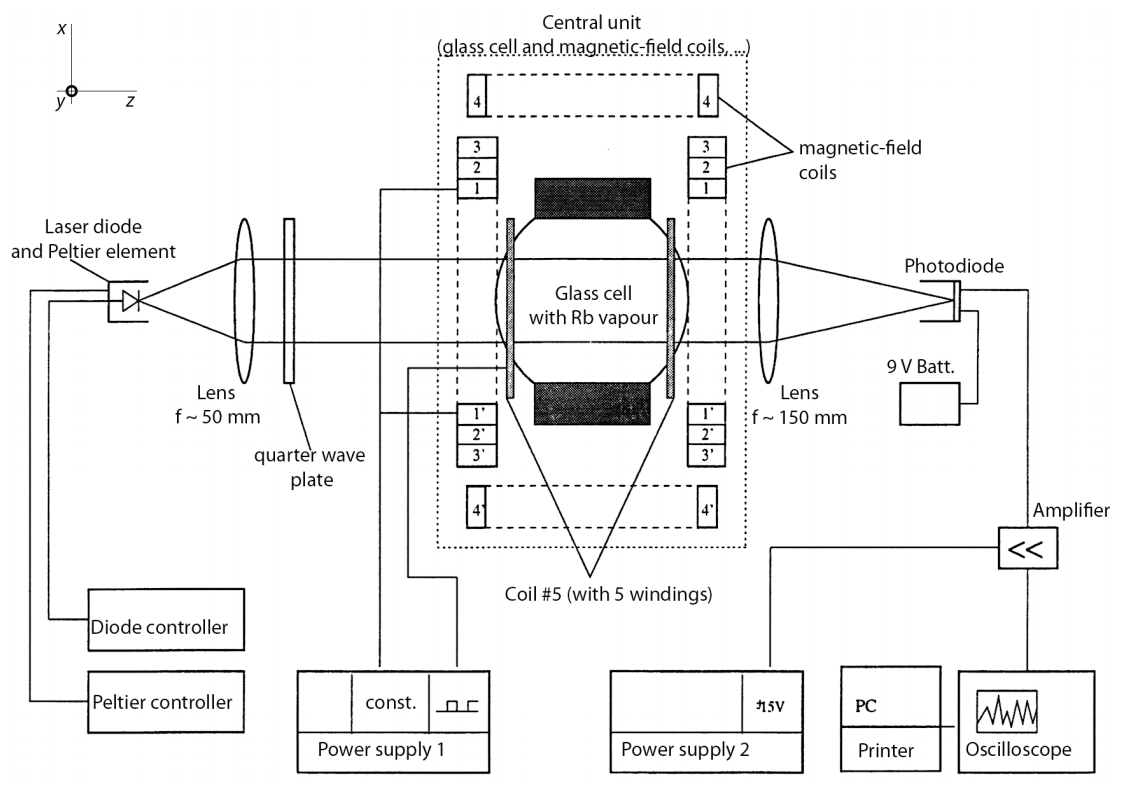
\includegraphics[width=1.0\linewidth]{graphics/spinprecessionsetup}
\caption[Spin precession set-up]{Experimental set-up for the spin precession measurements. \cite{anleitung}}
\label{fig:spinprecessionsetup}
\end{figure}
As before, only a quarter wave plate and the glass cell are placed in the beam. For the spin precession, the horizontal field as it was calculated in the double resonance section is compensated with a current in coil 1. A rectangular signal is given onto coil 5 so that the horizontal component of the magnetic field is compensated regularly. The spin precedes around the remaining vertical component, which can be varied by currents in coil 4. Measurements of the precession are then taken for a range of currents in coil 4.\\

Upon initial measurements, where both horizontal and vertical component were compensated as per the results from the double resonance section, it became clear that there was still a magnetic field, since precession could still be observed. As mentioned before, the table is not aligned with the horizontal component of the earths' magnetic field. Thus, the table was rotated until a minimal precession frequency was found. The degree by which the table was turned was by $\phi=\unit{(7\pm2)}{\degree}$ and measurements were then taken as described above.

\subsubsection{Analysis}
\begin{figure}
	\centering
	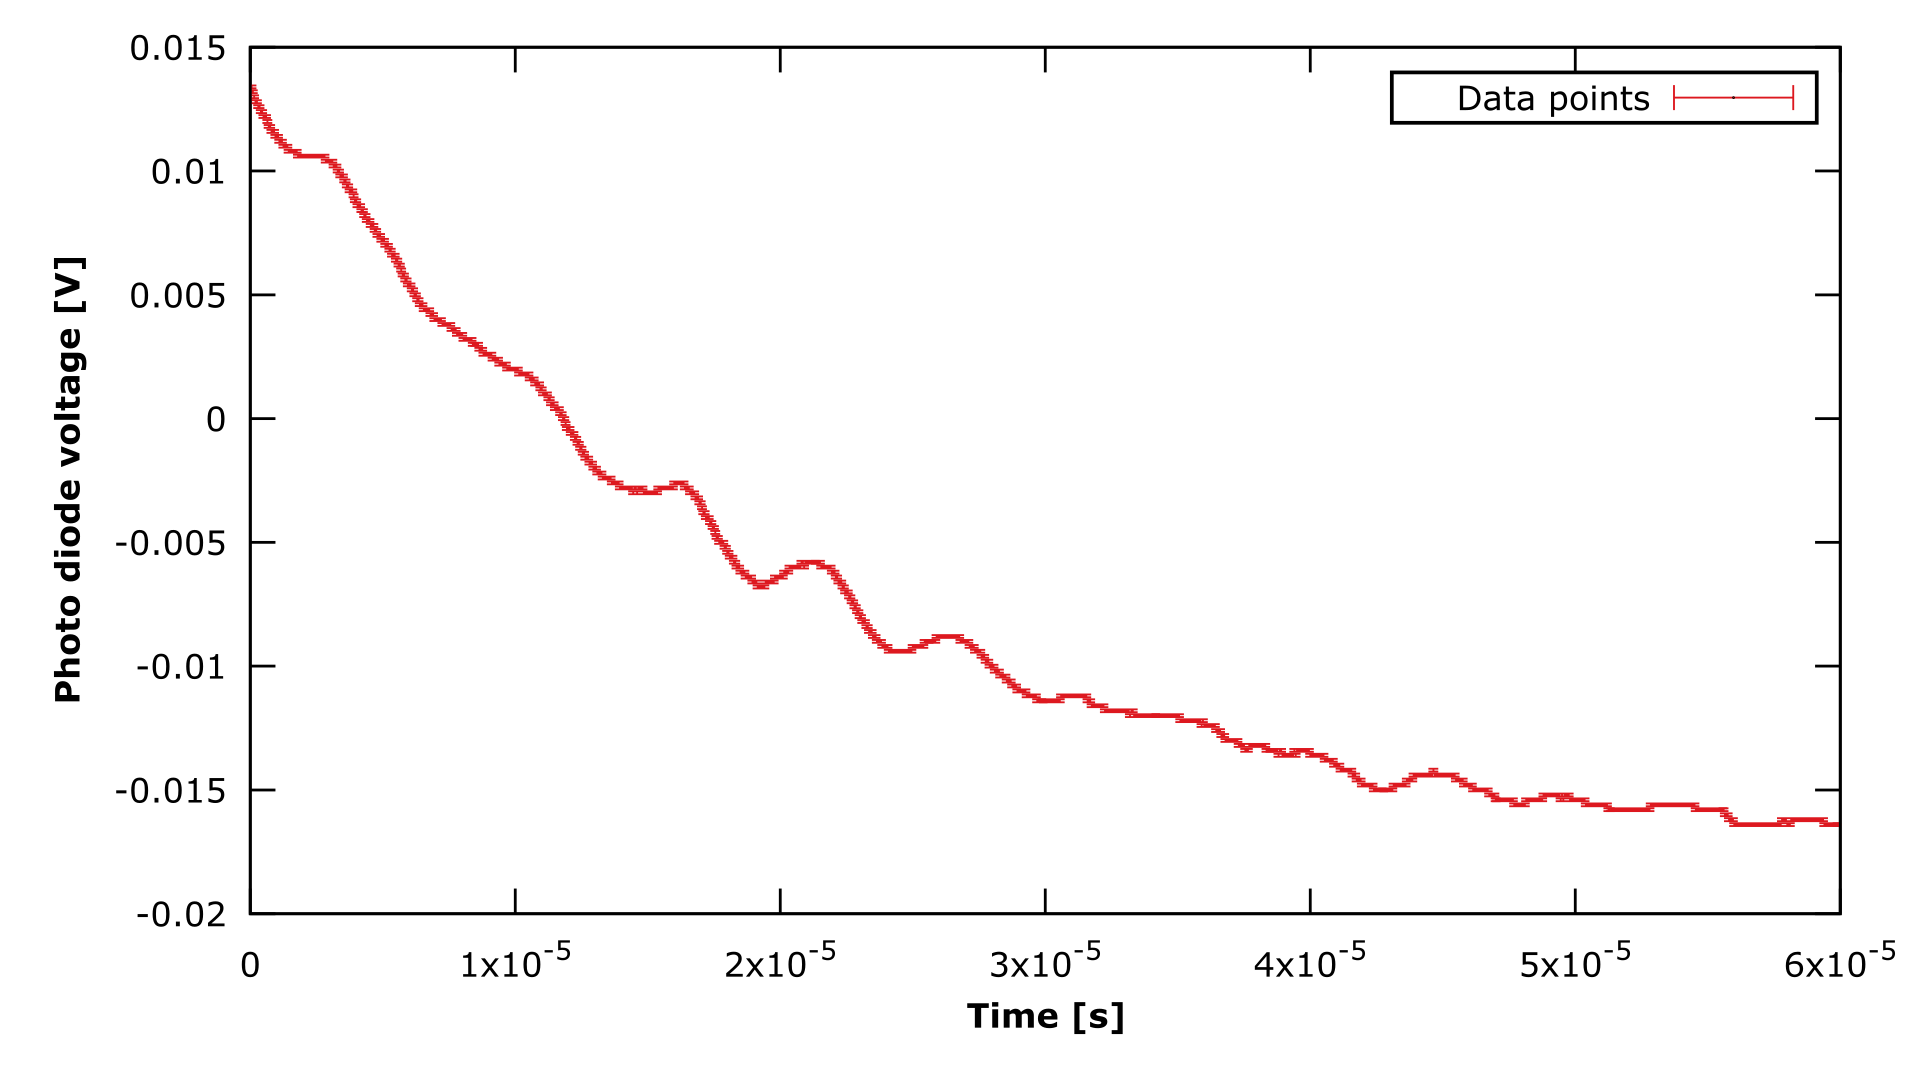
\includegraphics[width=1.0\linewidth]{graphics/spinprecessionexample}
	\caption[Example spin precession]{Examplary plot of the spin precession measurement. The peak positions were read off.}
	\label{fig:spinprecessionexample}
\end{figure}
Measurements were taken only for a diode current of $I_L=\unit{62.0}{mA}$, which was the current corresponding to $^{87}$Rb. No precession signal was found for $^{85}$Rb. The temperature during the measurements was $T=\unit{34.3}{\degree}$ and the current for the compensation of the horizontal field after turning the table was $I_{C1}=\unit{(6\pm1)}{mA}$.\\
The time differences between peaks were read out of appropriate sub plots of the recorded data. One exemplary plot can be seen in figure \ref{fig:spinprecessionexample} and all the values that were read out in table \ref{tb:precessionpeaks}. First, the time difference $\Delta t$ and its error were calculated
\begin{equation}
\Delta t=t_2-t_1, \qquad s_{\Delta t}=\sqrt{2}\cdot s_{t_{12}}
\end{equation}
where $s_{t_{12}}$ is the estimated error on reading the peaks as it is listed in table \ref{tb:precessionpeaks}.\\
There sometimes were no properly readable adjacent peaks. While it was always clear that there was a peak, it was much easier to read out the second most adjacent peak. Those values are marked with a star in the first column in table \ref{tb:precessionpeaks} and their time difference is
\begin{equation}
\Delta t=\frac{t_2-t_1}{2},\qquad s_{\Delta t}=\frac{1}{\sqrt{2}}s_{t_{12}}
\end{equation}
The precession frequency $\nu_L$ can now be calculated
\begin{equation}
\nu_L=\frac{1}{\Delta t},\qquad s_{\nu_L}=\frac{s_{\Delta t}}{(\Delta t)^2}
\end{equation}
and the results are plotted in figure \ref{fig:freqlinfit}. A linear fit $f(x)=a\cdot x+b$ was used to describe the data and the resulting parameters were $a=\unit{(-3.40\pm0.17)}{kHz/mA}$ and $b=\unit{(280\pm11)}{kHz}$ with $\chi^2=9.9$. One can extrapolate to the magnetic field for which the precession frequency would be zero, assuming that all other fields were actually compensated for. The current in coil 4 for said field is $I^0_{C4}=\frac{-b}{a}=\unit{(82\pm5)}{mA}$ and the according magnetic field $B_v=\unit{39.2\pm2.5}{\micro T}$. This is within $1\sigma$ of the value calculated in the double resonance section.\\
Since the magnetic field is reduced until it reaches above field, the negative value of the fit constant $a$ corresponds to the proportionality constant $\alpha_{lit}=\unit{6.998}{kHz/\micro T}$ between the magnetic field and the precession frequency as it was defined in \ref{eq:precessionfreq}. It is however still given in kHz/mA and needs to be translated to kHz/\micro T to be comparable. The result is
\begin{equation}
\alpha=\frac{a}{c_b}\unit{(7.1\pm0.4)}{kHz/\micro T}
\end{equation}
where $c_b=\unit{0.476(1)}{\micro T/mA}$ is the proportionality factor between current and magnetic field for coil 4. This value includes the literature value in its $1\sigma$ interval.
\begin{table}
	\centering
	\begin{tabular}{@{}lllll@{}}
		\toprule
		&$I_{C4}$ [mA] &$\unit{t_1}{[10^{-5}s]}$ &$\unit{t_1}{[10^{-5}s]}$&$\unit{s_{t_{12}}}{[10^{-5}s]}$\\ 
		\midrule
		&0&2.0&2.5&0.1			\\
		&5&1.85&2.20&0.03		\\
		&10&2.01&2.42&0.03		\\
		&15&1.74&2.18&0.03		\\
		&20&1.93&2.42&0.03		\\
		&25&2.12&2.63&0.03		\\
		&30&1.80&2.38&0.03		\\
		&35&2.08&2.68&0.03		\\
		&40&4.25&5.00&0.03		\\
		&45*&4.52&5.32&0.04		\\
		&50*&5.37&7.23&0.04		\\
		&55*&5.38&7.23&0.05		\\
		&60*&4.74&7.10&0.06		\\
		&65*&5.45&8.03&0.08		\\
		&70*&14.4&17.8&0.12		\\
		&75&16.5&29.4&0.12		\\
		&80&15.0&20.2&0.13		\\
		&83&19.6&27.8&0.18		\\
		&90&21.9&27.8&0.45		\\
		\bottomrule
	\end{tabular}
	\caption[Properties of the magnetic field coils]{The $B/I$ values and properties of the Helmholtz coils. $n$ is the number of windings. \cite{anleitung}}
	\label{tb:precessionpeaks}
\end{table}
\begin{figure}
\centering
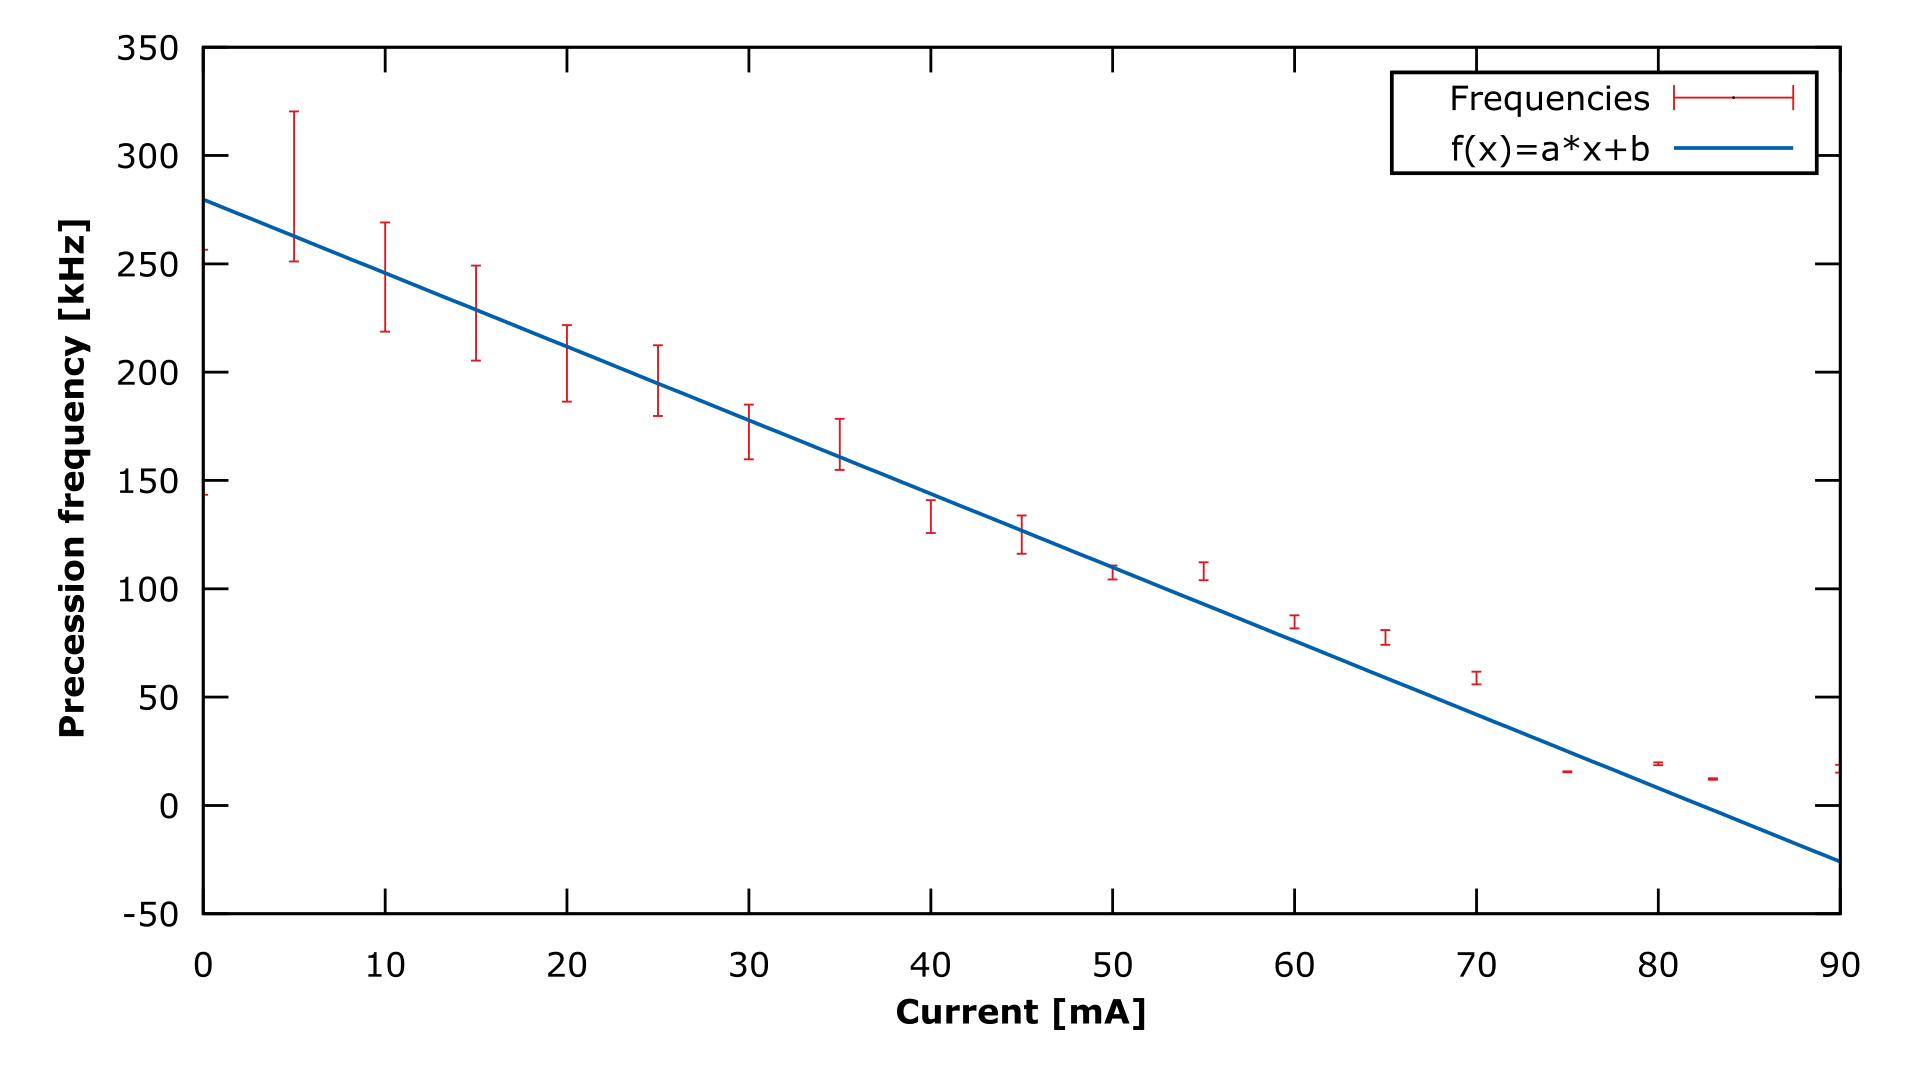
\includegraphics[width=1.0\linewidth]{graphics/freqlinfit}
\caption[Linear fit on precession frequencies]{The precession frequencies and the according linear fit. The x-axis cut can be calculated from the fit parameters and represents the current in coil 4 for which the vertical magnetic field is fully compensated.}
\label{fig:freqlinfit}
\end{figure}

\newpage
\section{Relaxation measurements - Dehmelt method}
\subsection{Set-up and procedure}
\begin{figure}
\centering
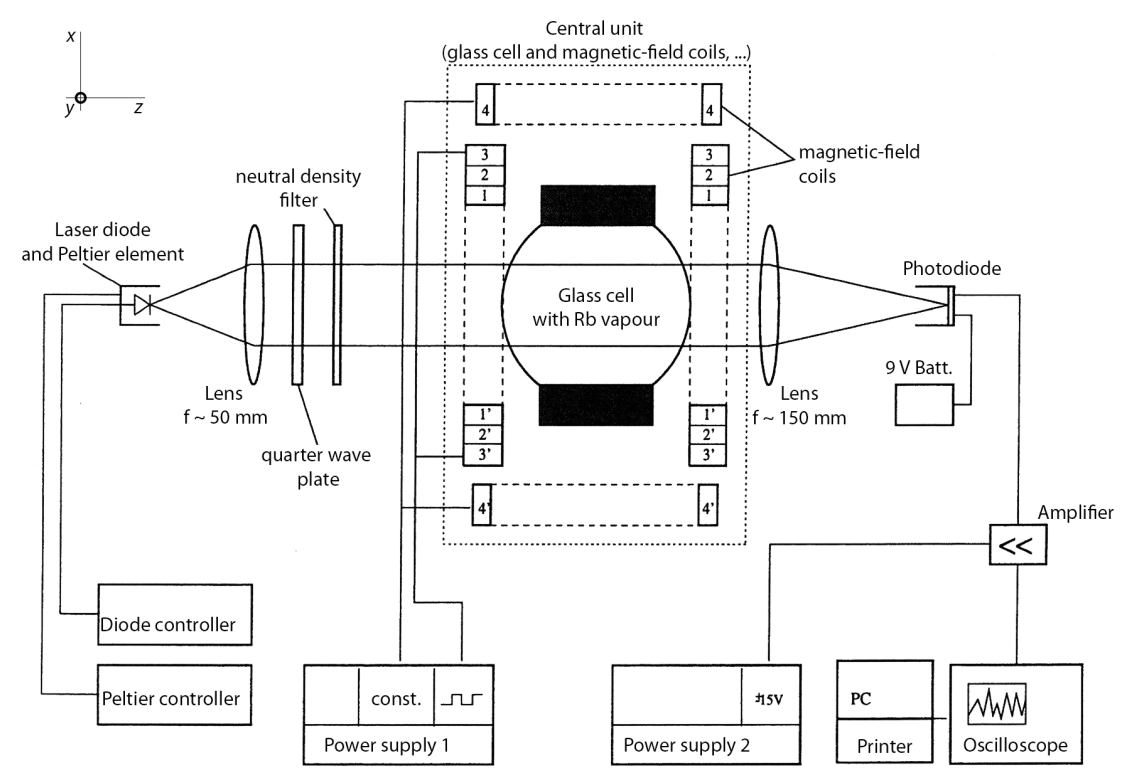
\includegraphics[width=1.0\linewidth]{graphics/dehmeltsetup}
\caption[Set-up relaxation measurements - Dehmelt]{Set-up for the relaxation measurements with the Dehmelt method. A range of neutral fitler was used. \cite{anleitung}}
\label{fig:dehmeltsetup}
\end{figure}
If the $^{87}$Rb atom were in a pumped state, say $F=2$ and $m_F=2$ for example, and the magnetic field responsible for the Zeeman splitting is suddenly reversed, the system is then pumped into the state $F=2$, $m_F=-2$. The measured intensity, after dropping sharply upon reversing the field, increases exponentially until the system is fully pumped. The speed of this process depends both on the laser intensity and speed of relaxation. If one measures this process for various laser intensities, facilitated with neutral filter (see fig. \ref{fig:dehmeltsetup}), the relaxation time $T_R$ of the system can be extracted as it remains constant. For these measurements, the vertical magnetic field will be compensated by coil 4 while coil 3 induces the reversing magnetic field.

\subsection{Data Analysis}
All measurements were taken at $T=\unit{34.3}{\degree}$ and a laser current of $I_L=\unit{61.6}{mA}$.\\
As the actual intensity reduction capabilities of the filter were unknown, a calibration measurement of all filters that are later to be used was done. First, a measurement of the intensity without any filter $I_{NF}$ and one of the intensity signal with the laser turned off $I_0$ were taken. The relative intensity of the former is then set as 1, the one of the latter as 0. The relative intensities for the filter $I^{rel}_F$ are calculated from their absolute measured intensities $I_F$ as
\begin{equation}
I^{rel}_F=\frac{I_F-I_0}{I_{NF}-I_0}
\end{equation}
Table \ref{tb:relintensities} shows the results of these calculations. The errors were calculated through Gaussian error propagation.\\ 
When available, the classification of the filter was used as a name. However, the filter named \emph{triangle} and \emph{circle} did not have a classification written on them, but instead the aforementioned symbols. 

\begin{table}\centering
	\begin{tabular}{@{}lllllll@{}}
		\toprule
		&Filter name&$I_L$ [V]&$I_{rel}$ [\%]&$s_{I_{rel}}$ [\%]&$\tau$ [ms]&$s_\tau$ [ms]\\ 
		\midrule
		&No filter&1.40&100.0&0.8&0.437&0.002\\
		&Triangle&1.11&80.1&0.7&0.503&0.002\\
		&Circle&0.68&50.8&0.6&0.712&0.002\\
		&-0,37&0.55&42.0&0.5&0.859&0.002\\
		&D0,3&0.50&38.5&0.5&0.842&0.002\\
		&0,6&0.48&37.4&0.5&1.121&0.05\\
		&D0,6&0.41&32.2&0.5&0.995&0.005\\
		&D1,0&0.39&31.2&0.5&1.574&0.008\\
		&-0,8&0.17&15.8&0.6&1.602&0.007\\
		&-1,03&0.16&15.2&0.6&2.048&0.023\\
		&D1,3&0.07&8.8&0.6&1.975&0.024\\
		&No laser&-0.06&0.0&0.6&-&-\\
		\bottomrule
	\end{tabular}
	\caption[Relative intensities of the filters]{The relative intensities for the neutral filters. Measurements were only possible for filter until the one marked D1,3.}
	\label{tb:relintensities}
\end{table}

For these filters, measurements of the relaxation time were taken. One such example can be seen in figure \ref{fig:dehmletexample}. Equation \ref{eq:orientationexponential} suggests using an exponential fit to describe the data:
\begin{equation}
I(t)=I_{max}-\Delta I\cdot e^{-a\cdot(t-t_0)}
\end{equation}
where $I_{max}$ is the intensity in the pumped state, $\Delta I$ the amplitude of the change in intensity and $t_0$ is an offset on the time axis to adjust for the fact that the magnetic field was not inverted at $t=0$. The deciding parameter however is $a=1/\tau$, the inverse of the orientation time of the system. The respective values for $\tau$ are listed in table \ref{tb:relintensities}. The values for $a$ can now be plotted against the relative intensities of the filter they were measured with. The result can be seen in figure \ref{fig:inversetaufit}.
\begin{figure}
\centering
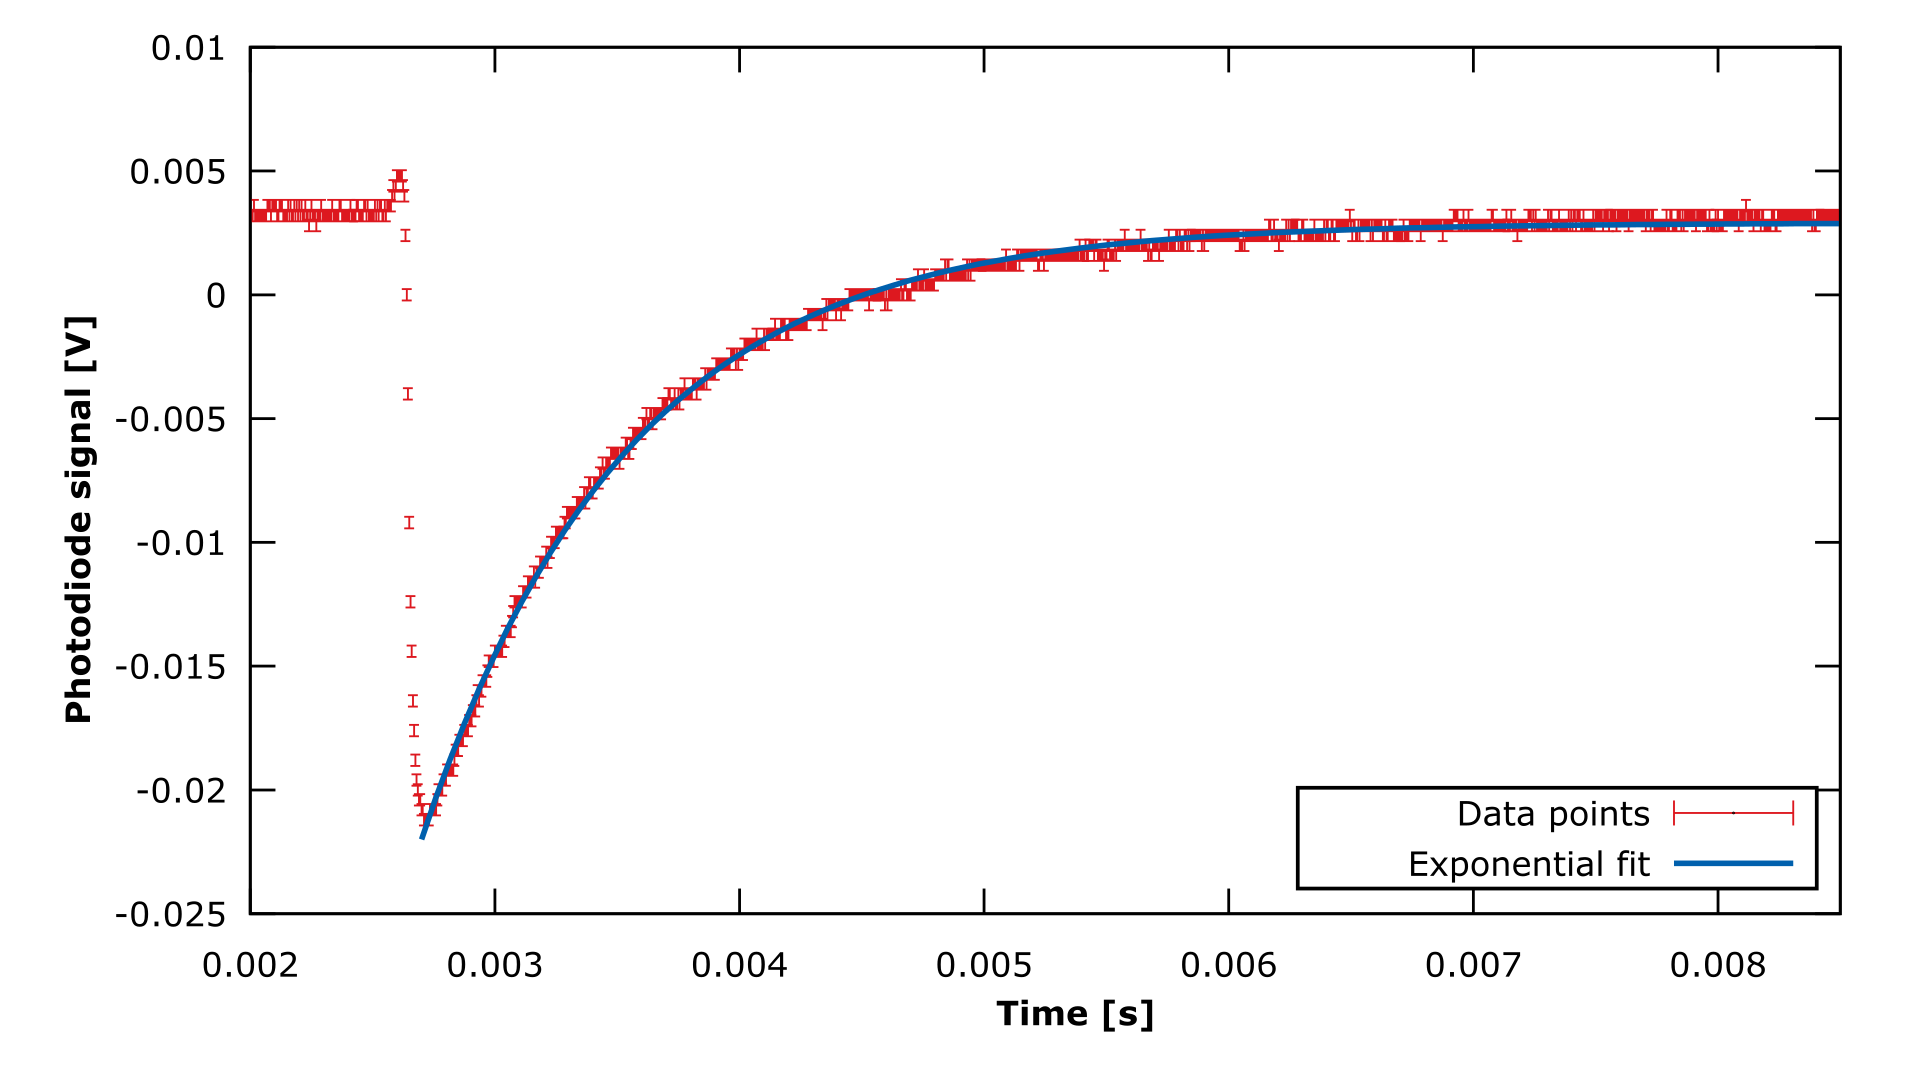
\includegraphics[width=1.0\linewidth]{graphics/dehmletexample}
\caption[Example of Dehmelt relaxation]{Relaxation data recorded with the neutral filter D0,3.}
\label{fig:dehmletexample}
\end{figure}
Equation \ref{eq:tauIrelation} and the fact the the pumping time is inversely proportional to the intensity, $T_P=\frac{1}{\alpha I}$, calls for a fit of the form
\begin{equation}
a(I_{rel})=\alpha I_{rel} + \frac{1}{T_R}
\end{equation}
The values a far more scattered than the uncertainties would suggest. This is expressed in a large $\chi^2\approx105$ as well as in a large error in the desired variable $T_R=\unit{(4.8\pm1.5)}{ms}$. Due to this large error, it includes the expected result of $T_R^{lit}=\unit{6.5}{ms}$ in its $2\sigma$ interval. One likely reason for the larger than expected fluctuation in inverse orientation times would be temperature fluctuations. These have a strong effect on the laser intensity.\\
In the theoretically calculated value, the spin-spin exchange was not taken into account and many calculations were simplified. This might also explain why the measured relaxation time is smaller than predicted.
\begin{figure}
\centering
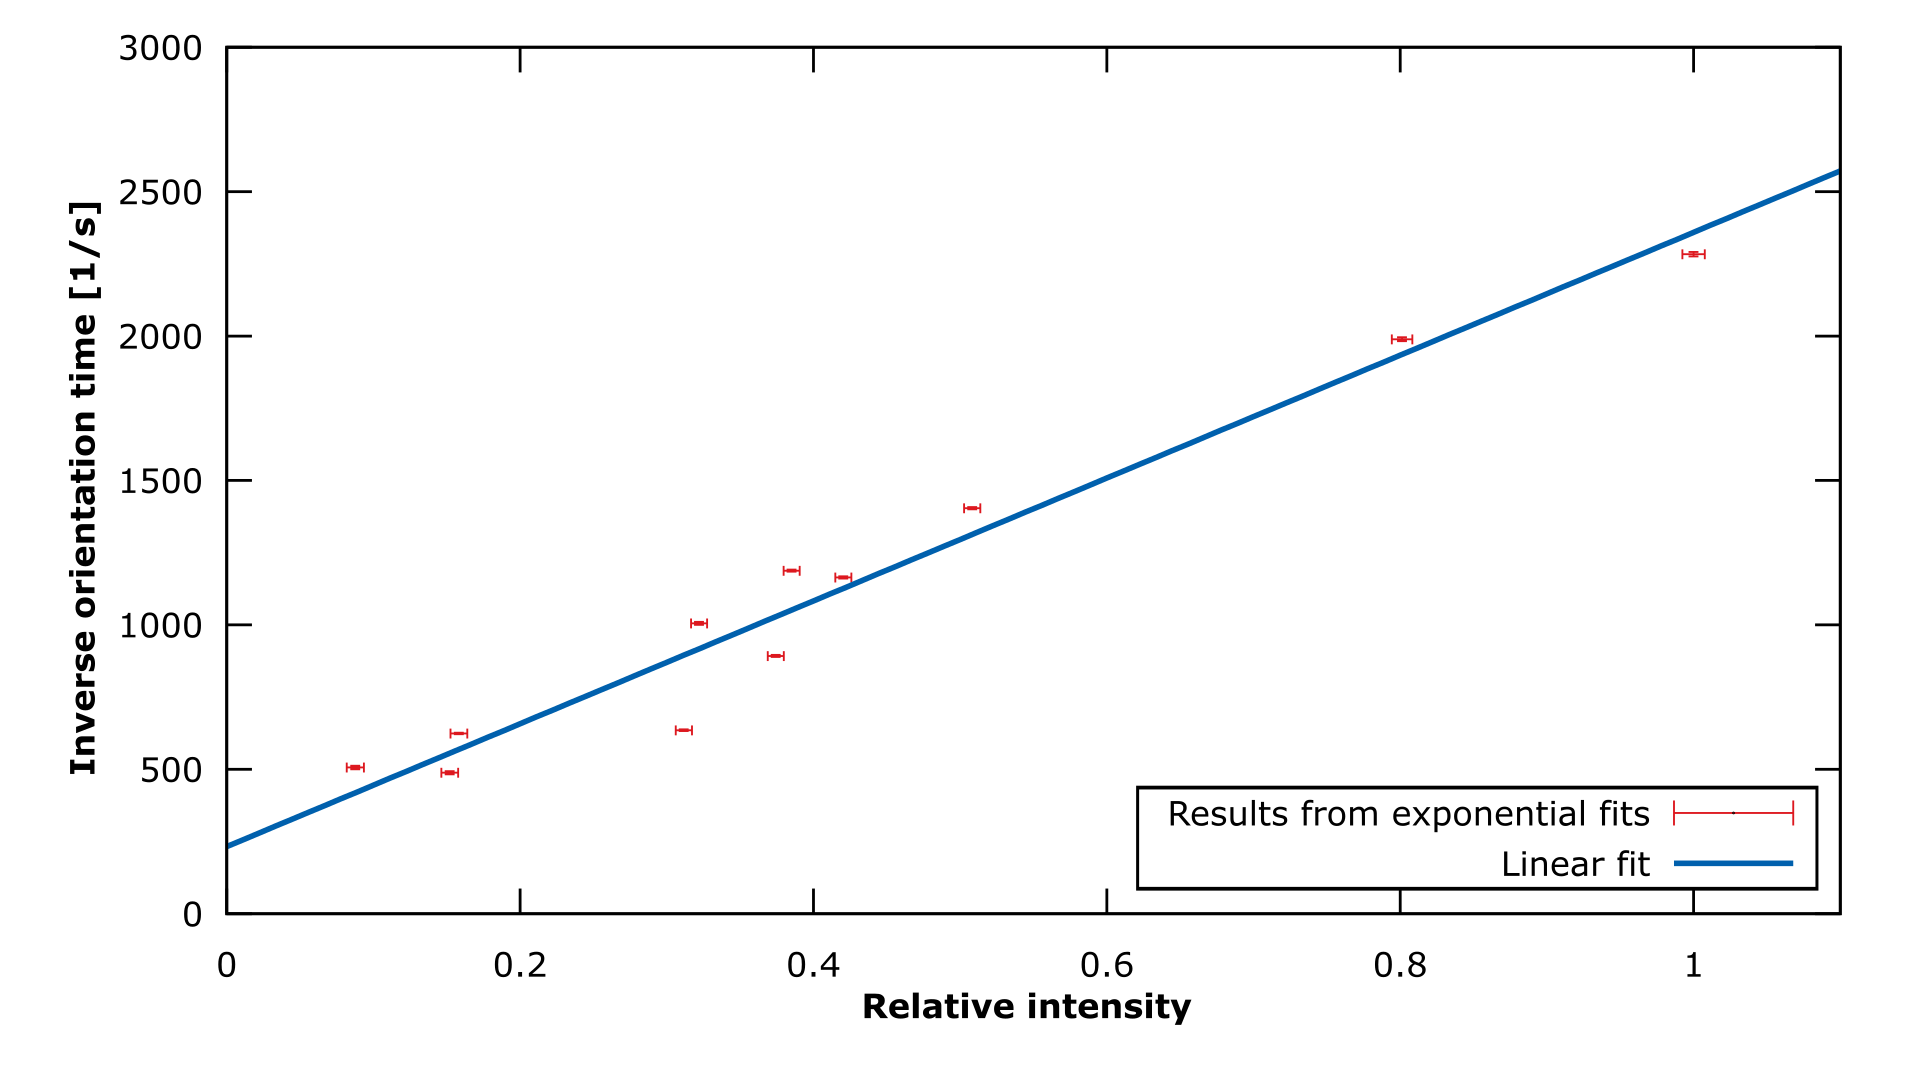
\includegraphics[width=1.0\linewidth]{graphics/inversetaufit}
\caption[Fit on the inverse orientation times]{The fit parameter $a$, which is the inverse orientation time, plotted for the respective relative intensity.}
\label{fig:inversetaufit}
\end{figure}


\newpage
\section{Relaxation measurements - Franzen method}
\subsection{Set-up and procedure}
\begin{figure}
\centering
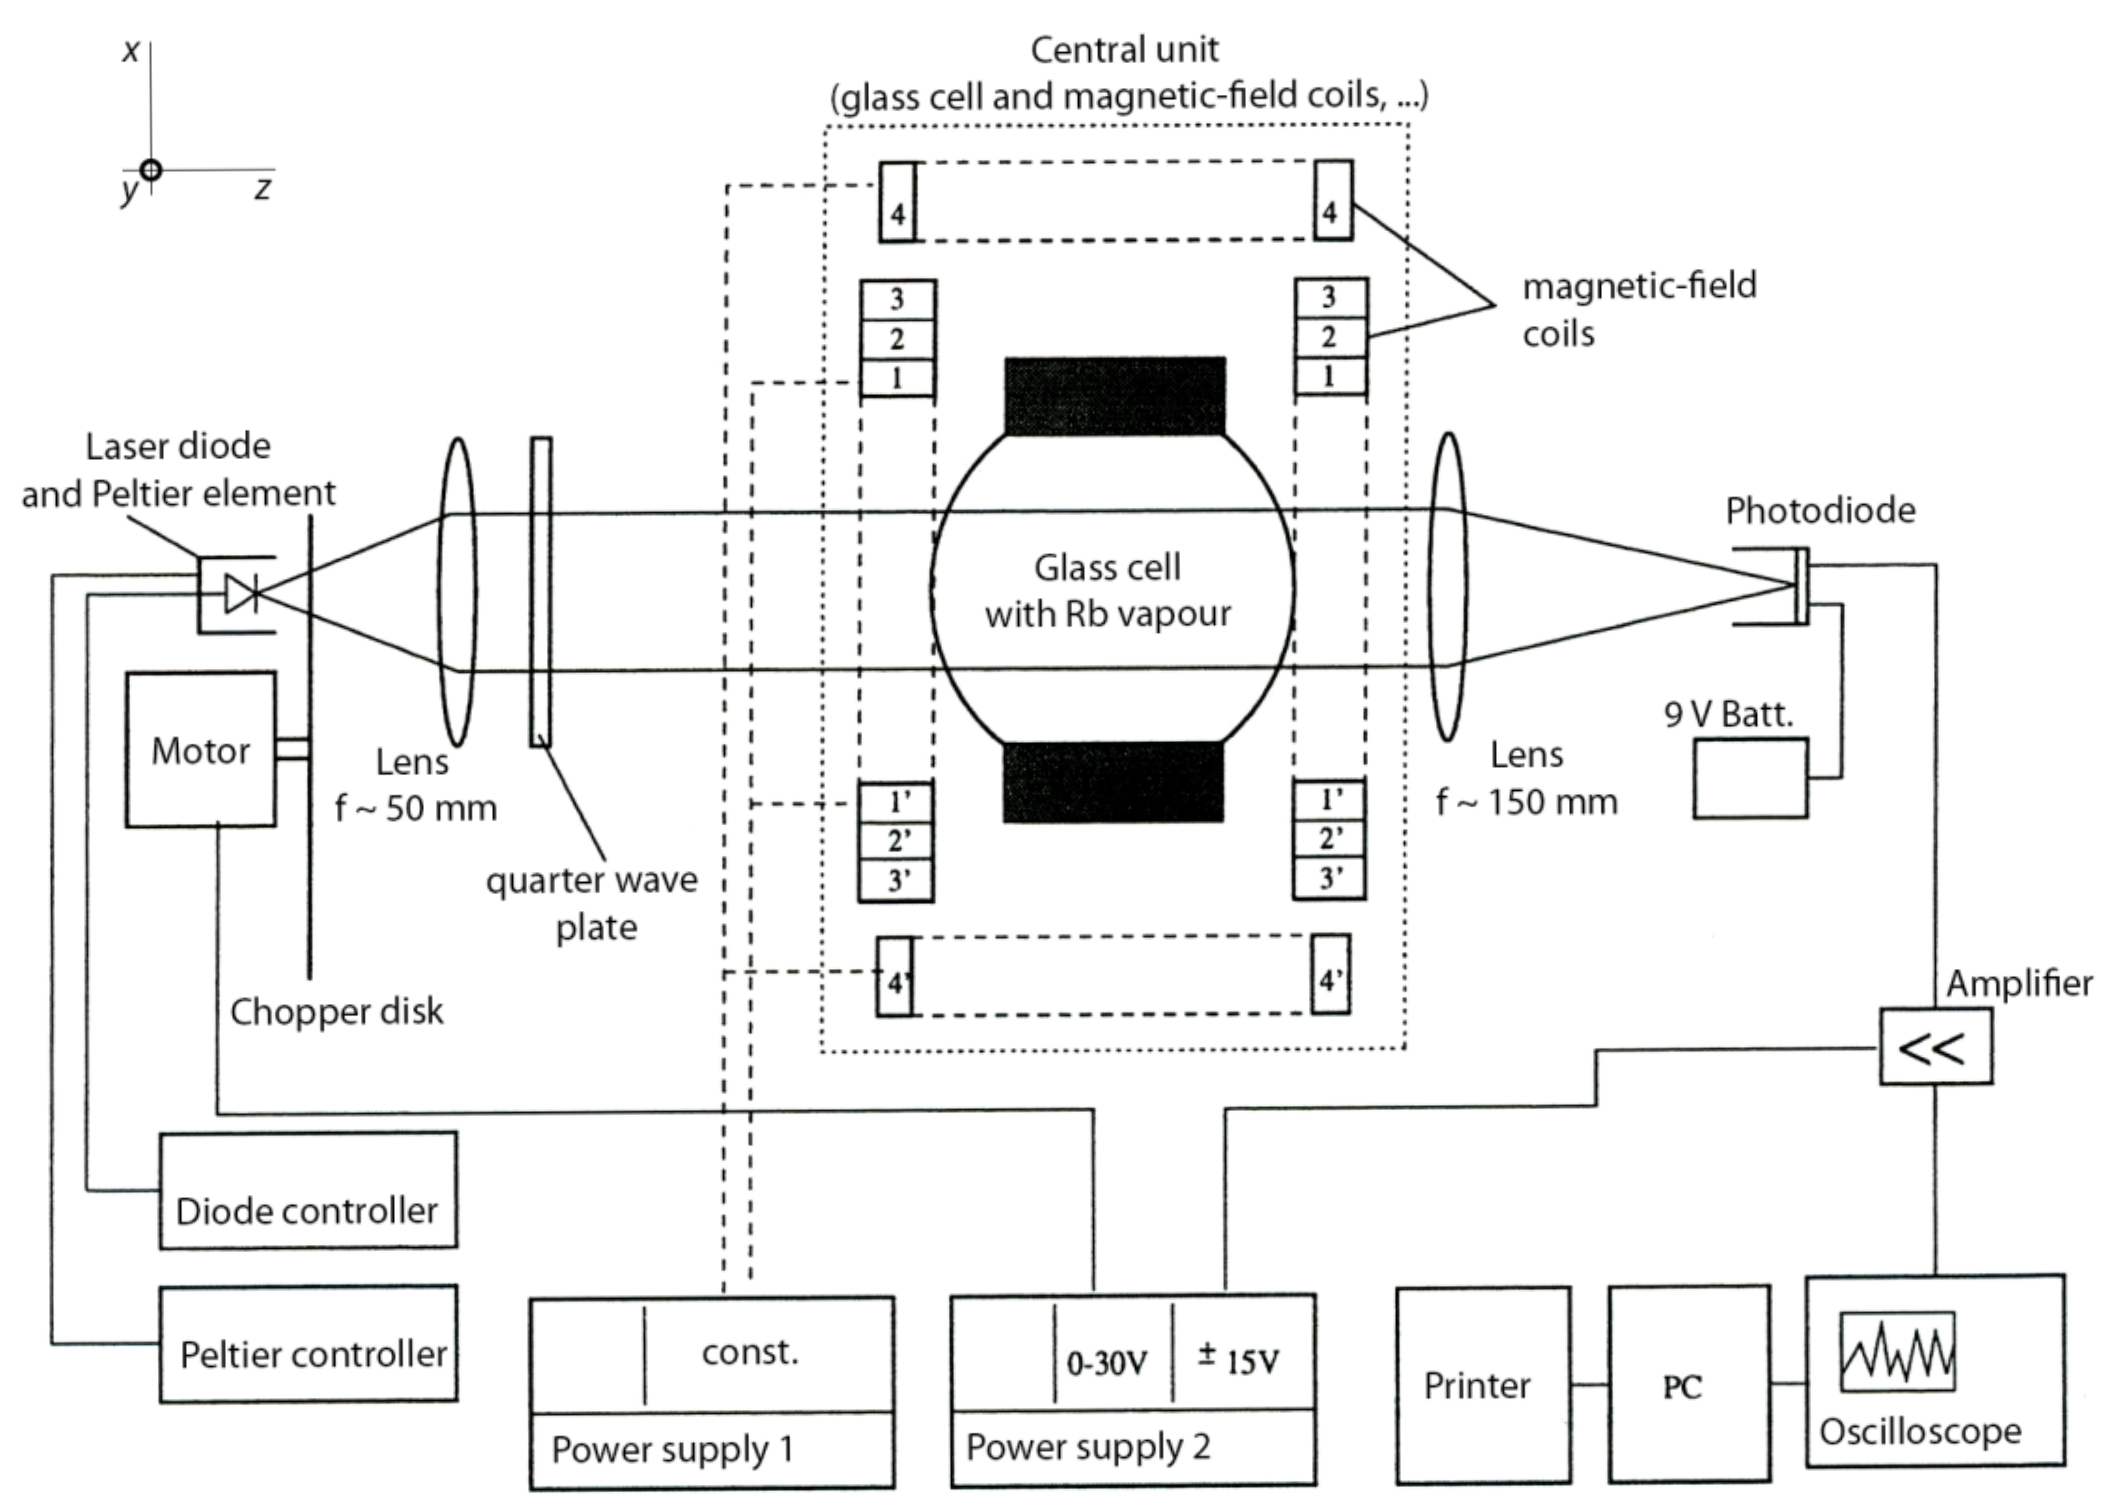
\includegraphics[width=1.0\linewidth]{graphics/franzensetup}
\caption[Set-up relaxation measurements - Franzen]{Set-up for the relaxation measurements with the Franzen method. The laser beam is periodicallz blocked with the chopper.\cite{anleitung}}
\label{fig:franzensetup}
\end{figure}
The Franzen method of determining the relaxation time relies on completely blocking and transmitting the laser. During the time when the laser is blocked ("darkness"), the system relaxes and, once the laser is transmitted again, causes exponentially dissipating absorption. The value from which the absorption reduces exponentially depends on the time for which the system was in darkness. The periodic blocking of the laser is facilitated by the chopper disk, which is placed as close to the laser as possible to make the cutting process faster. The laser current is set to maximize absorption signals.

\subsection{Data Analysis}
Measurements were taken at $T=\unit{34.3}{\degree}$ and $I_L=\unit{60.4}{mA}$. The vertical component of the earths' magnetic field remains compensated. For very low chopper voltages, the chopper signal was unstable and it was concluded that the motor does not operate steadily for such voltages. Measurements were then taken for motor voltages between $\unit{4}{V}$ and \unit{value}{unit}.
The results of one such measurement can be seen in figure 
For the fits, a Fermi function with a constant offset was used to approximate the intensity modulation by the chopper
\begin{equation}
I_{Ch}(t)=\frac{A}{1+e^{\frac{\mu-x}{\sigma}}}+U
\end{equation}
The relaxation, described by an exponential function, was made to start as soon as the Fermi function reaches 1\% intensity, which is true for $x>\mu-\sigma\log(99)$:
\begin{equation}
	I_R(t)=\begin{cases}
	0 &t\leq\mu-\sigma\log(99)\\
	B\cdot(1-e^{-\lambda(t-\mu)})&t\ge\mu-\sigma\log(99)
	\end{cases}
\end{equation}
\begin{figure}[htb]
	\centering
	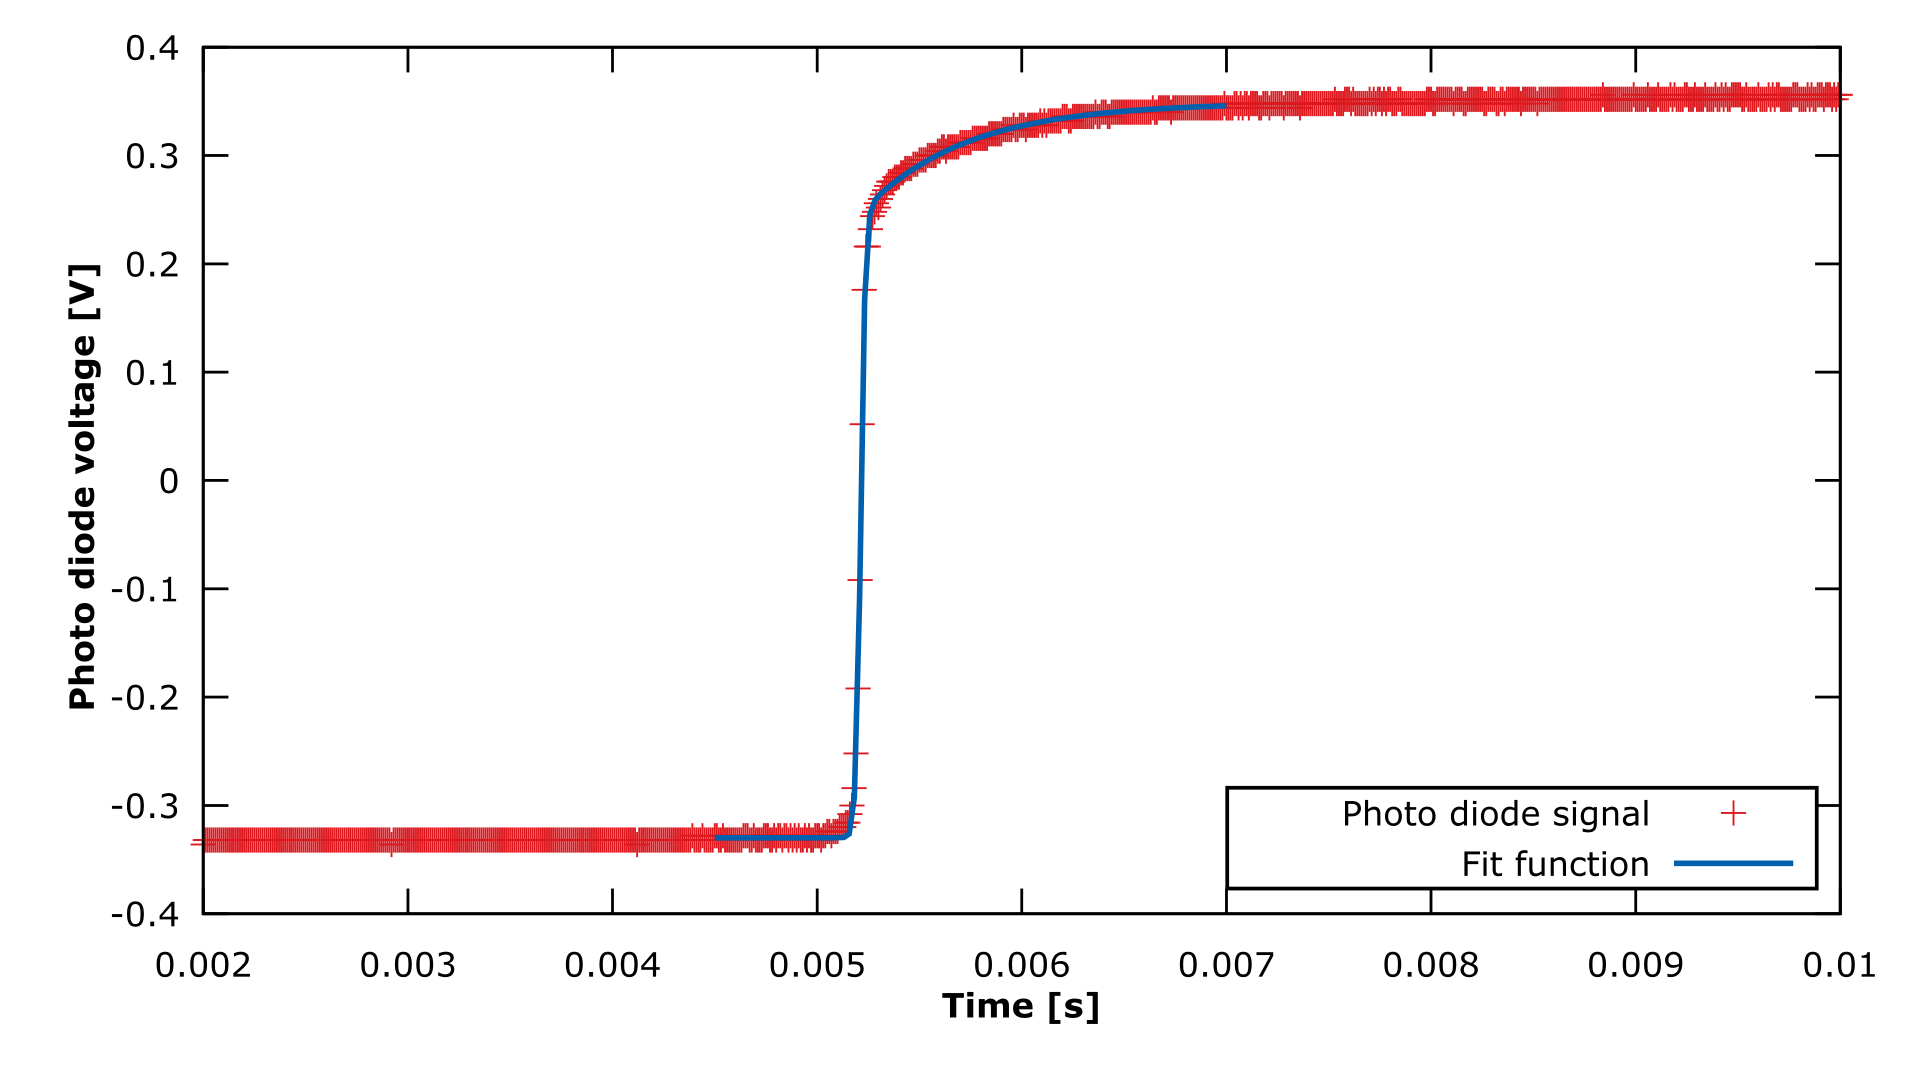
\includegraphics[width=1.0\linewidth]{graphics/franzenexample}
	\caption[Example of Franzen relaxation]{The relaxation measurement for a chopper voltage of \unit{4}{V} and the according fit.}
	\label{fig:franzenexample}
\end{figure}


These fits were very sensible to the starting parameters. The parameter $B$ is the absorption at $t=\mu-\sigma\log(99)$ and thus the sought after parameter. The dark times $t_d$ were taken from the data by hand and an uncertainty estimated each time. The parameter B for the different dark times can be seen in figure \ref{fig:Bparfit}. A fit of the form
\begin{equation}
B(t_d)=a+b\cdot(1-e^{-\frac{t_d}{T_R}})
\end{equation} 
where $a$ is an offset and $b$ is the amount of relaxation for large $t_d$. The data however is very linear and the fit thus converges only for very large $T_R$. The result for the relaxation time was
\begin{equation}
T_R=\unit{(50\pm24\cdot10^5)}{s}
\end{equation}

\begin{figure}
	\centering
	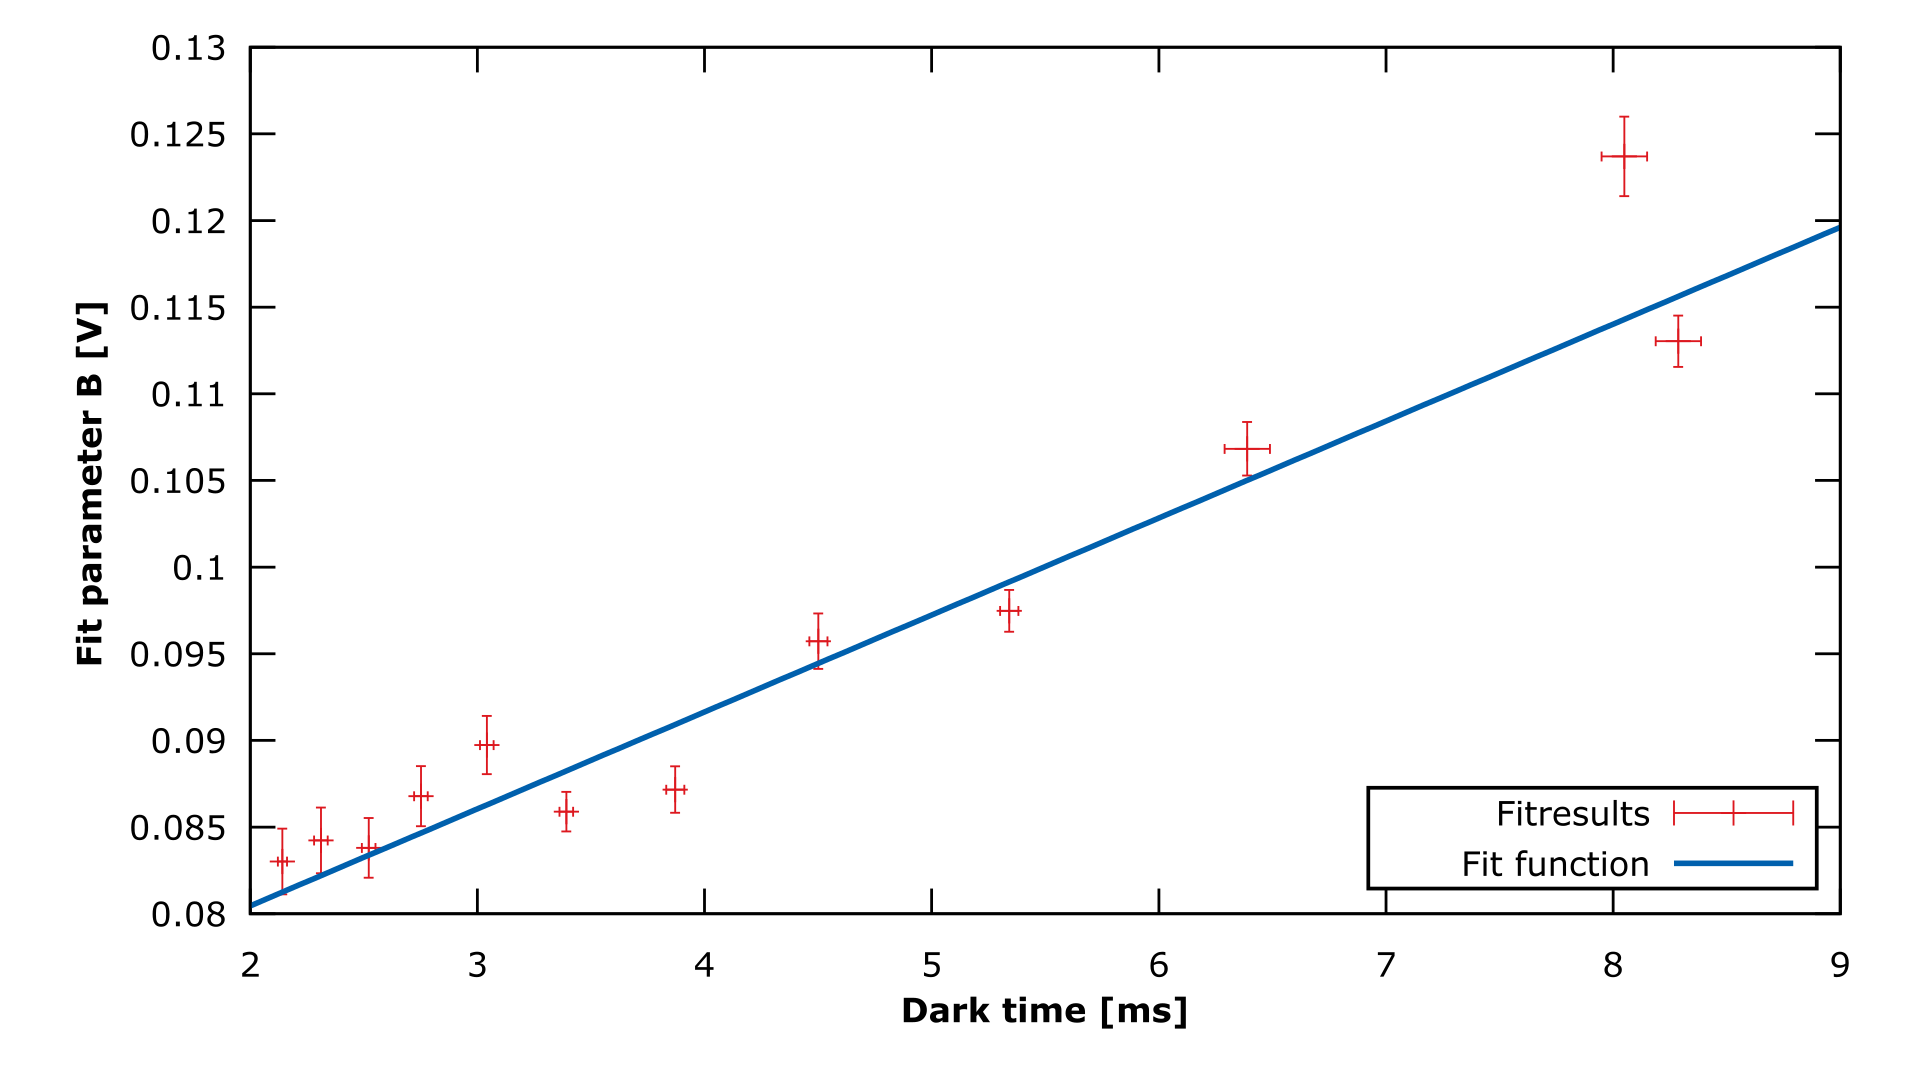
\includegraphics[width=1.0\linewidth]{graphics/Bparfit}
	\caption[Relaxation time fit Franzen]{The calculated fit parameters $B$ for the respective dark times.}
	\label{fig:Bparfit}
\end{figure}

Not only is the error astronomically large, the value is also several orders of magnitude away from the expected value of $T_R^{lit}=\unit{6.5}{ms}$. Longer dark times would likely have been needed for better measurements, but as mentioned before, the motor was not completely reliable for voltages below \unit{3}{V}. Figure \ref{fig:chopper1} shows the signal for \unit{1.5}{V}. The time that the edge of one opening in the chopper takes to fully pass by the laser is roughly \unit{0.5}{ms} and thus a significant time compared to the expected relaxation time of \unit{6.5}{ms}. Furthermore, the dark and light times seemed rather inconsistent, suggesting that the motor maybe does not operate at a constant speed. 



\begin{figure}
\centering
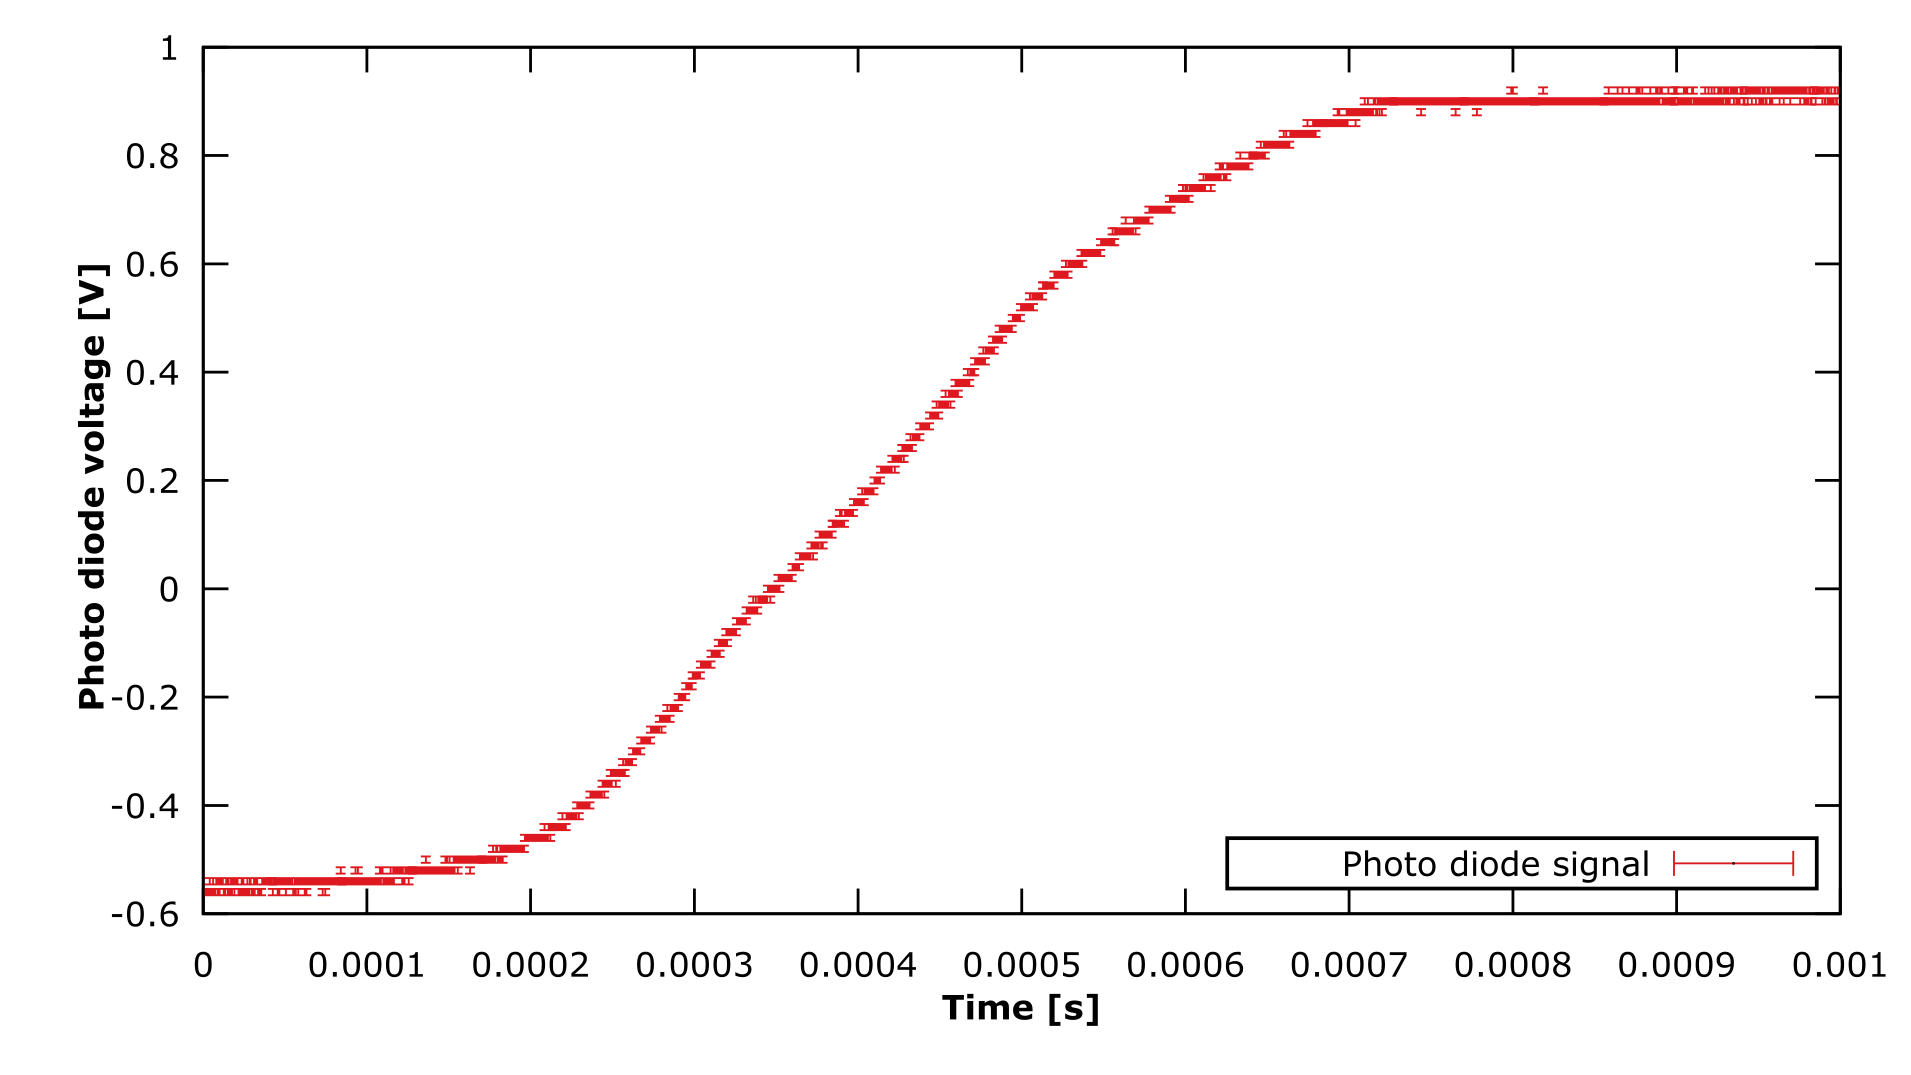
\includegraphics[width=1.0\linewidth]{graphics/chopper1,5V}
\caption[Chopper signal 1.5V]{The chopper signal for a supply voltage of \unit{1.5}{V}. The chopper takes roughly \unit{0.5}{ms} to fully pass by the laser. This is a significant time for the measurement period.}
\label{fig:chopper1}
\end{figure}





\newpage
\begin{thebibliography}{4}
	\bibitem{staatsex}
	Baur, Clemens. \emph{Einrichtung des Versuchs "Optisches Pumpen mit Laserdioden".}
	Zulassungsarbeit. Freiburg 1997
	\bibitem{anleitung}
	\emph{Instructions for the experiment "Optical Pumping".} Albert-Ludwig University Freiburg. Freiburg 02.2016
	\bibitem{happer}
	Happer, William. \emph{Optical pumping.}
	\ul{Reviews of Modern Physics} 44.2 (Apr. 1972): 170-238
	\bibitem{corney}
	Corney, A. \emph{Atomic and Laser Spectroscopy.}
	Oxford University Press, 1977
\end{thebibliography}
\appendix
\section{Appendix A: Measurement protocol}
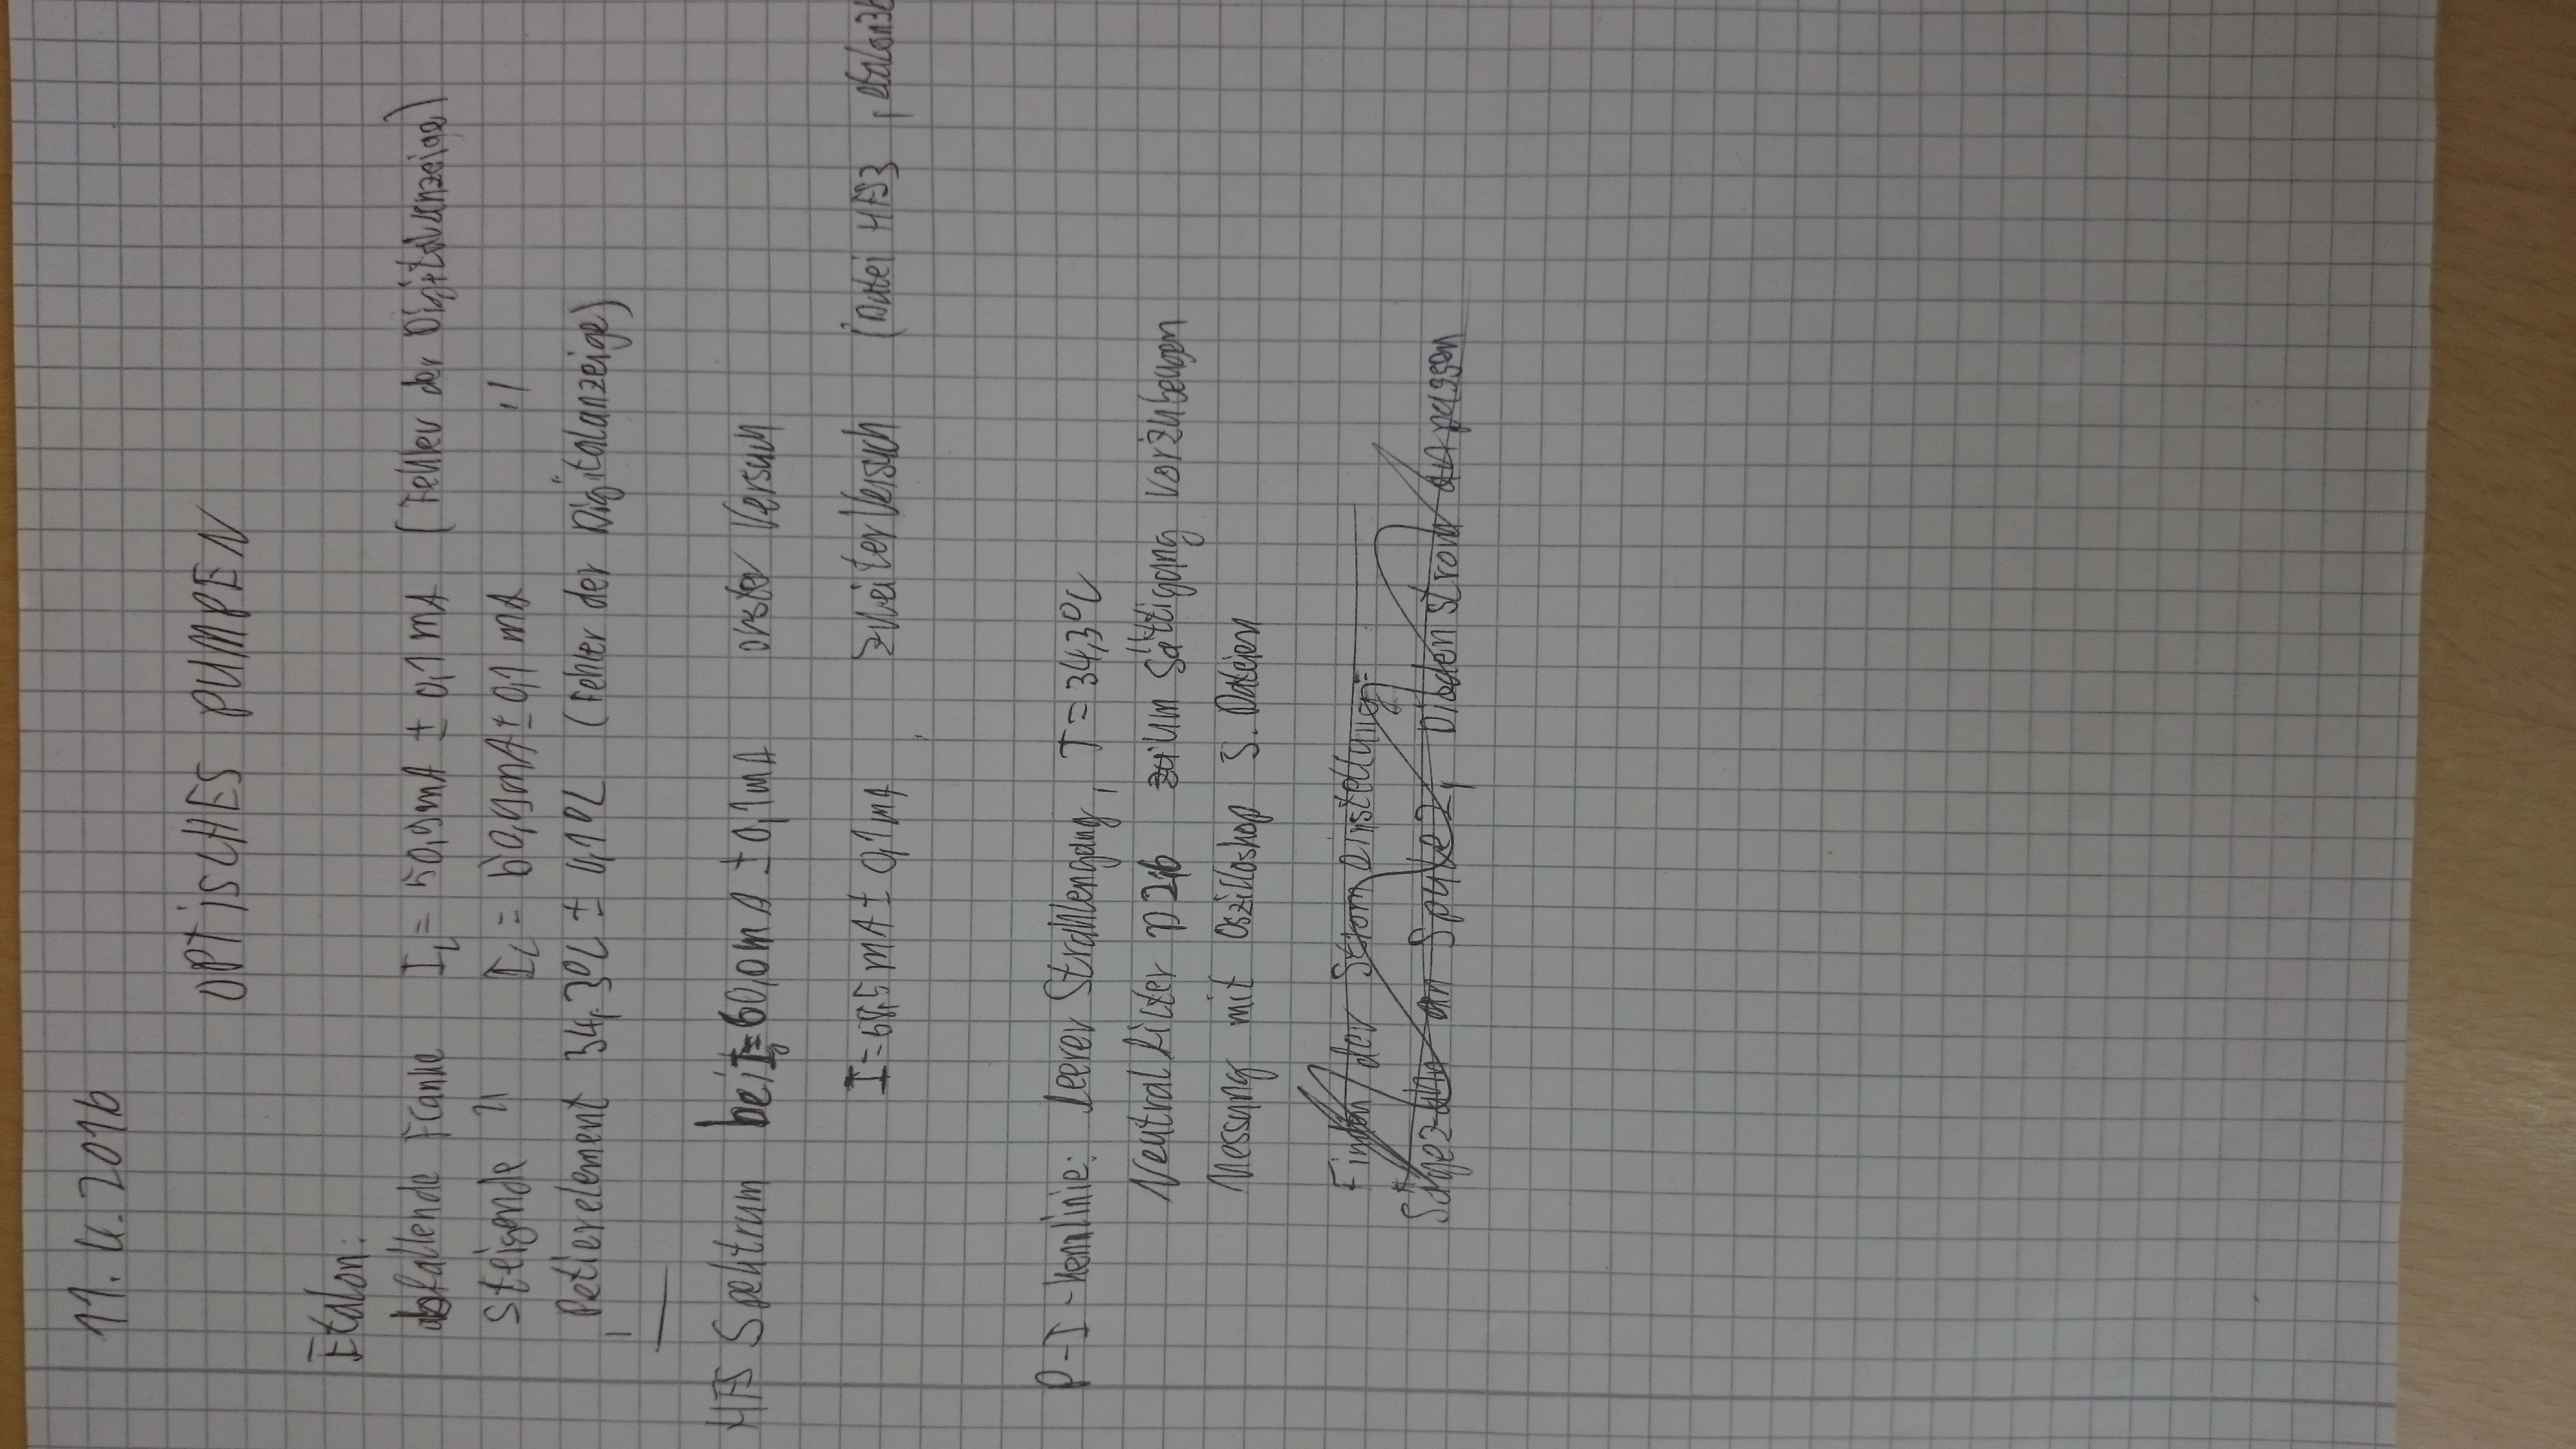
\includegraphics[angle=-90,width=1.0\linewidth]{graphics/DSC_0086}
\newpage
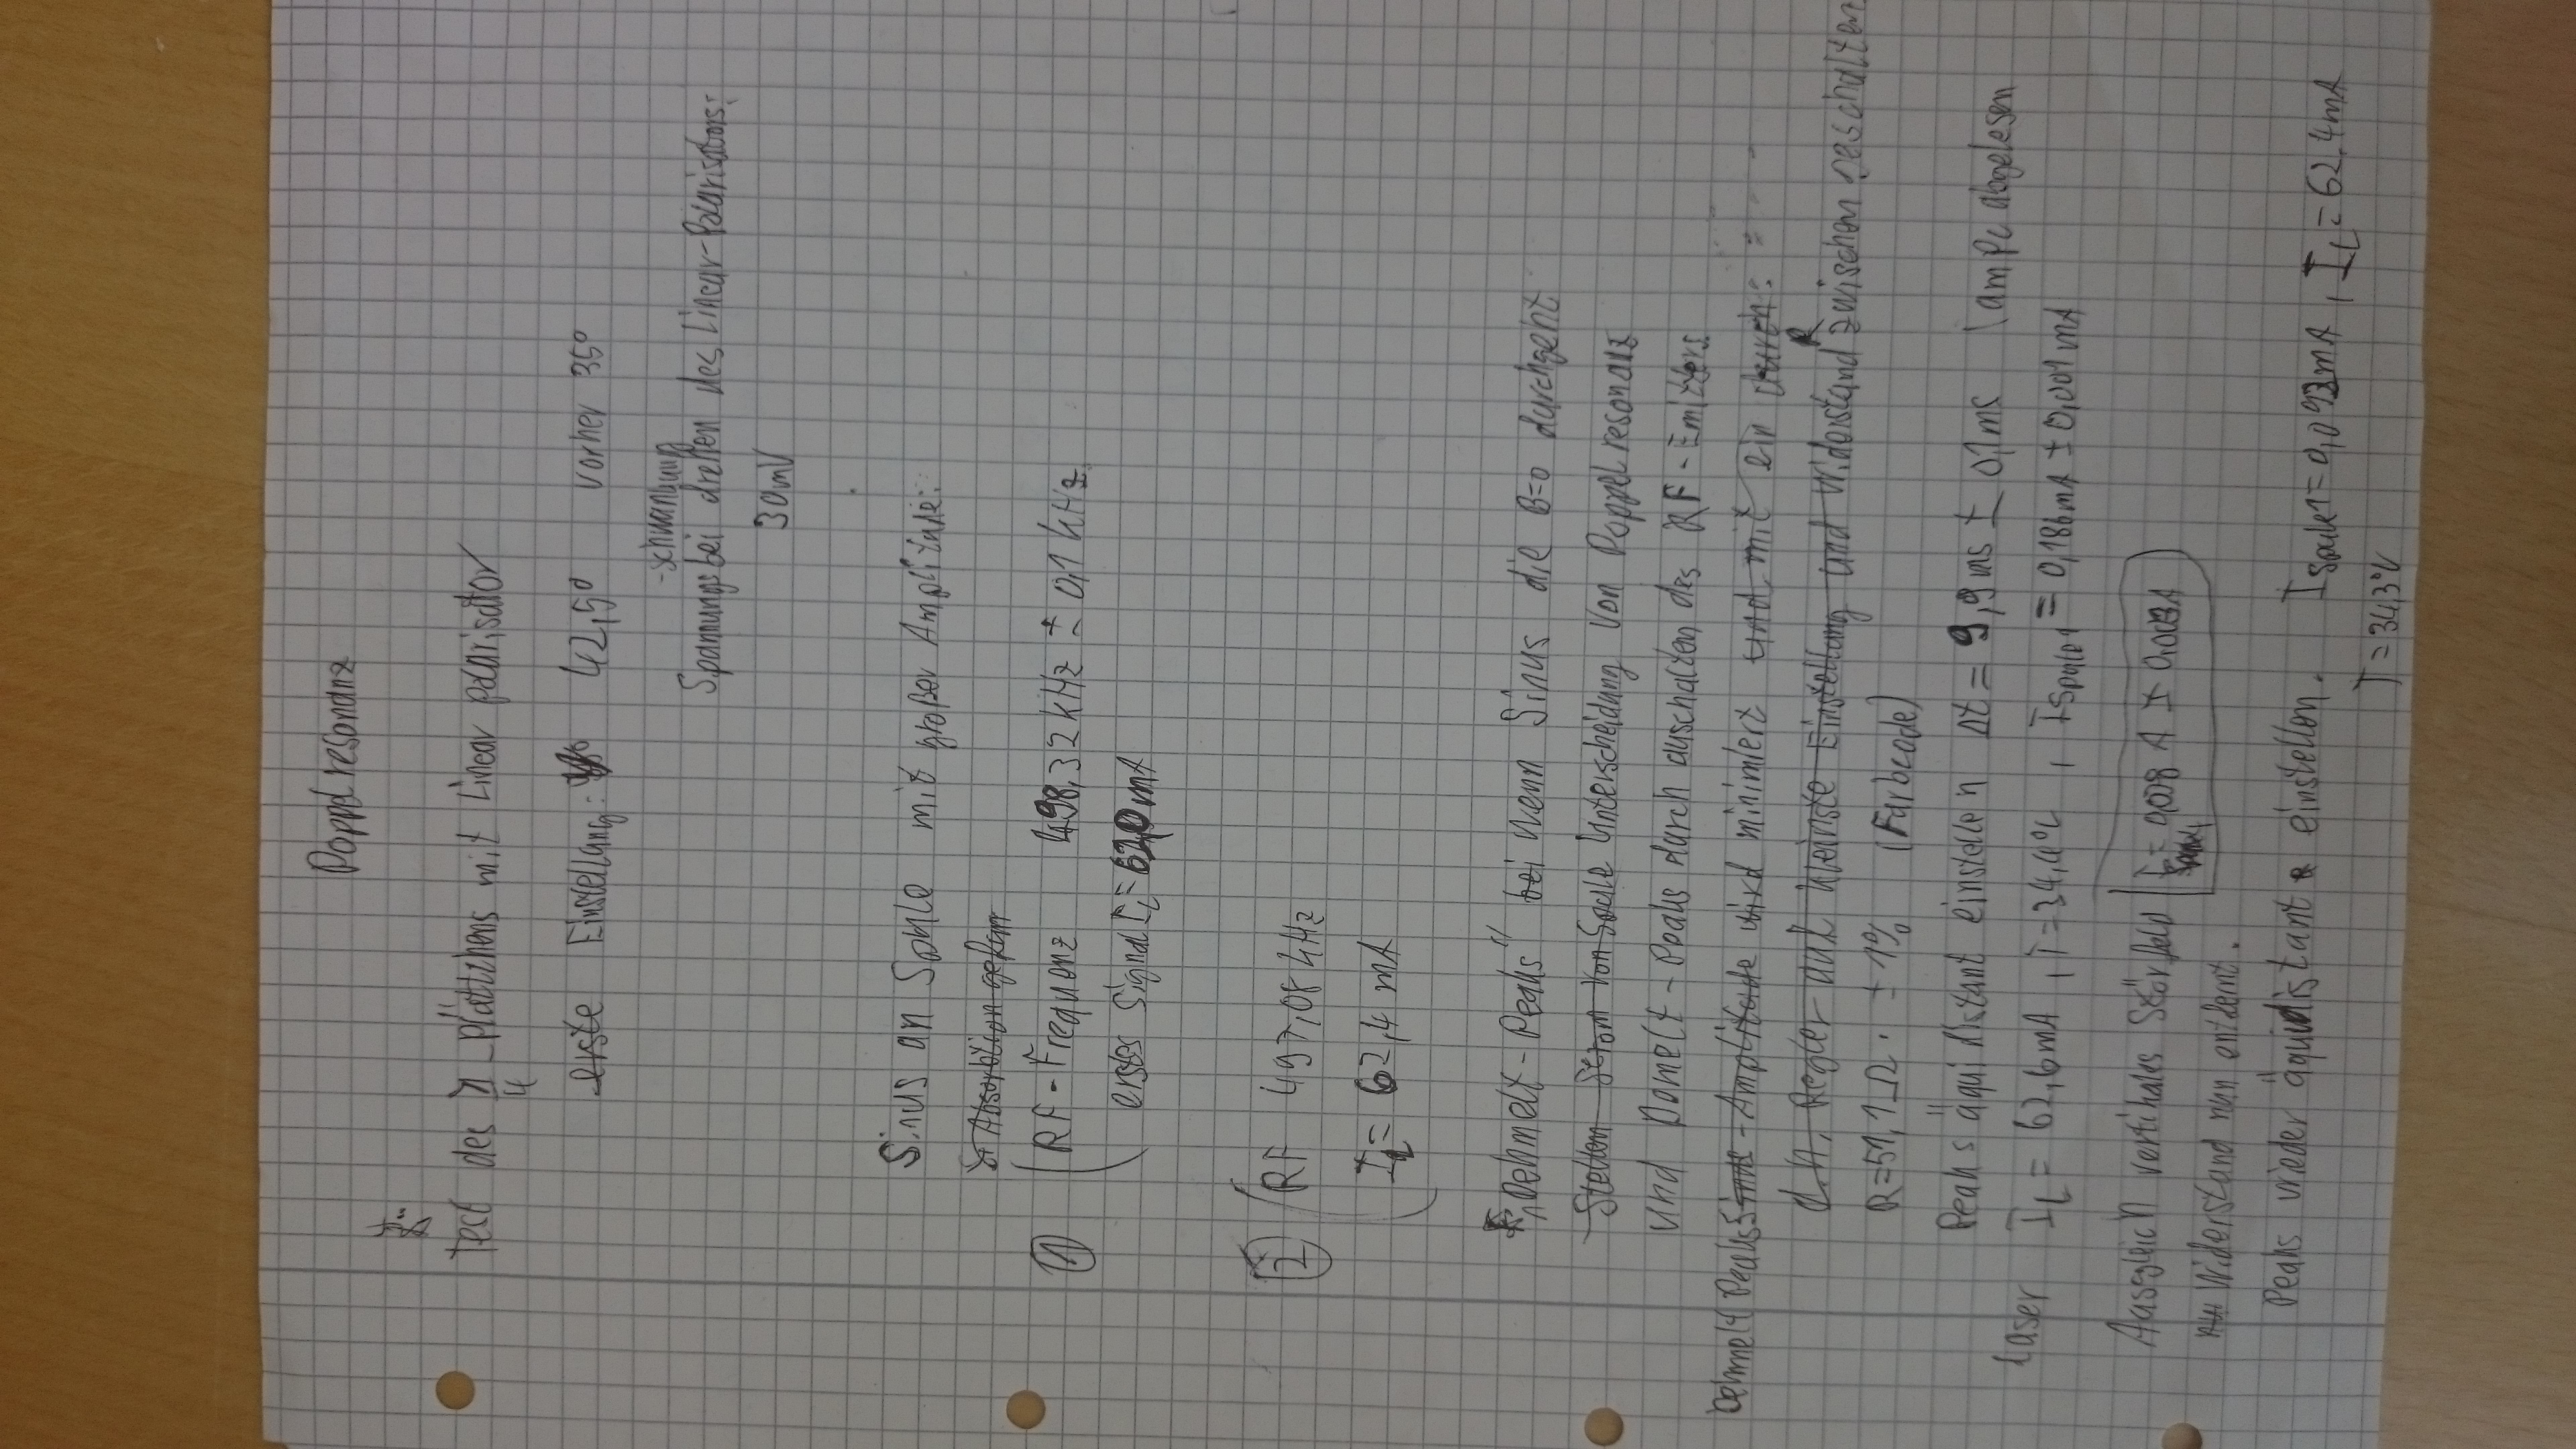
\includegraphics[angle=-90,width=1.0\linewidth]{graphics/DSC_0087}
\newpage
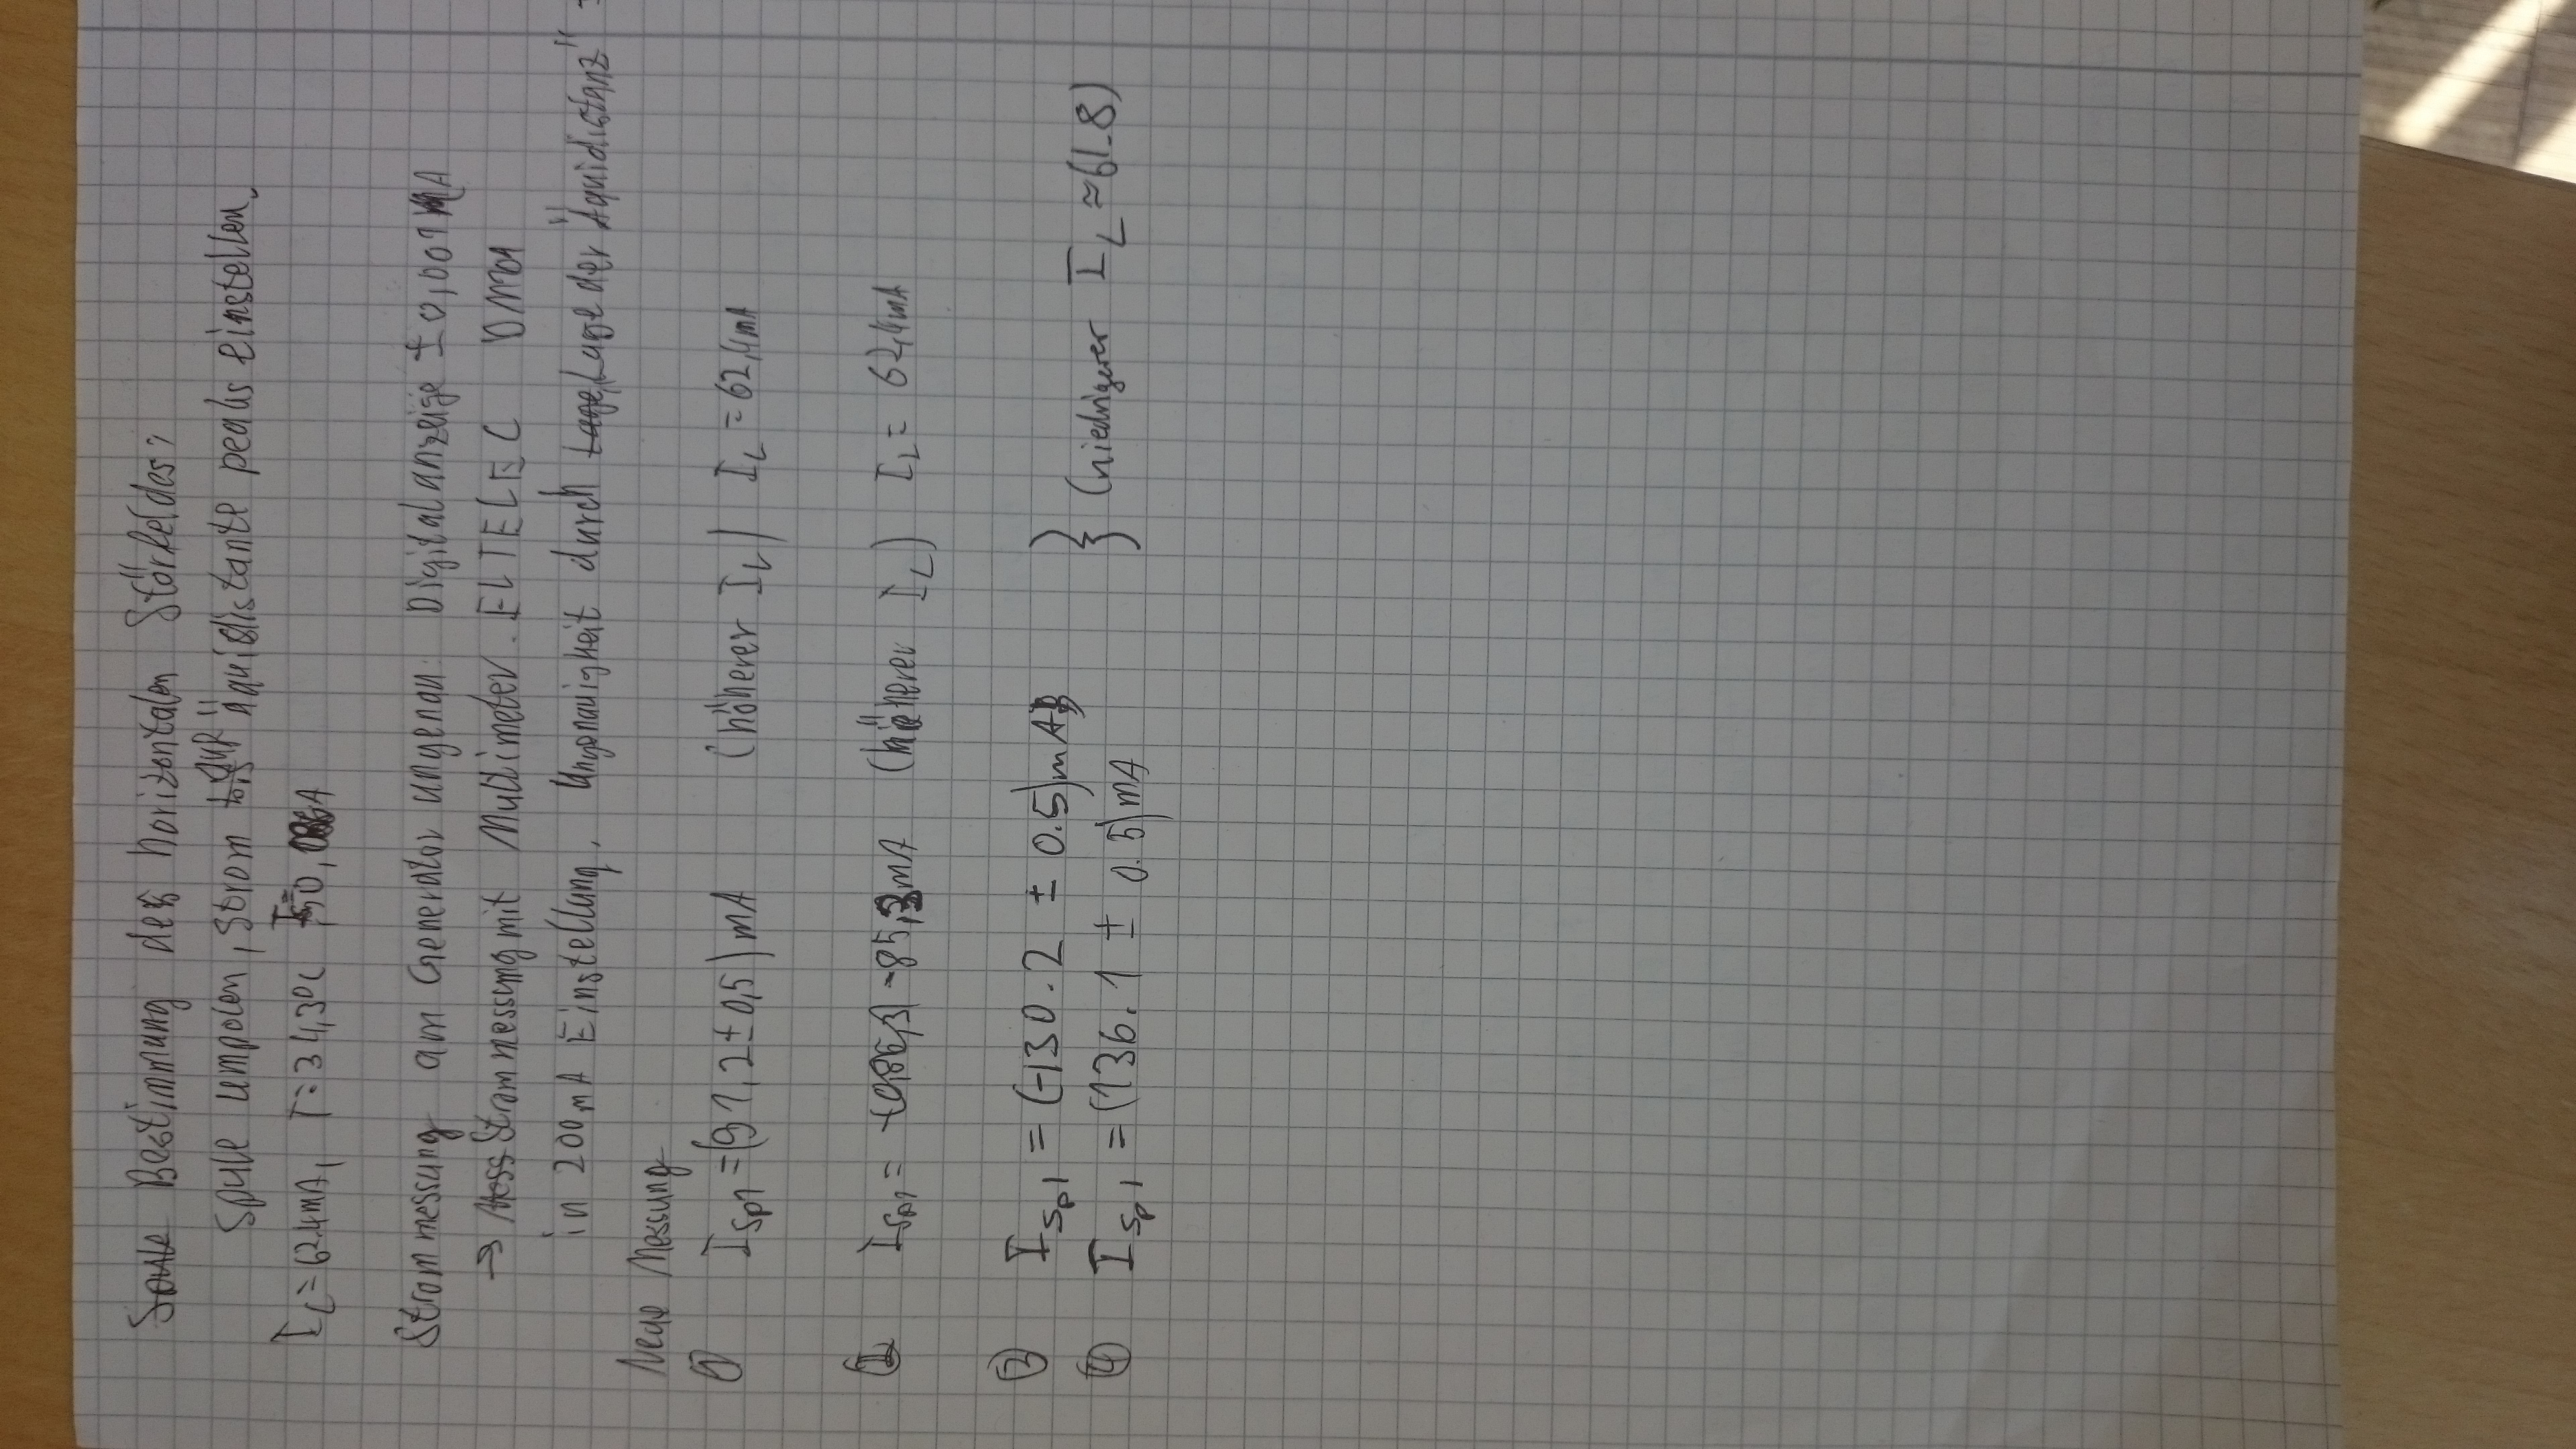
\includegraphics[angle=-90,width=1.0\linewidth]{graphics/DSC_0088}
\newpage
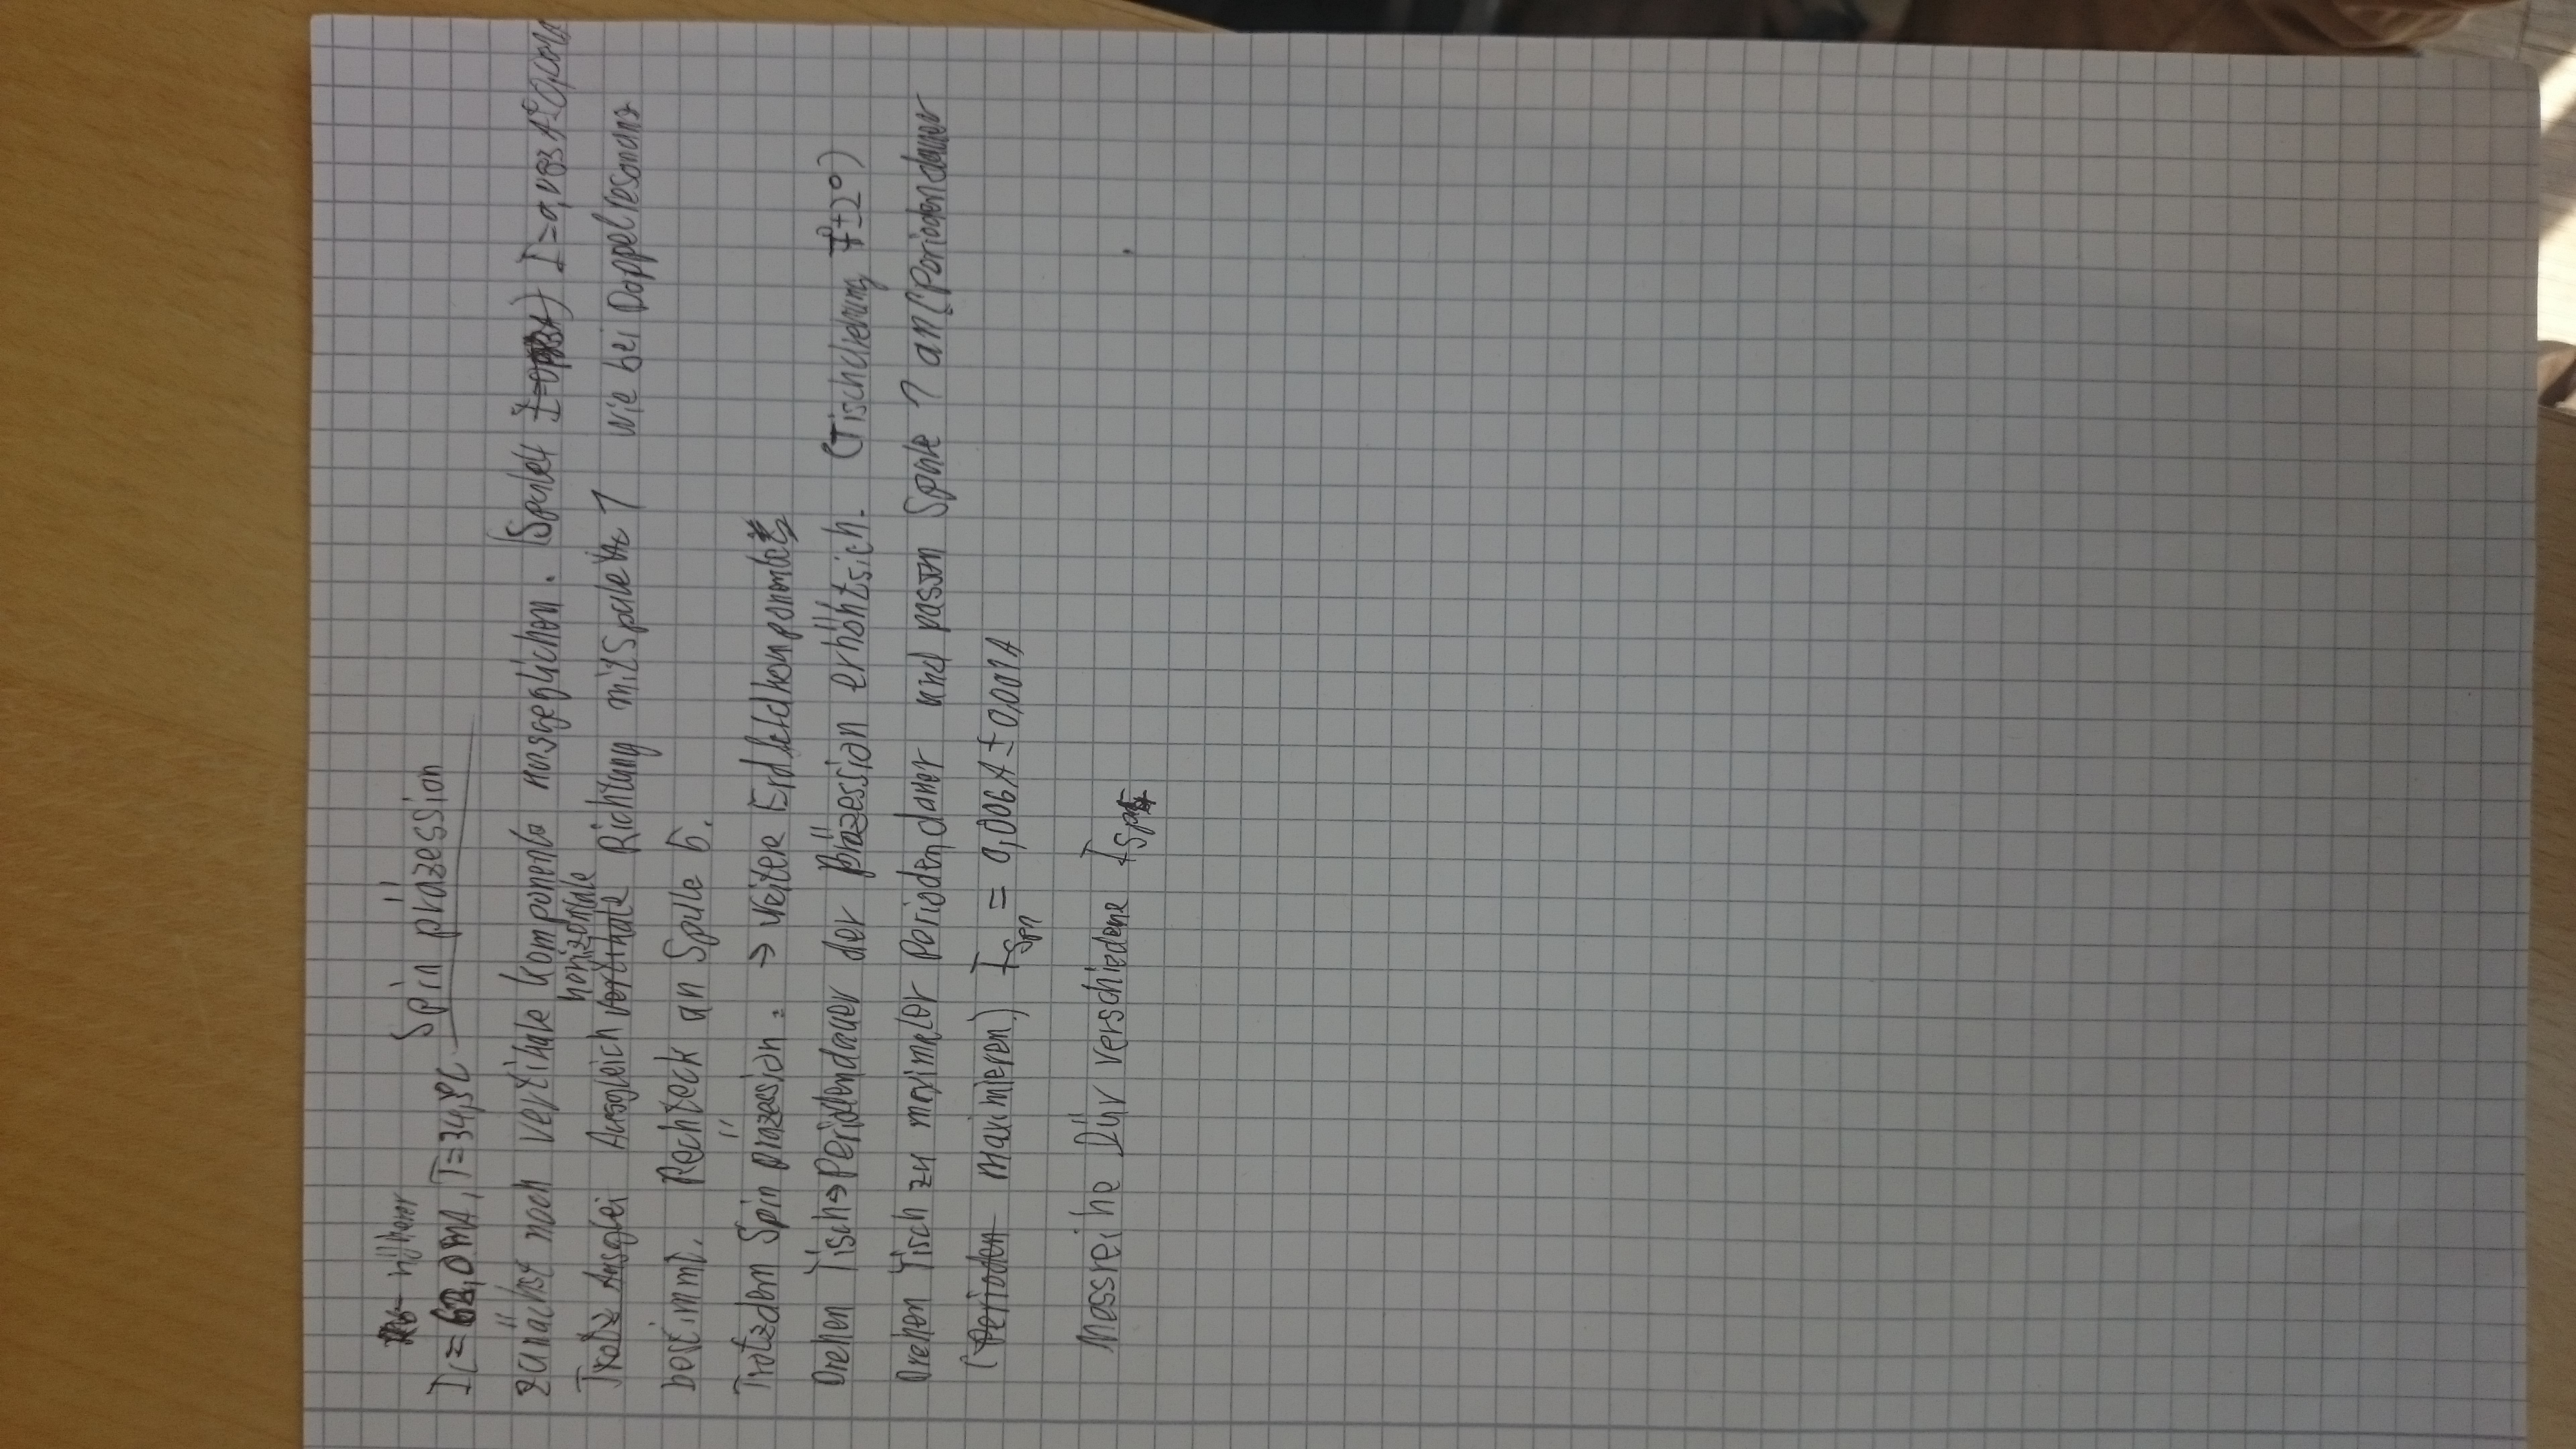
\includegraphics[angle=-90,width=1.0\linewidth]{graphics/DSC_0089}
\newpage
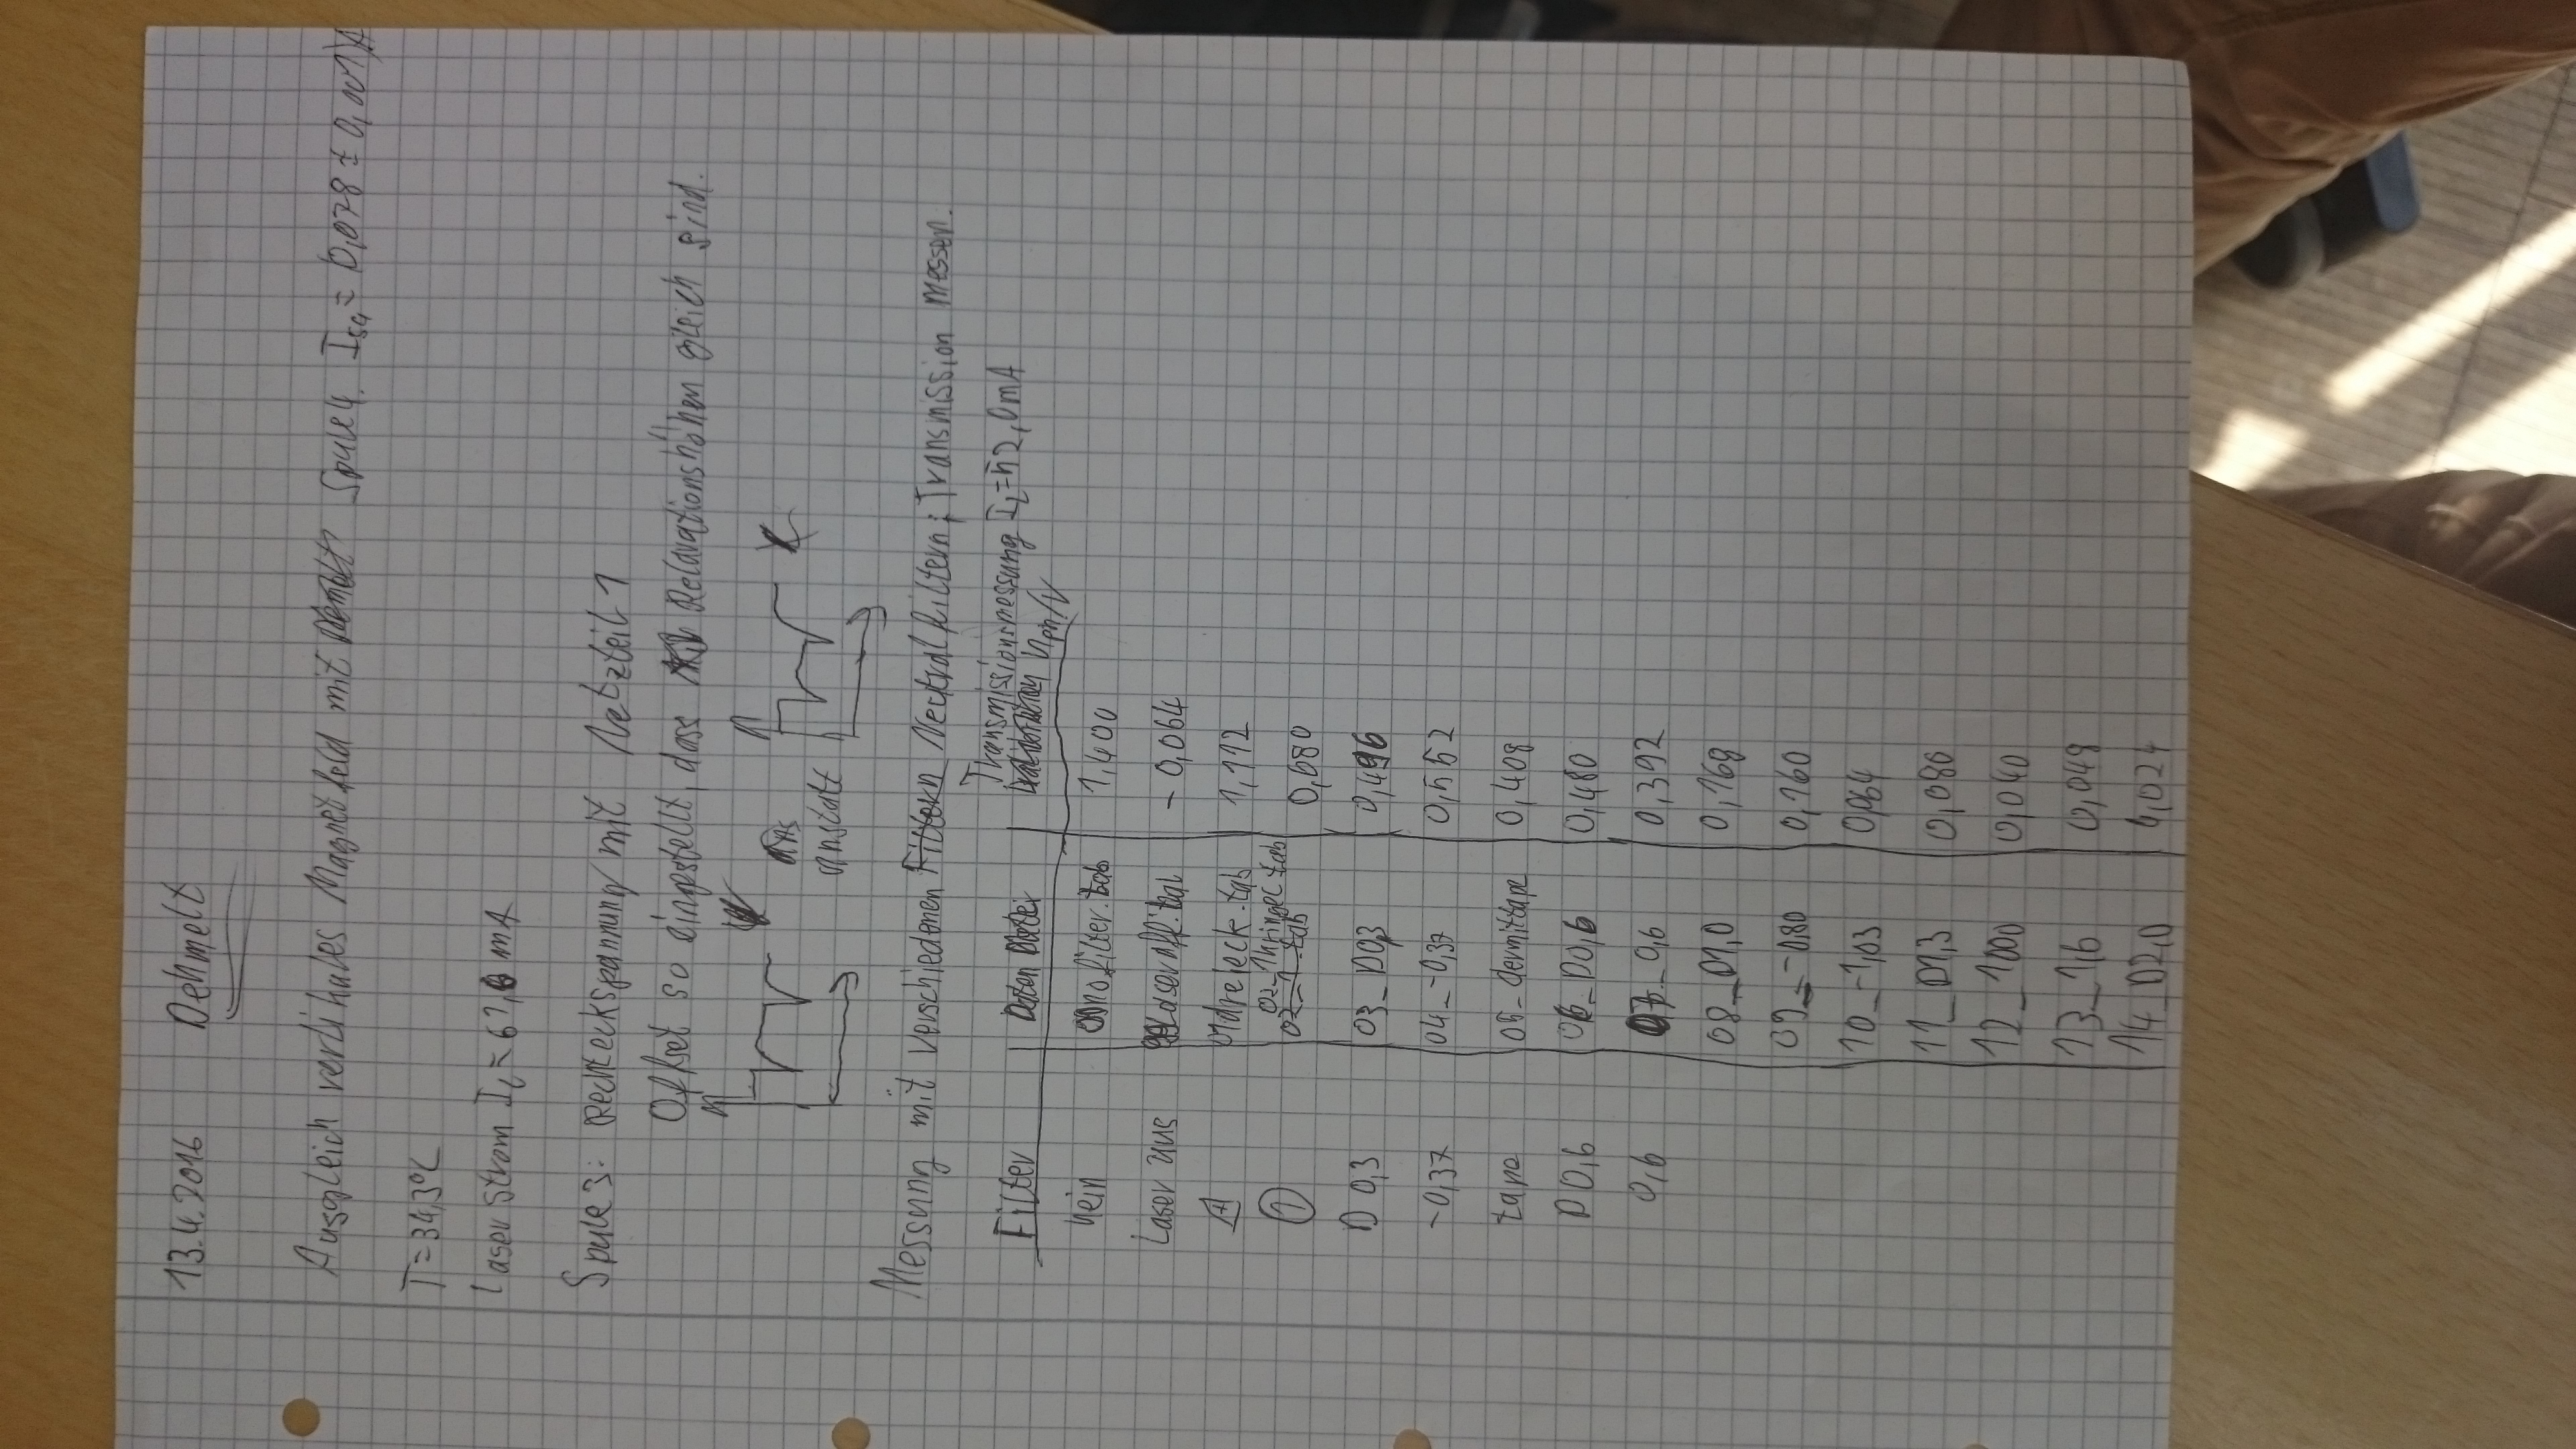
\includegraphics[angle=-90,width=1.0\linewidth]{graphics/DSC_0090}
\newpage
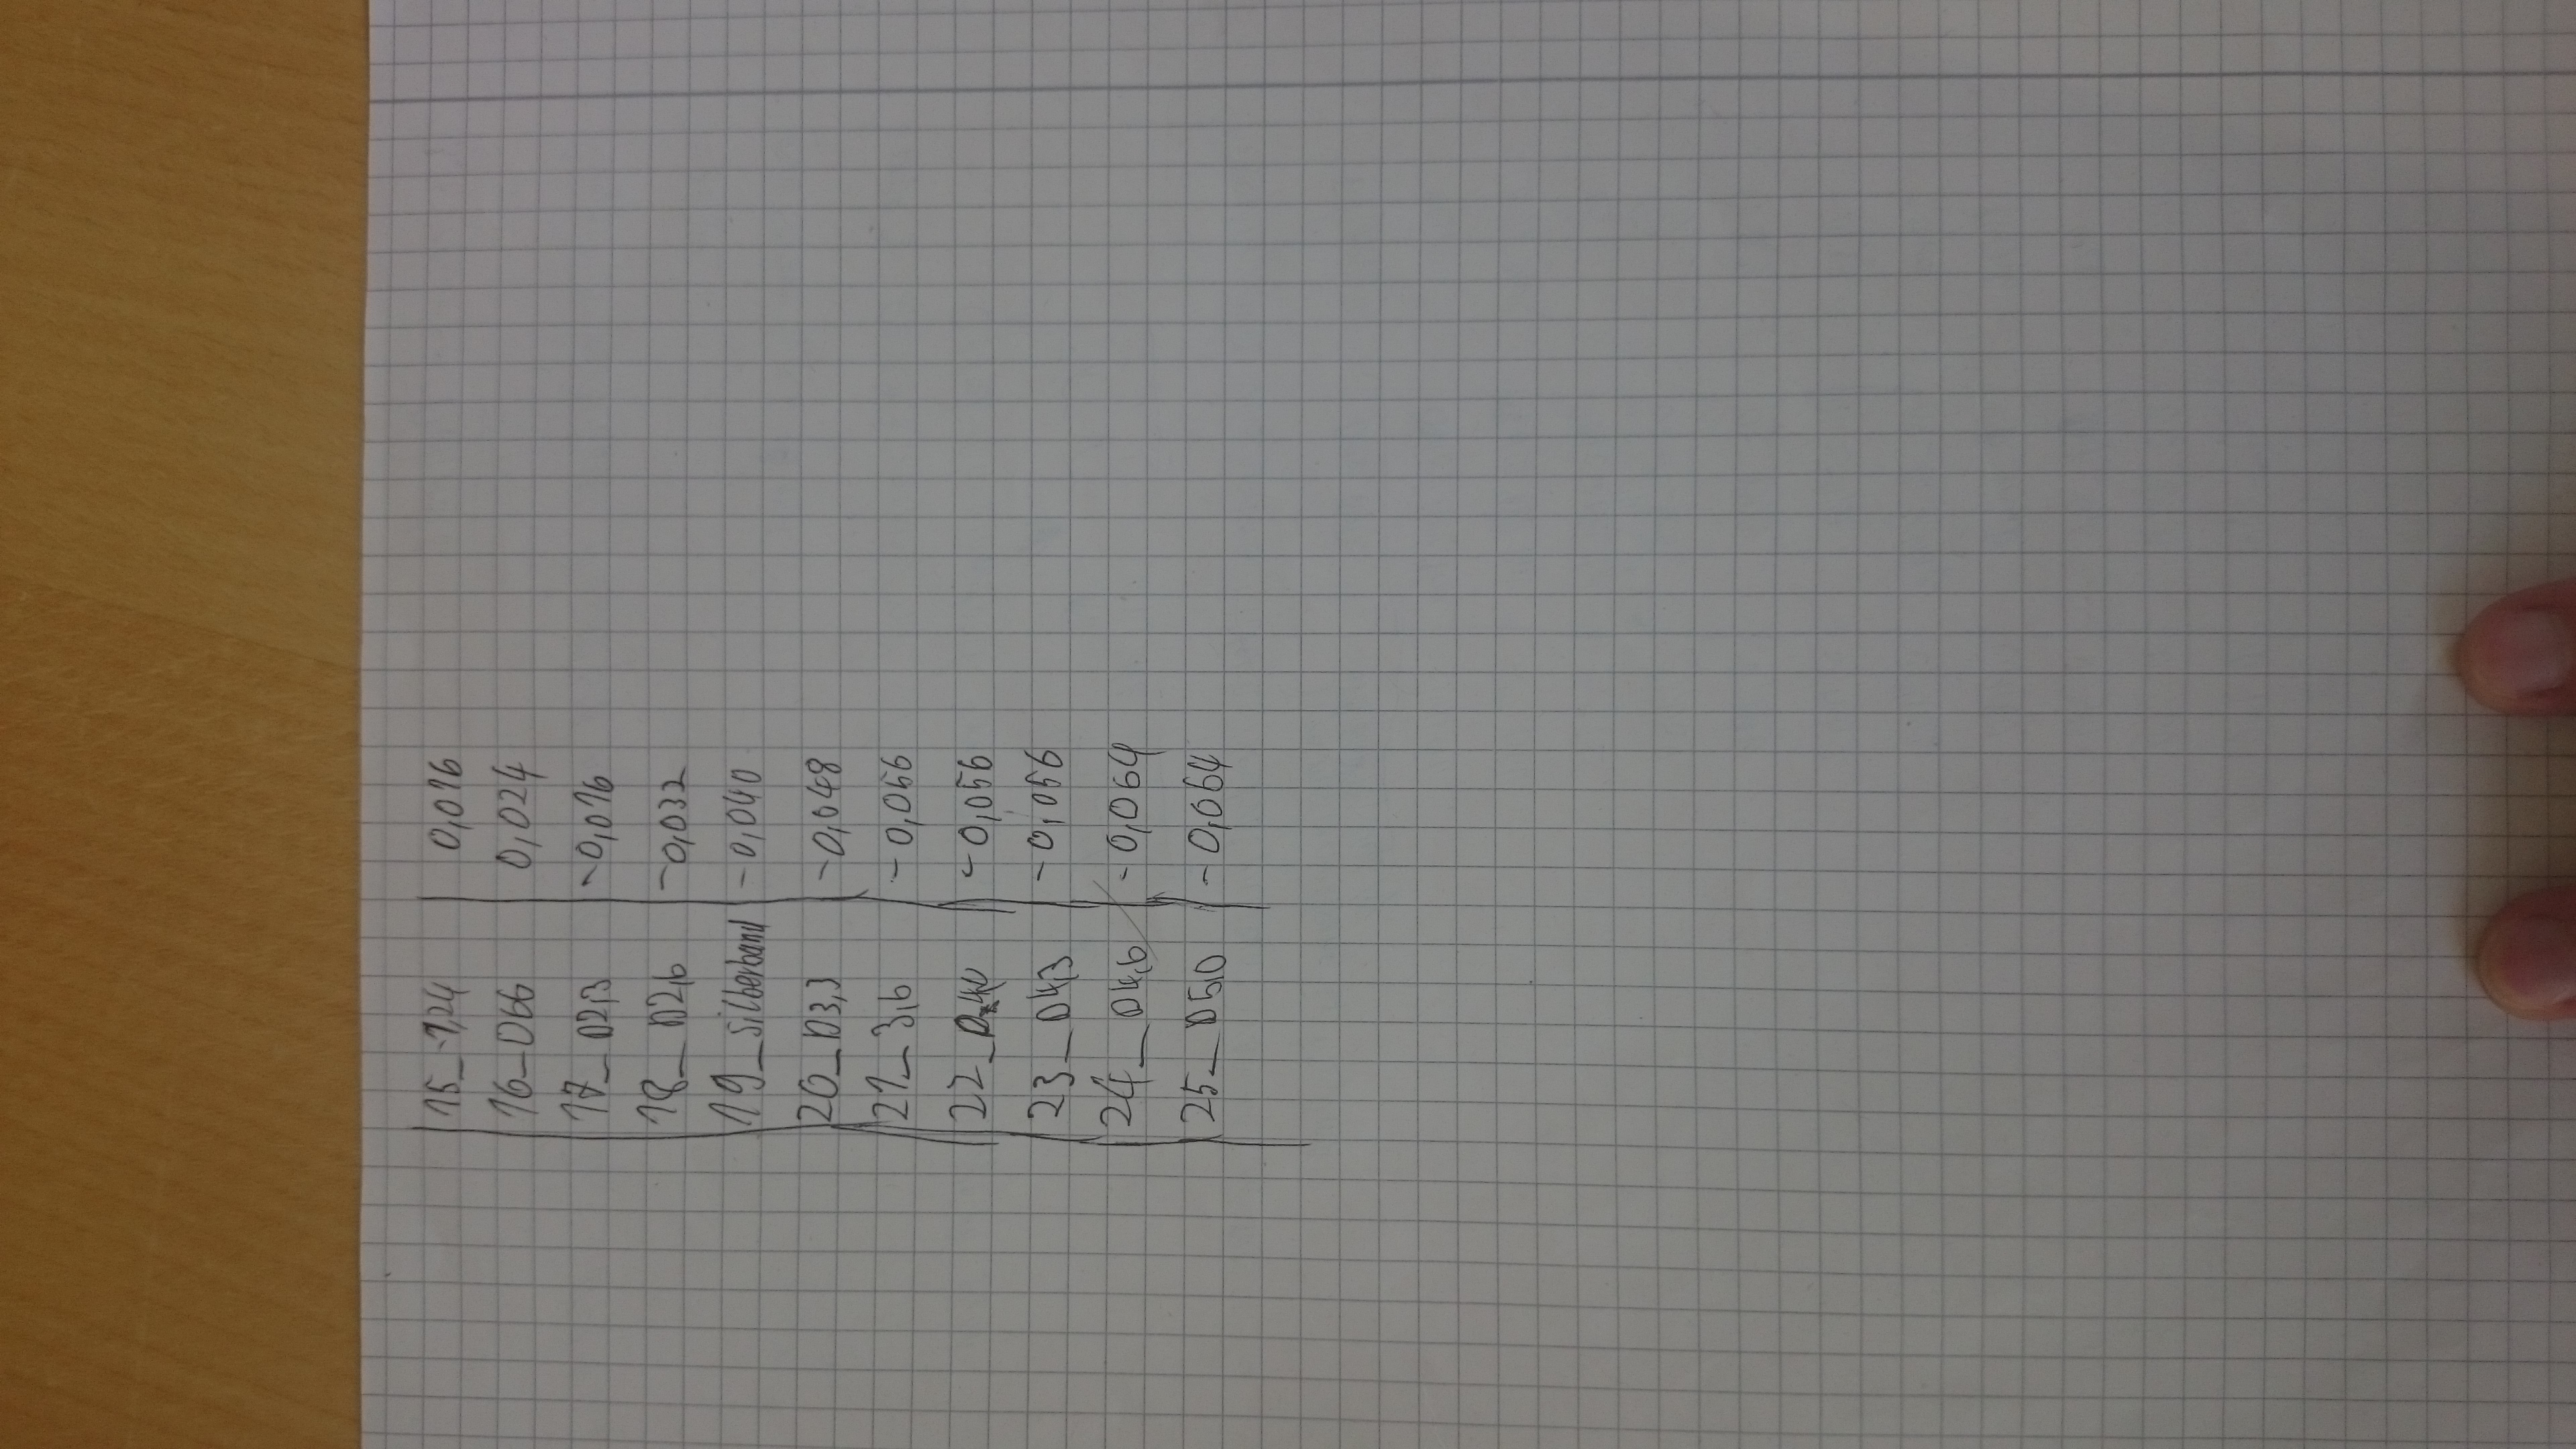
\includegraphics[angle=-90,width=1.0\linewidth]{graphics/DSC_0091}
\newpage
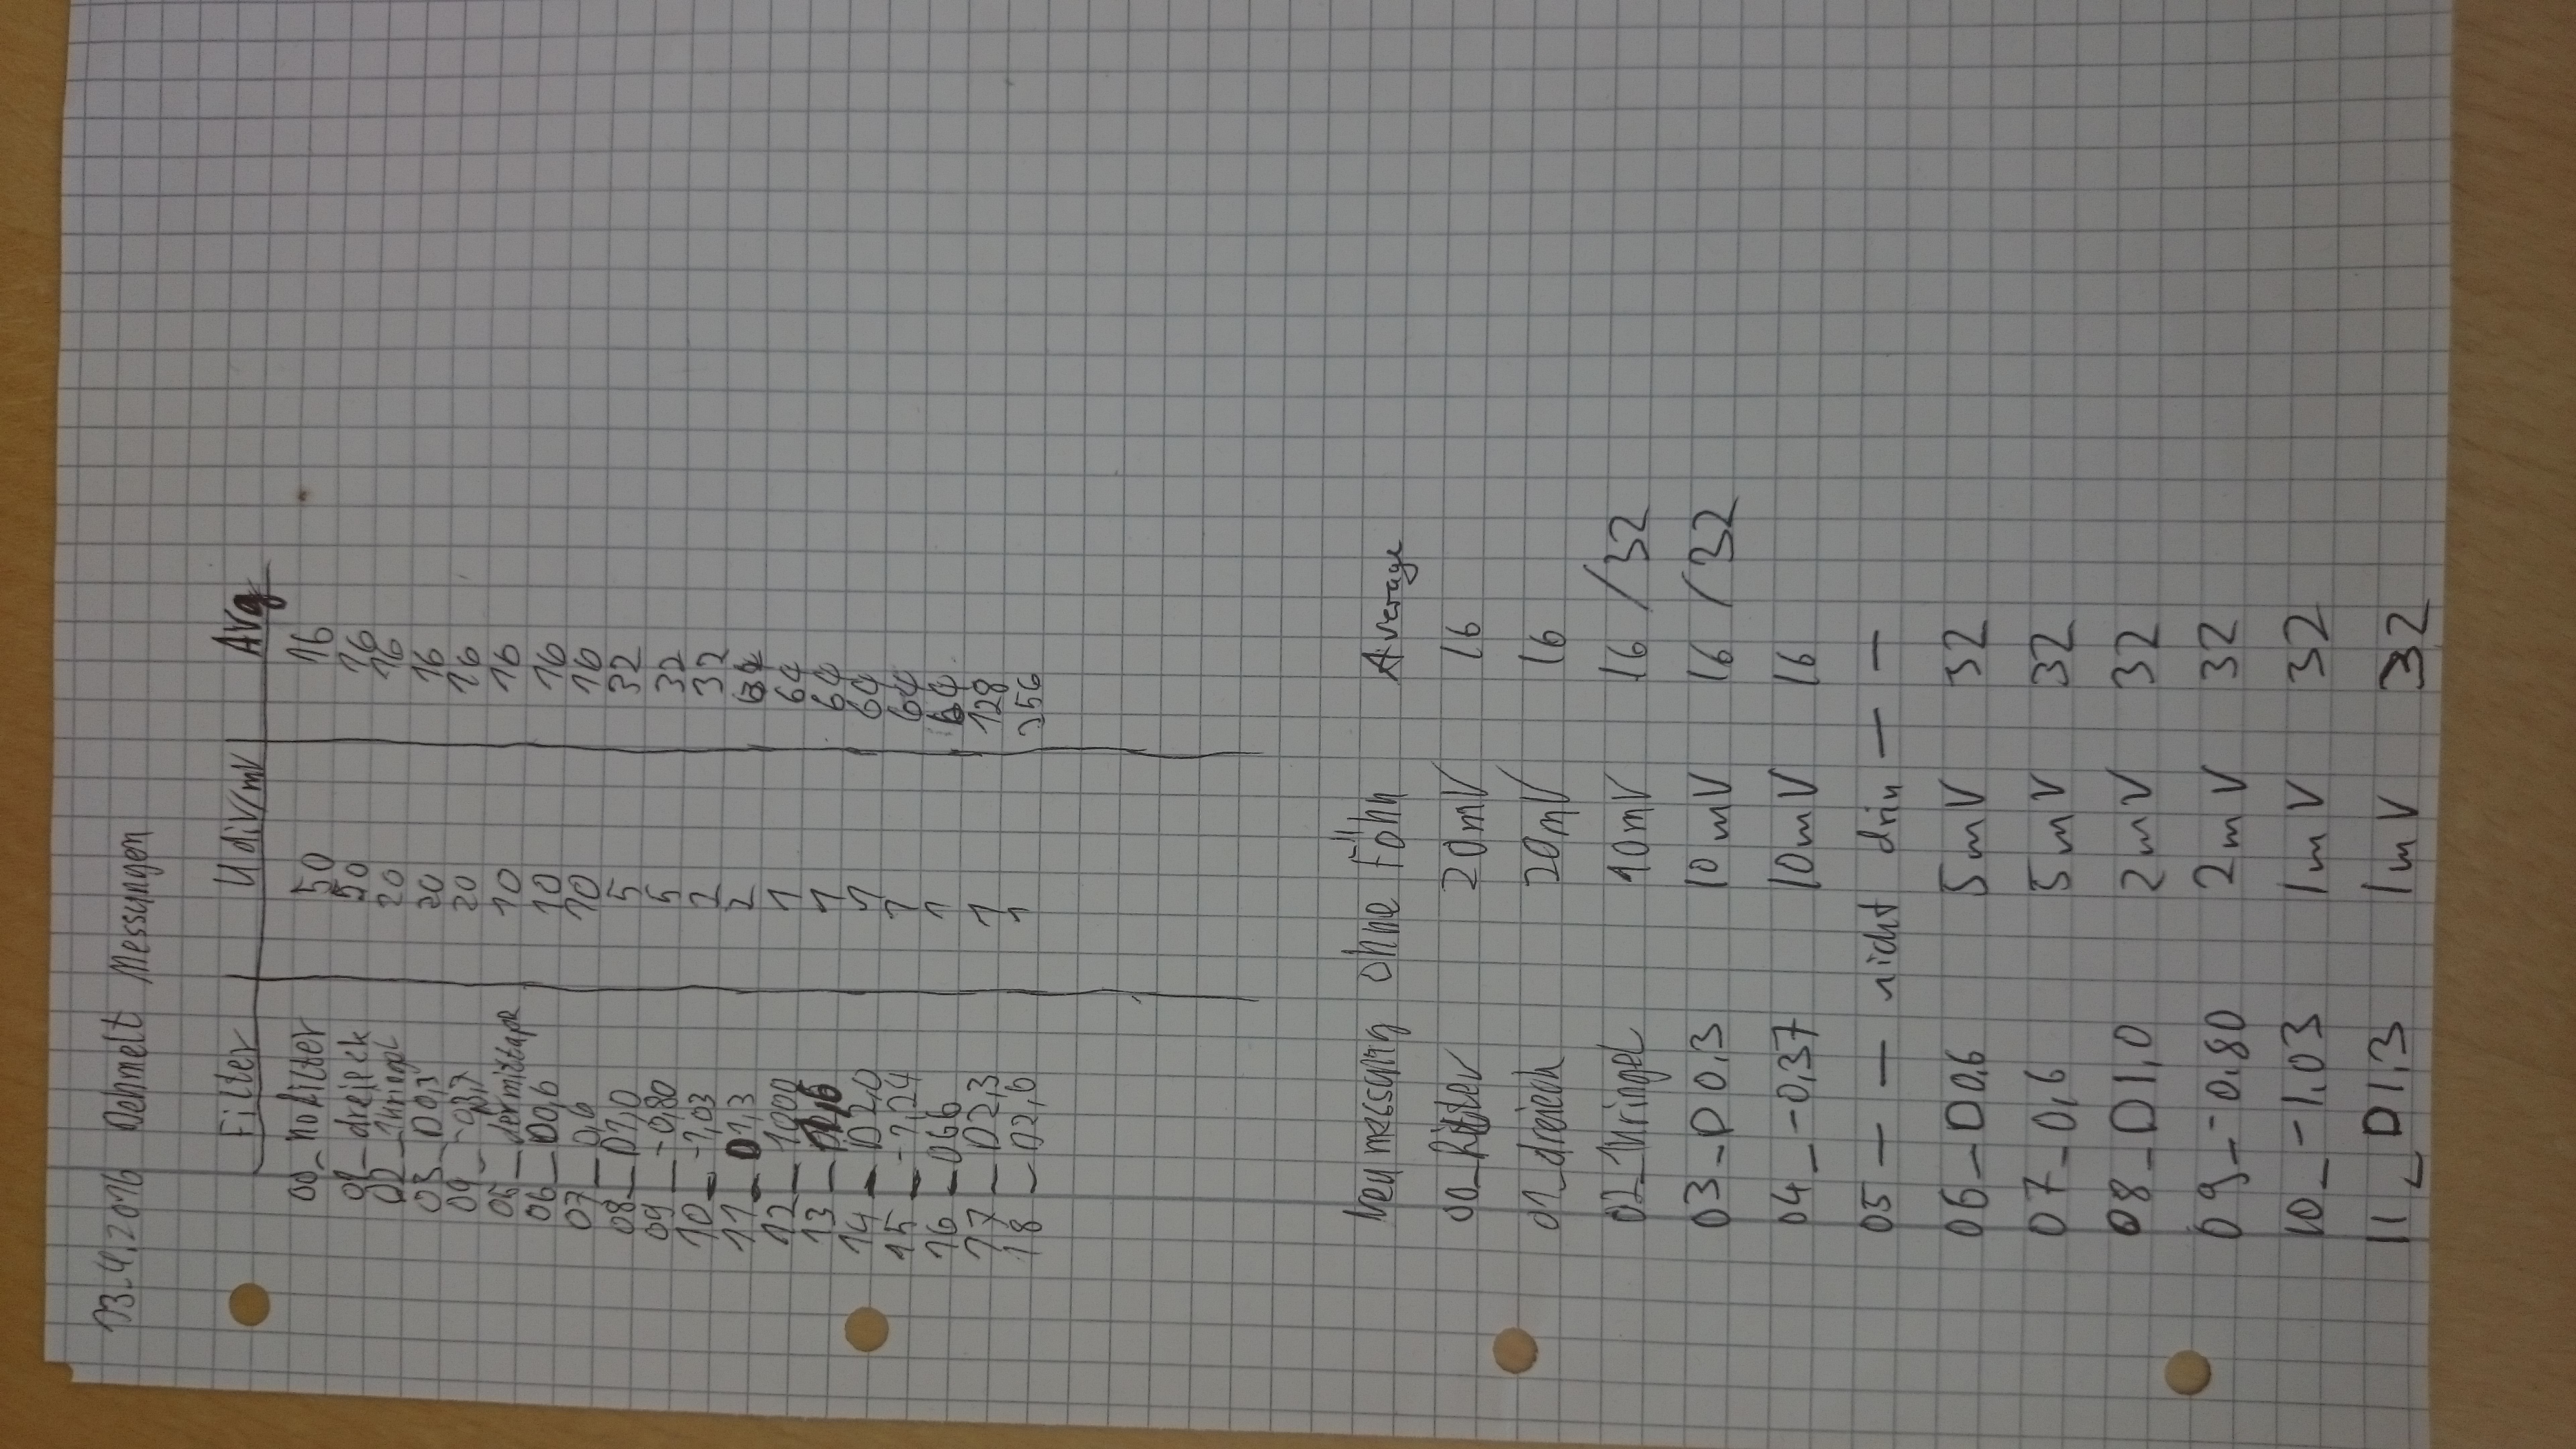
\includegraphics[angle=-90,width=1.0\linewidth]{graphics/DSC_0092}
\newpage
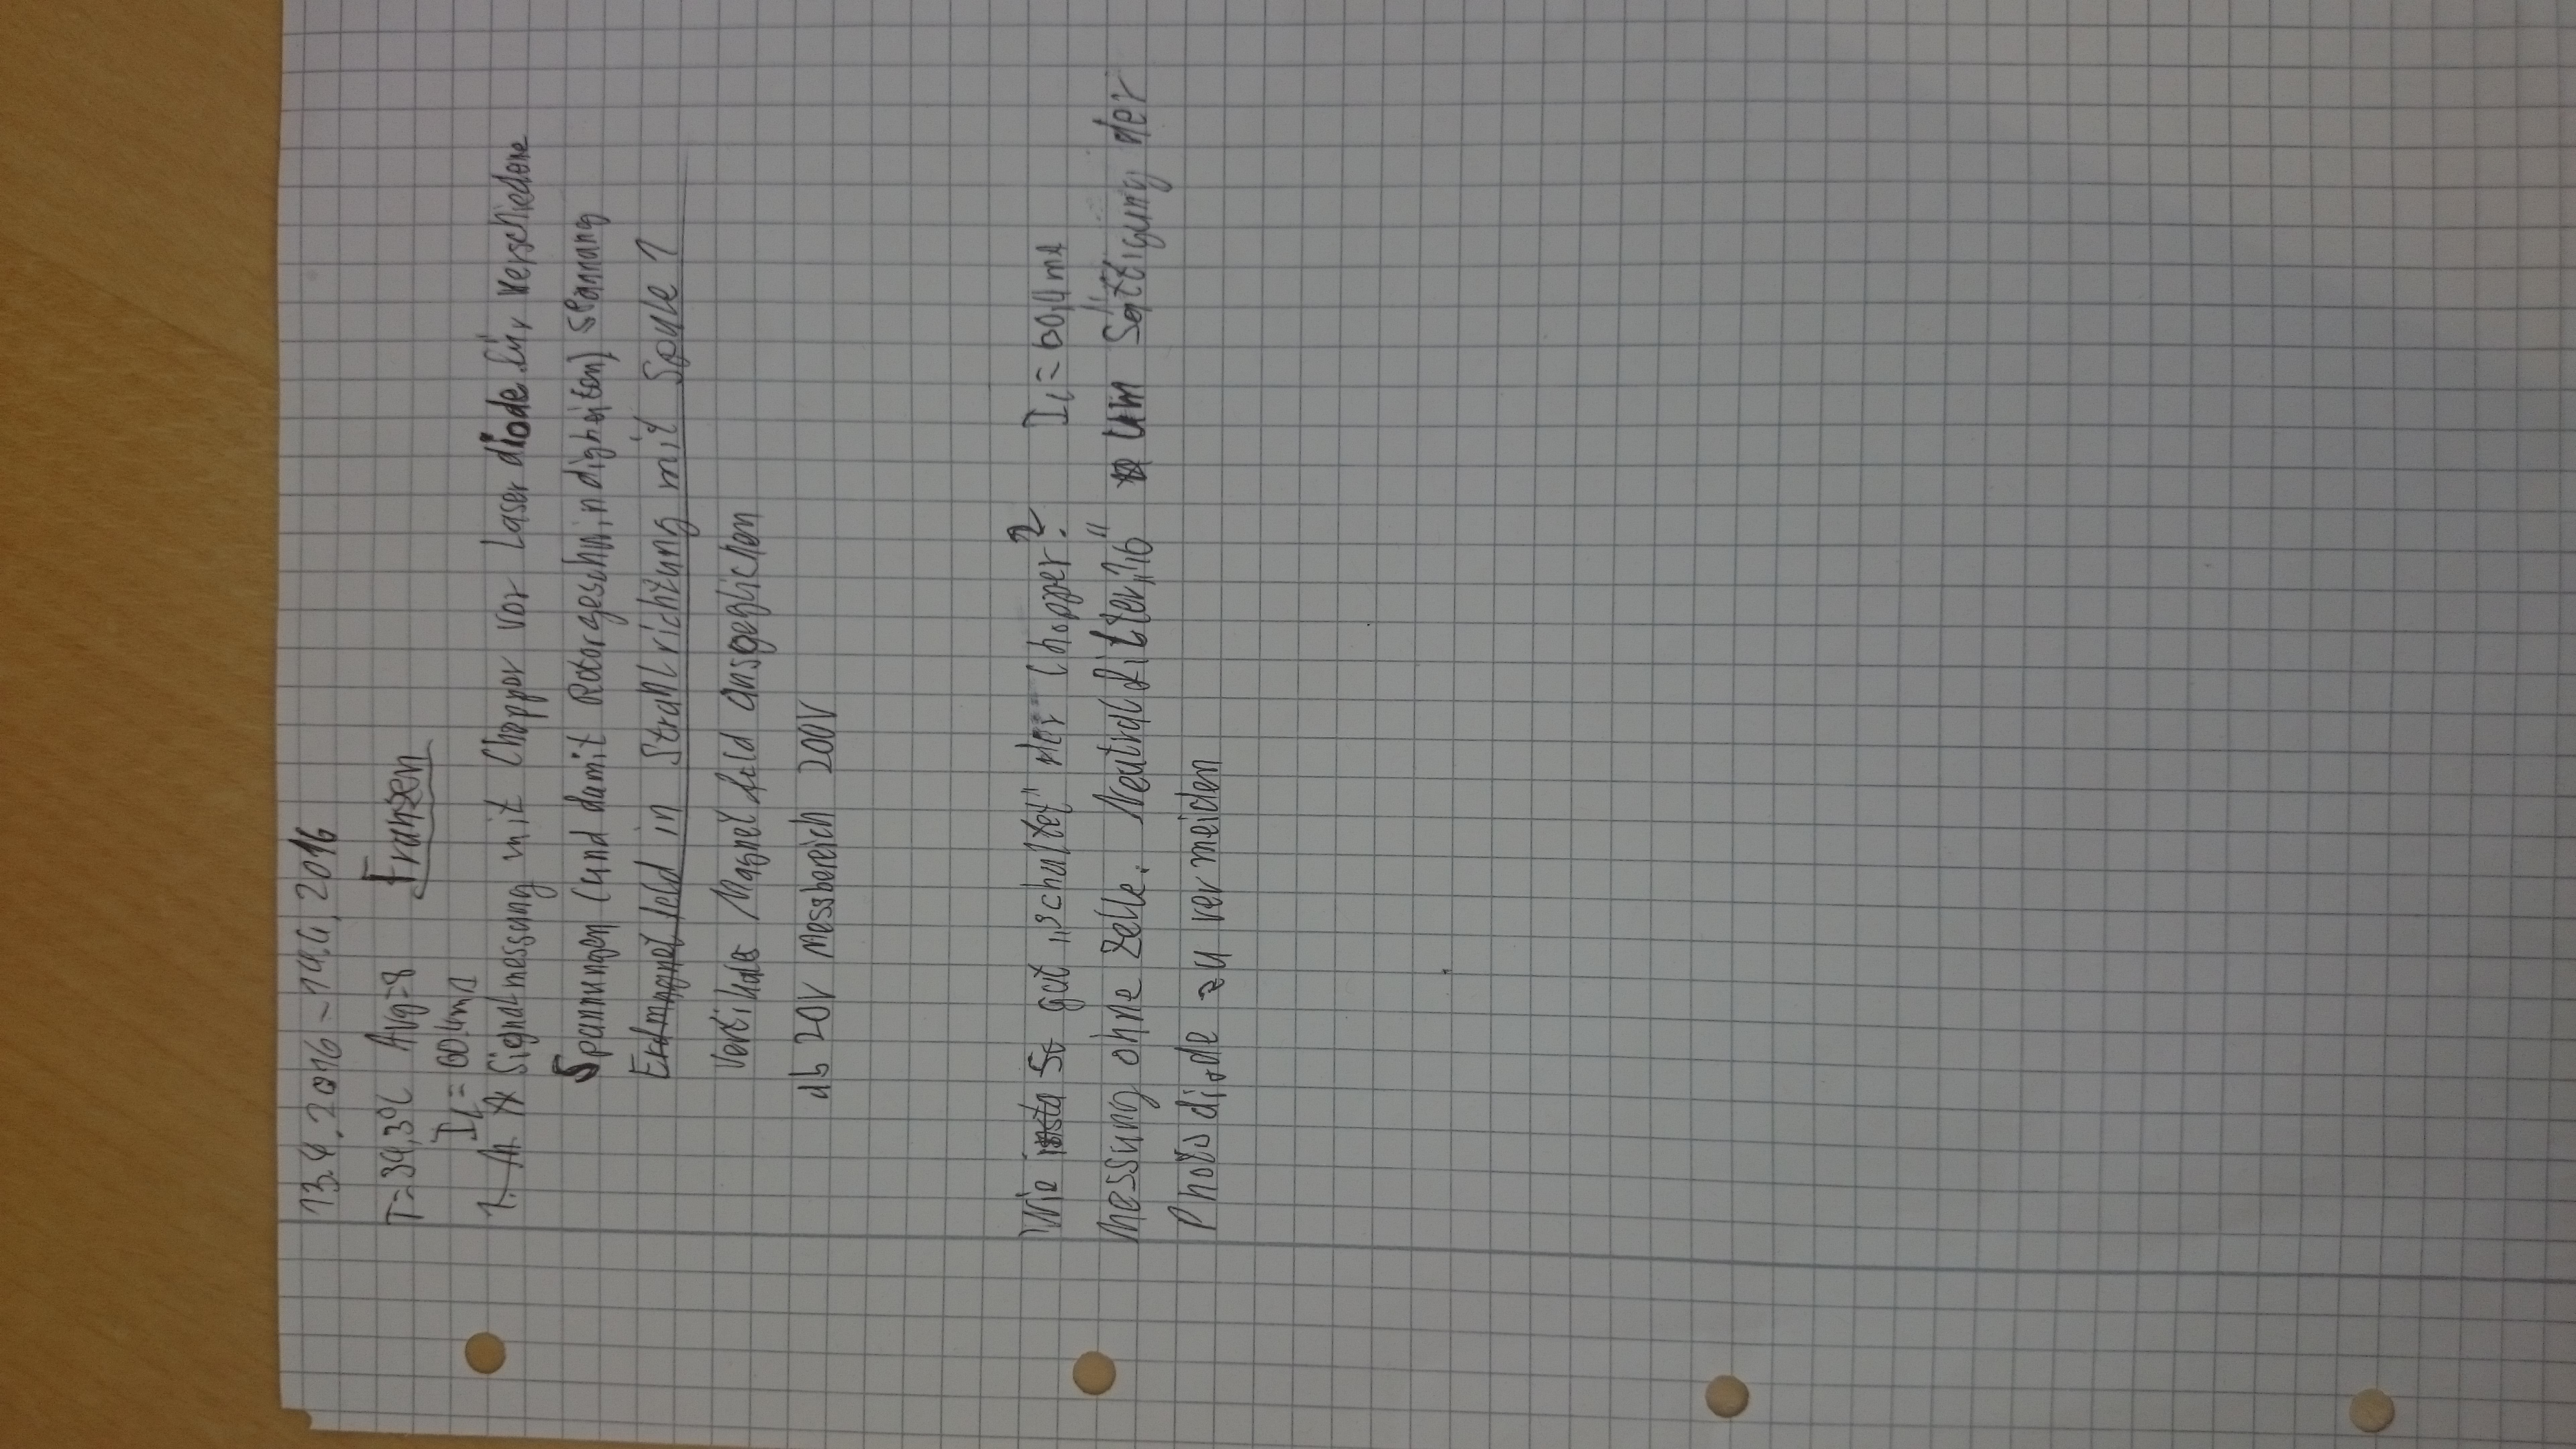
\includegraphics[angle=-90,width=1.0\linewidth]{graphics/DSC_0094}
\newpage
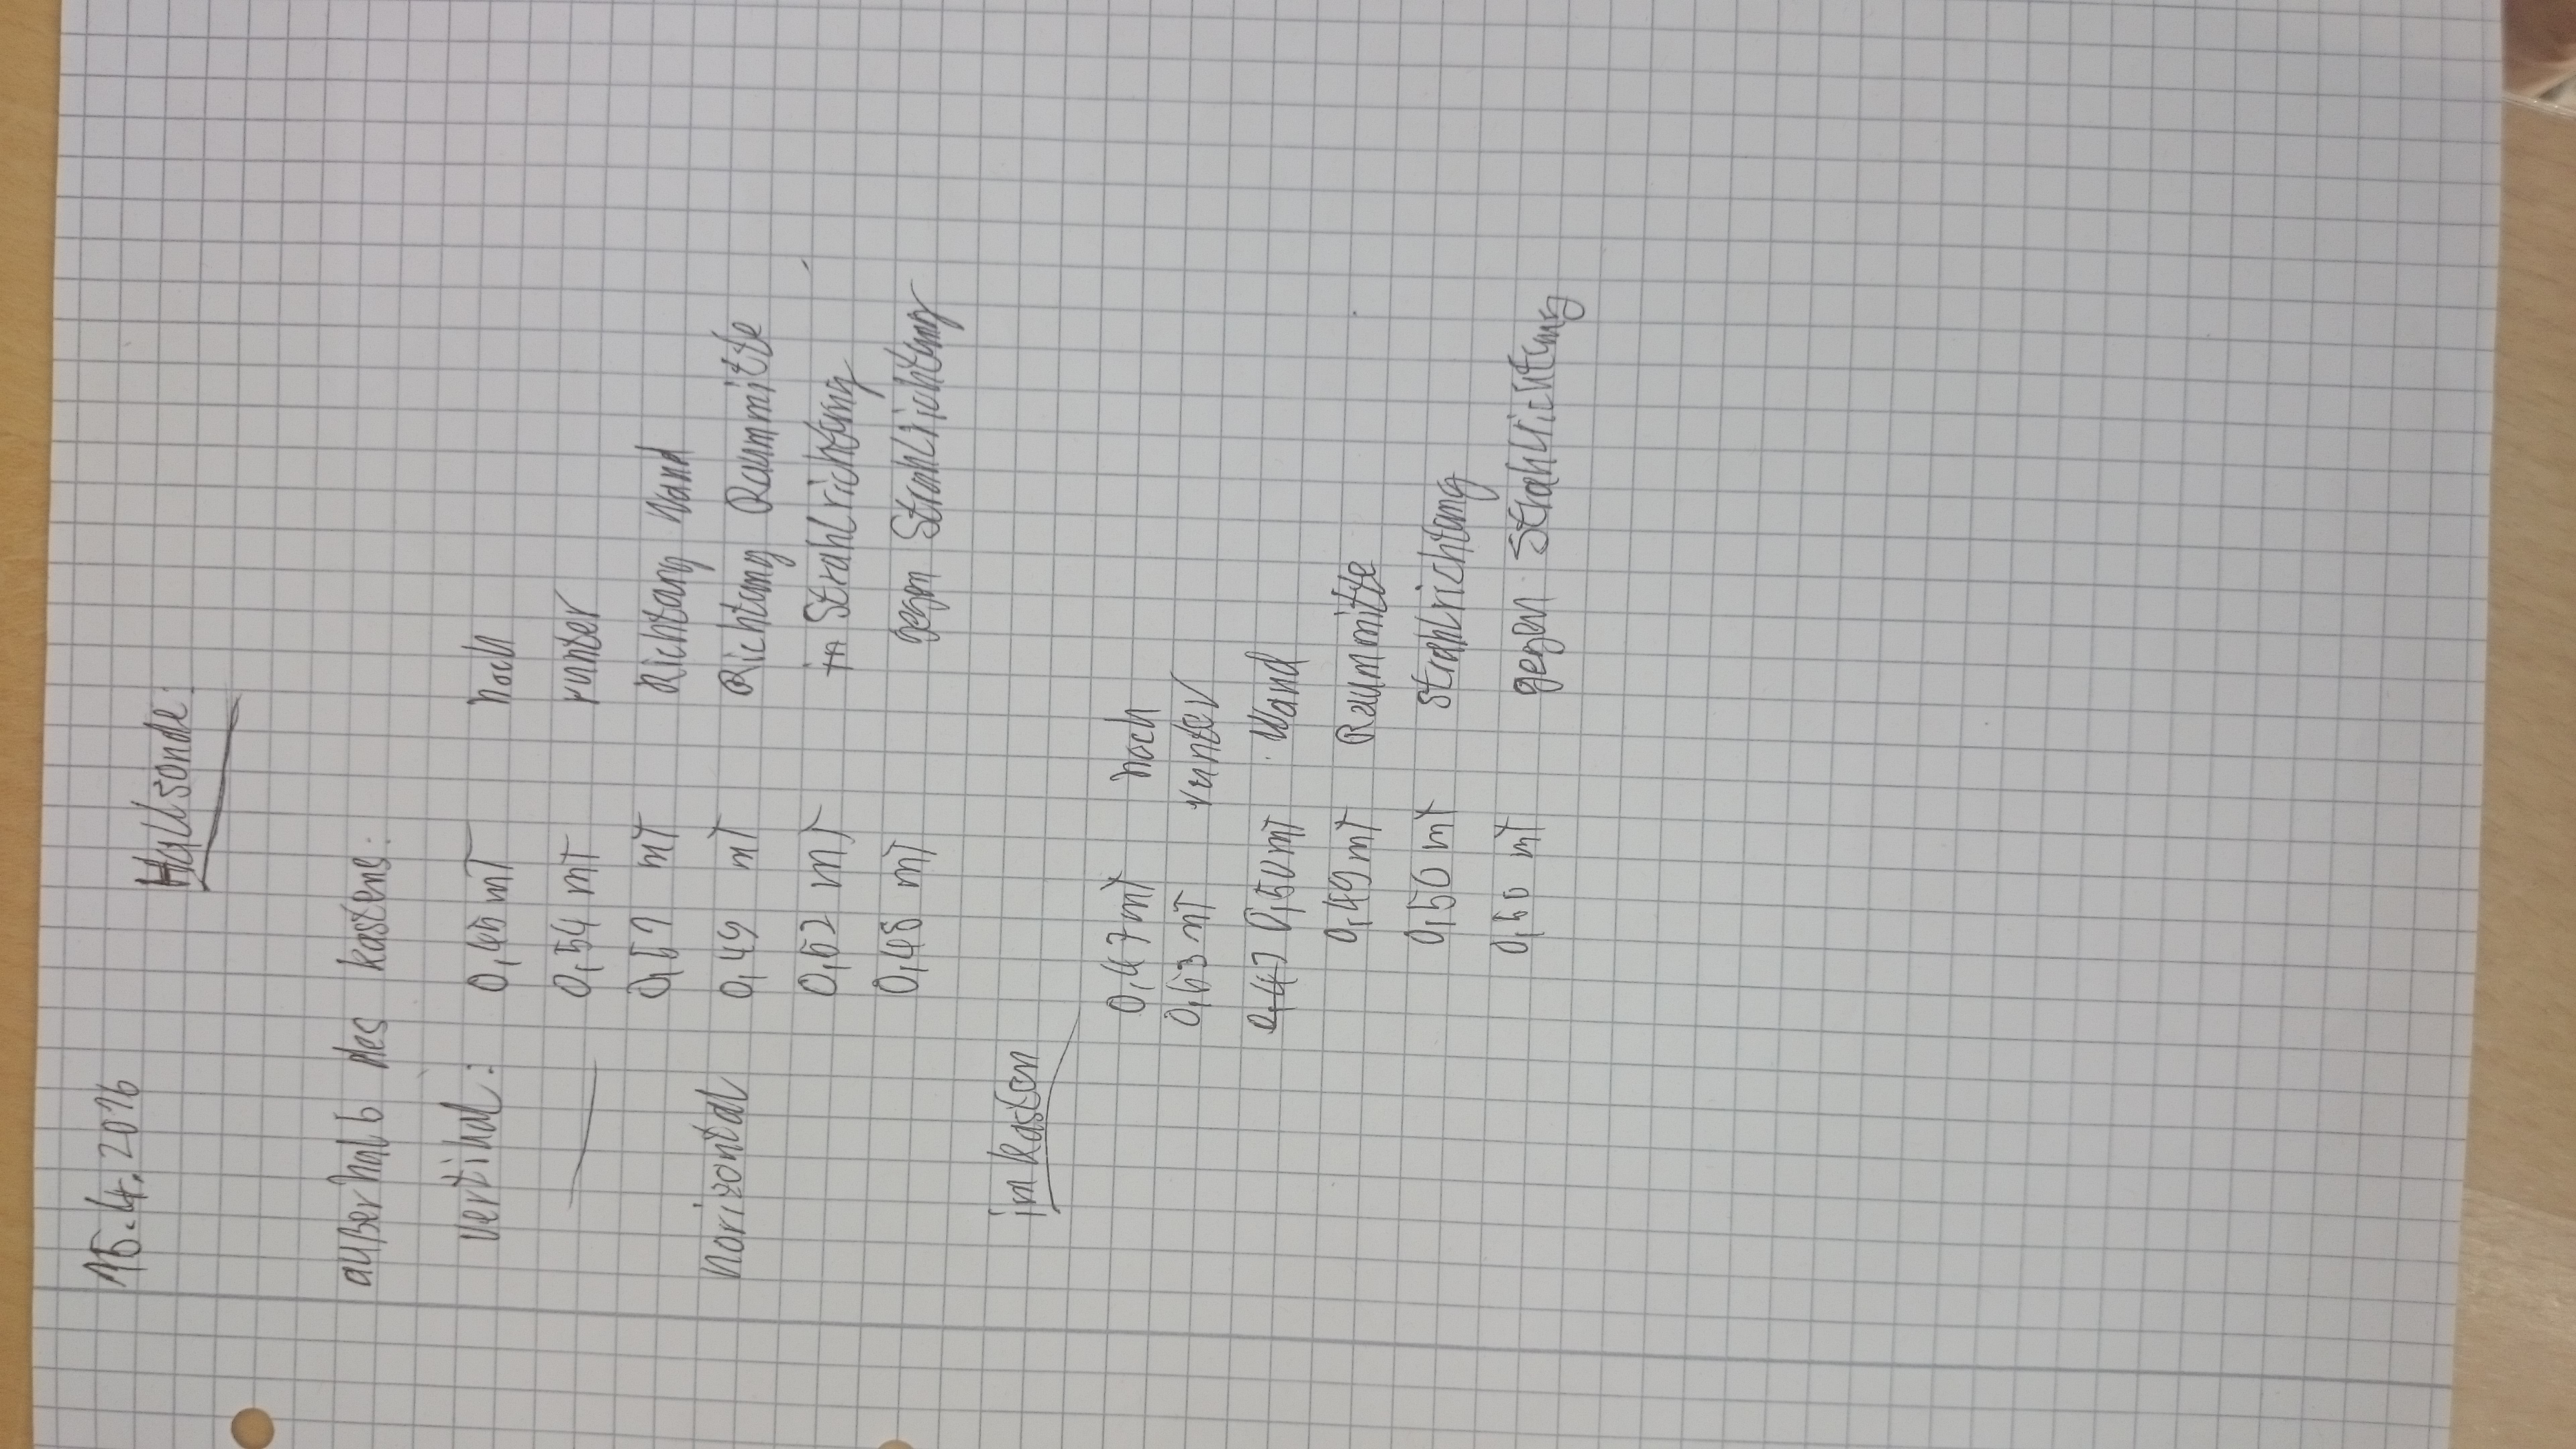
\includegraphics[angle=-90,width=1.0\linewidth]{graphics/DSC_0095}
\newpage
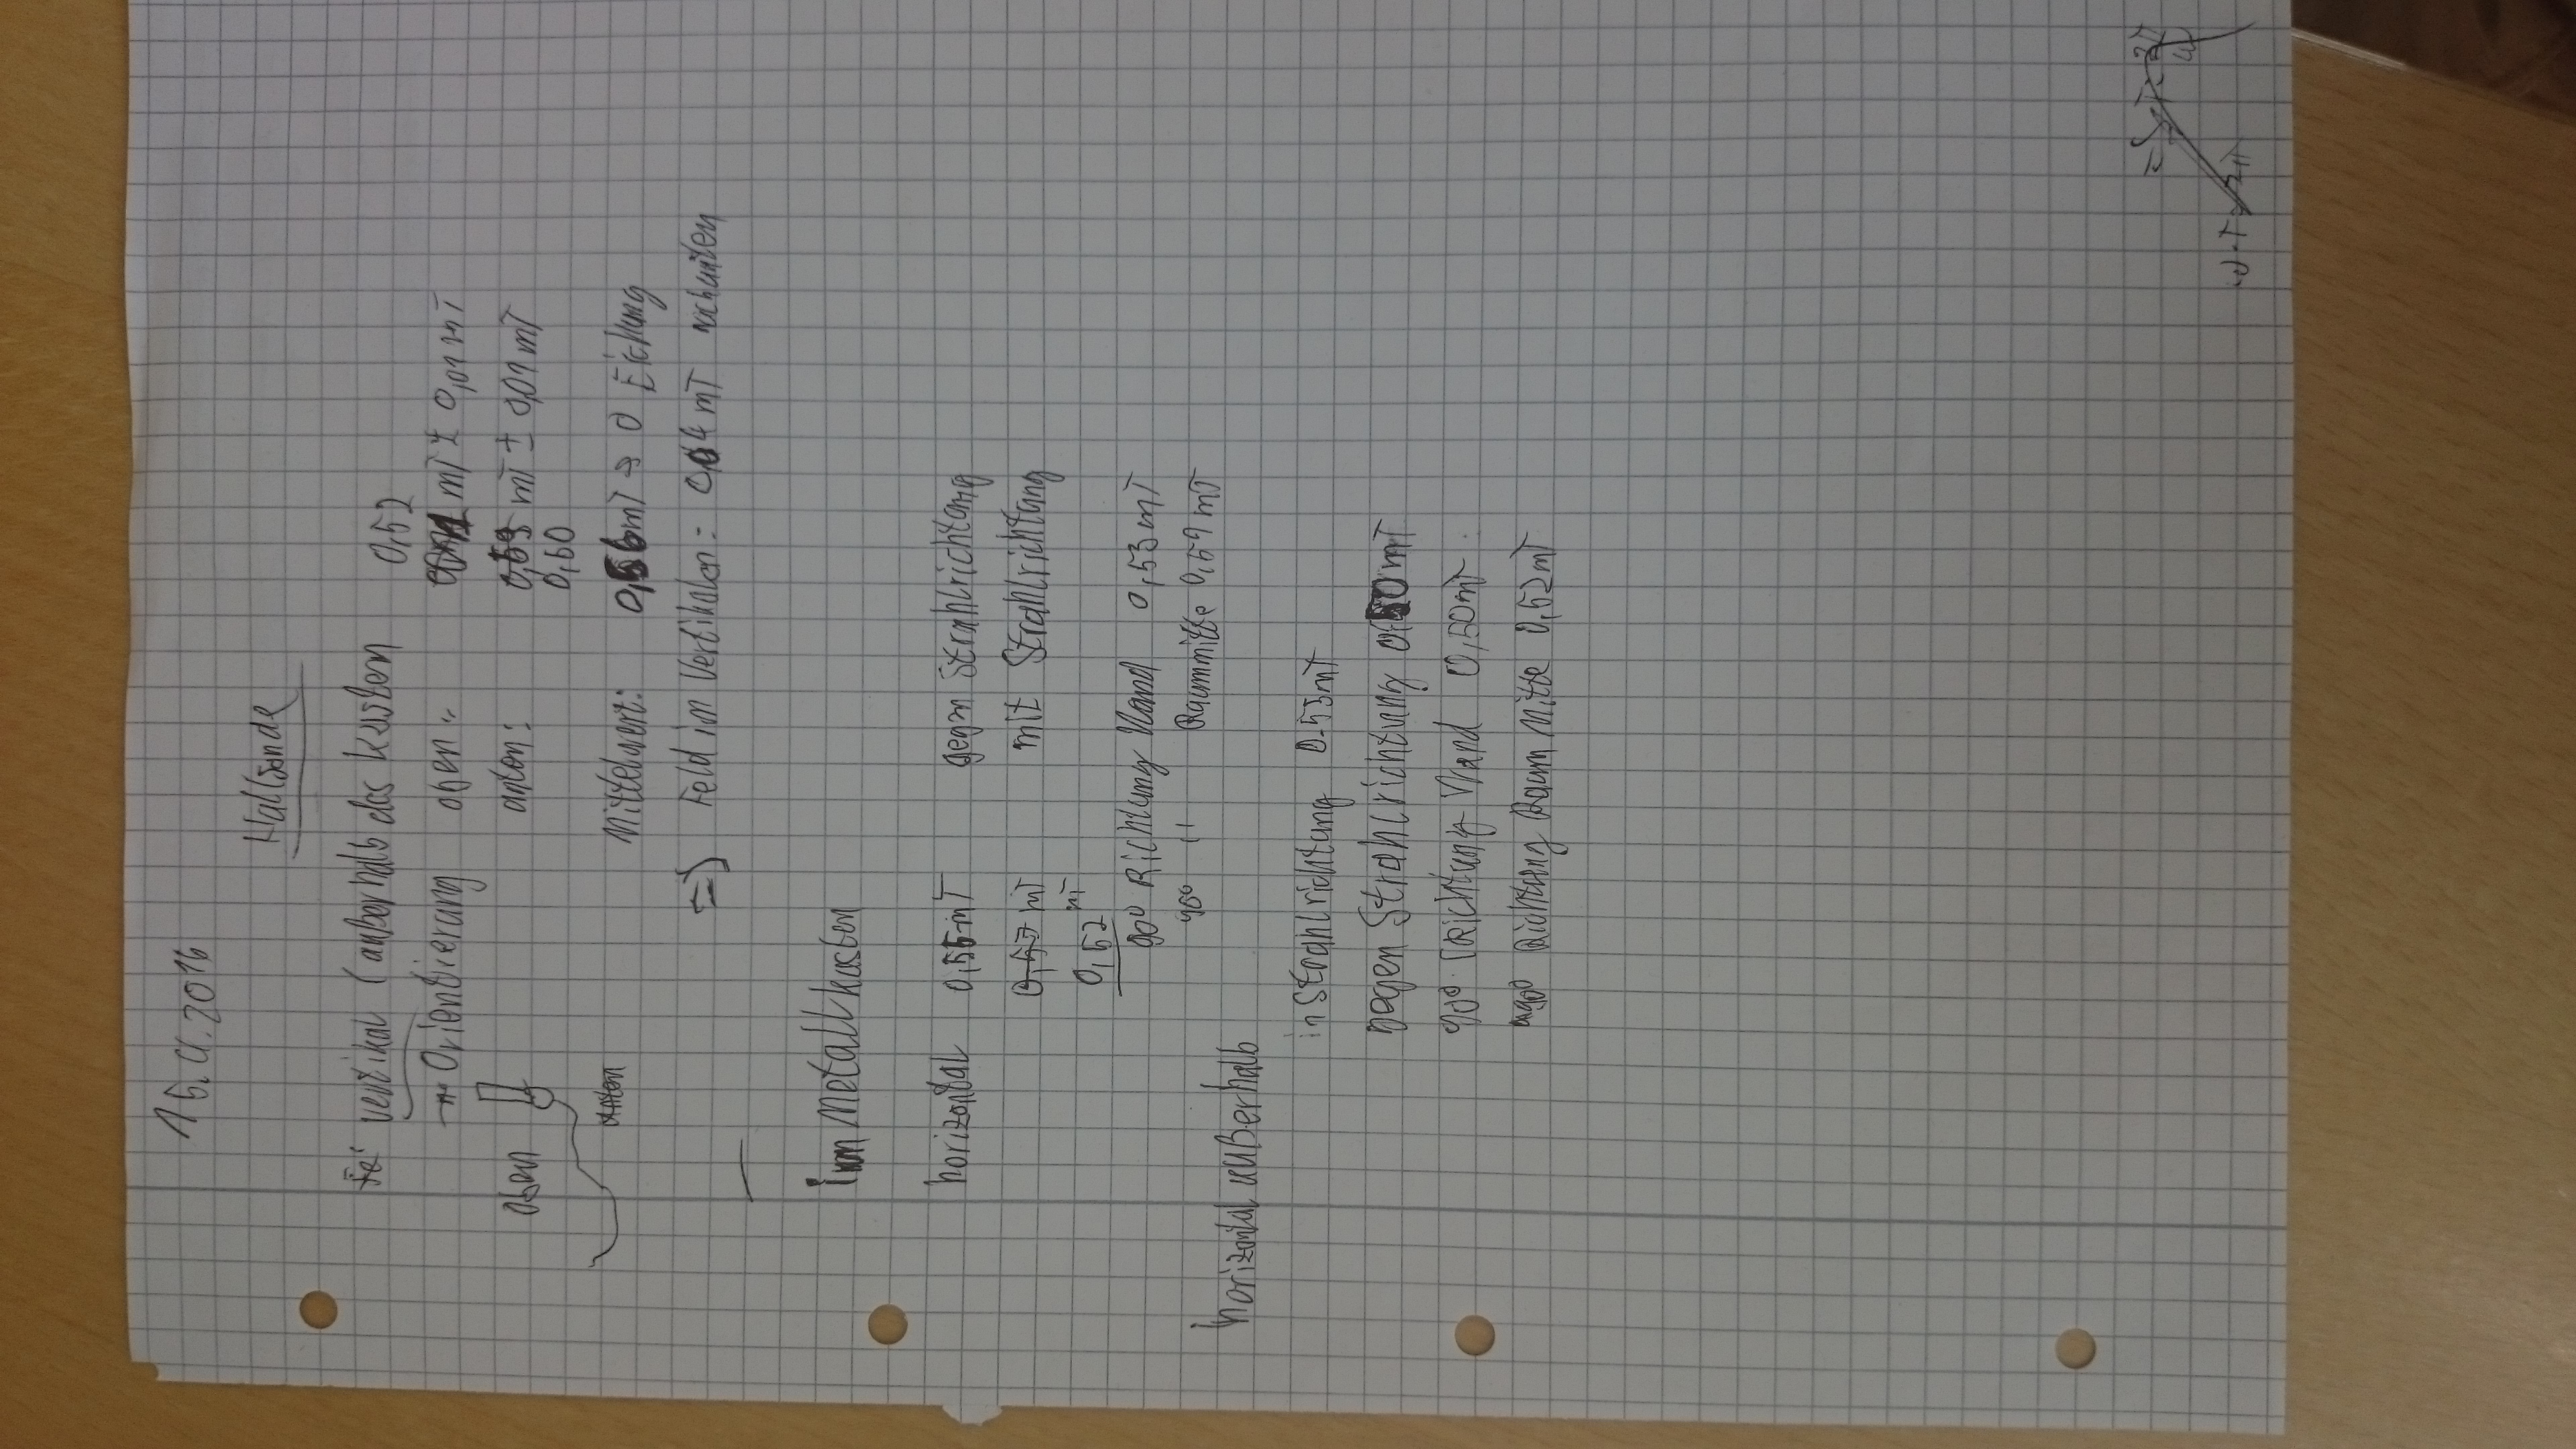
\includegraphics[angle=-90,width=1.0\linewidth]{graphics/DSC_0096}
\newpage
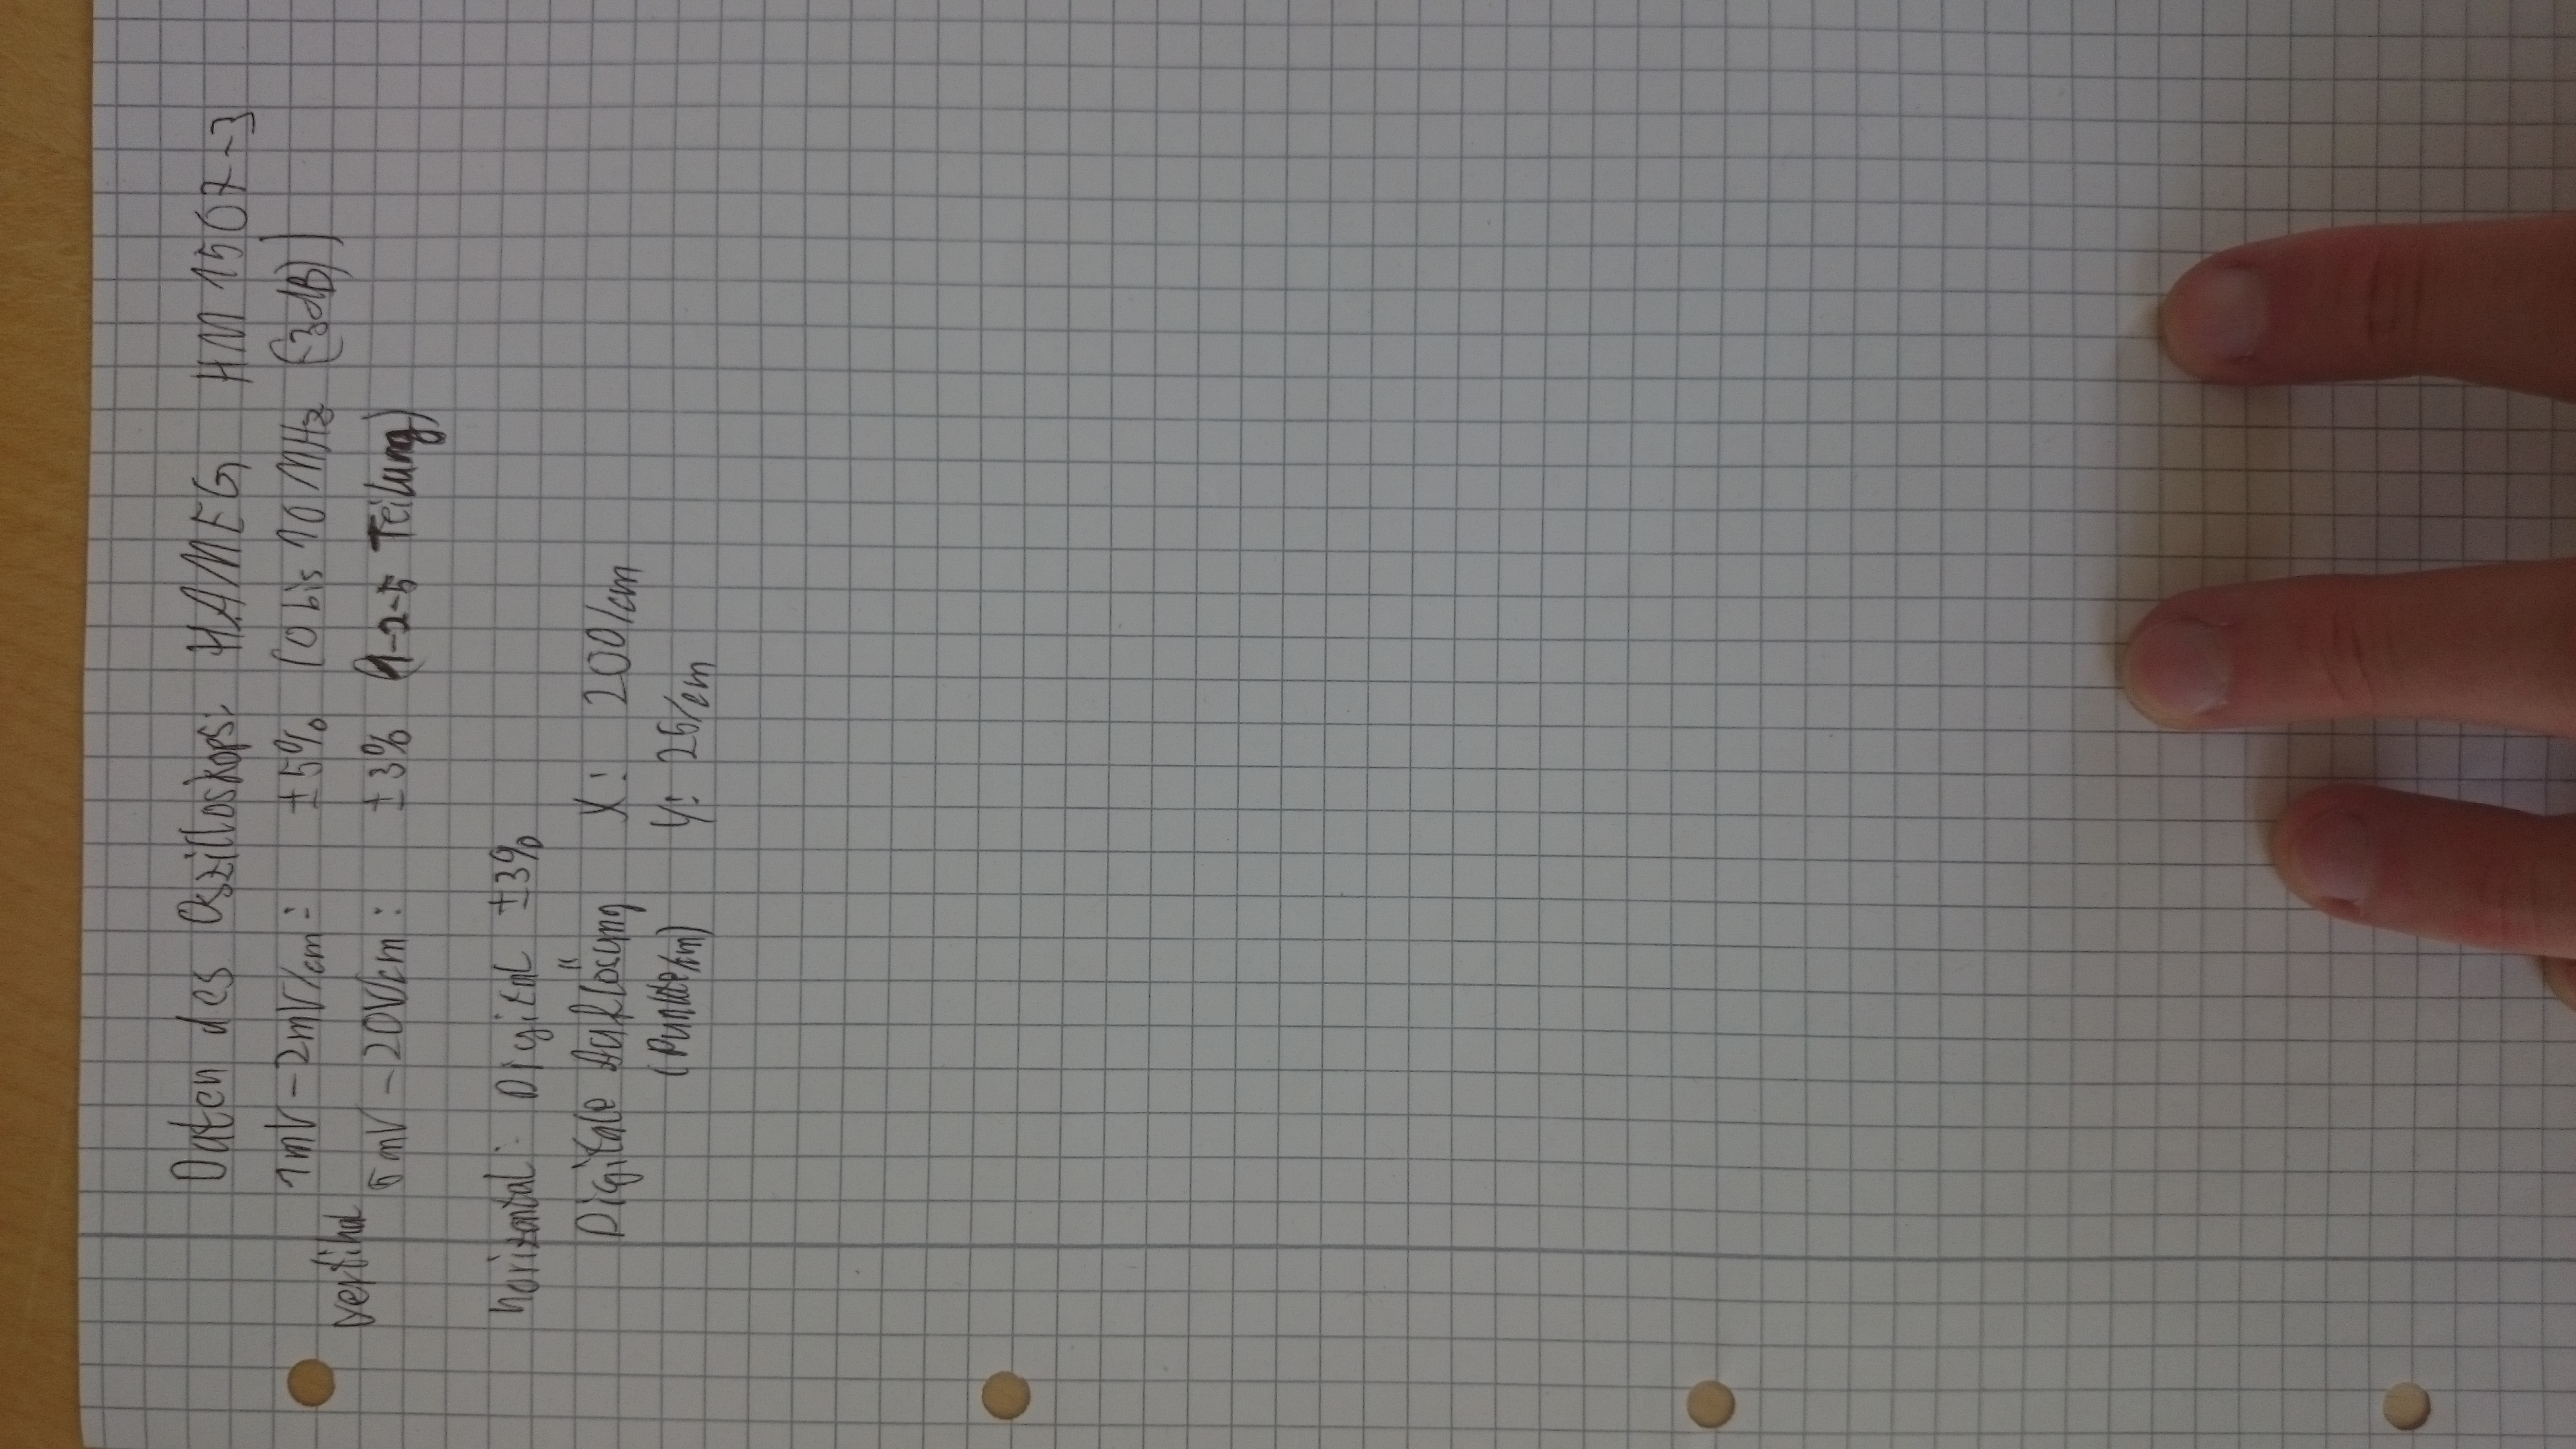
\includegraphics[angle=-90,width=1.0\linewidth]{graphics/DSC_0097}

\end{document}
